%% Los cap'itulos inician con \chapter{T'itulo}, estos aparecen numerados y
%% se incluyen en el 'indice general.
%%
%% Recuerda que aqu'i ya puedes escribir acentos como: 'a, 'e, 'i, etc.
%% La letra n con tilde es: 'n.

\chapter{Simulaciones y aplicación a una imagen real}
\label{ResultadosEmpiricos}

%\section{Estimador Propuesto}

%Se ha demostrado que esta distribución es capaz de caracterizar un gran número de objetivos en las imágenes SAR, en particular, las monopolarizadas que son las estudiadas en esta tesis. La distribución está caracterizada por tres parámetros: el número de looks $L$ que se puede estimar en toda la imagen, un parámetro de escala $\gamma$, y un parámetro de textura $\alpha$. Este último está estrechamente relacionado con el número
%de retrodispersores elementales para cada píxel, esto es una de las razones por las que recibe atención en la literatura. 
%
%Otras de las razones es que el parámetro $\alpha$ de la distribución $\mathcal{G}_I^0$ puede interpretarse en términos de la textura de la imagen. Valores cercanos a $0$, típicamente $\alpha \in [-3,0)$ sugieren zonas extremadamente texturadas como zonas urbanas. Conforme el valor de $\alpha$ decrece disminuye la heterogeneidad de la imagen. Regiones con moderada textura como son los bosques, están representadas por valores de $\alpha \in [-6,-3)$, zonas de pastura son compatibles con valores de $\alpha \in (-\infty,-6)$. Esta es otra de las razones por las cuales es muy importante obtener estimaciones precisas de este parámetro.

%Entre las técnicas de estimación disponibles, el método de los momentos y el método de Máxima Verosimilitud son las técnicas clásicas de estimación paramétrica. En \citet{Bian2013} los autores proponen un método basado en
%momentos fraccionarios de bajo orden para estimar la matriz de covarianza en una imagen SAR polarimétrica bajo una distribución alfa estable. En  \citet{VasconcellosFrerySilva:CompStat,CribariFrerySilva:CSDA} los autores utilizan técnicas de remuestreo para mejorar el rendimiento de estos estimadores en términos de sesgo y error cuadrático medio, a expensas de un alto costo computacional.

%Más recientemente \citet{MellinAnalysisPolSAR,BujorTrouveValetNicolas2004,khan2014} los estimadores basados en la transformada de Mellin, como lo son los  Logcumulantes y Logmomentos estimadores, han sido implementados con éxito. 
%Si bien Tison et al. \citet{Tison2004} mostraron que los estimadores LC tienen una mejor performance respecto del MV estimador para el modelo $\mathcal G^0$ para datos de amplitud, estos estimadores no han sido evaluados para el caso de datos de intensidad ni bajo la presencia de contaminación.

%Una propiedad que es deseable que un estimador posea es ser resistente a la presencia de datos atípicos. Bustos et al. \citet{BustosFreryLucini:Mestimators:2001} y Allende et al. \citet{AllendeFreryetal:JSCS:05} estudiaron la performance del MV estimador bajo el modelo $\mathcal{G}^{0}$ para datos de amplitud, mostrando que hay una pérdida de robustez ante la presencia de outliers moderados en áreas extremadamente texturadas, mientras que para zonas texturadas la pérdida de robustez ocurre en presencia de outliers severos. Asimismo esta falta de robustez es más pronunciada en el caso de muestras de pequeño tamaño. Ellos propusieron como alternativa los M y AM estimadores que tienen un buen comportamiento bajo contaminación pero presentan problemas numéricos especialmente para tamaños de muestras chicos.

El aporte principal de esta tesis es presentar un nuevo método de estimación para el parámetro de textura del modelo $\mathcal{G}_I^0(\alpha,\gamma,L)$ que tenga  buenas propiedades midiéndolas en término de su sesgo, su error cuadrático medio, su capacidad para resistir diferentes niveles de contaminación, de bajo costo computacional y que tenga un buen comportamiento incluso para muestras de tamaño pequeño y moderado. 

Para ello porponemos como estimador del parámetro de textura al valor del argumento que minimiza la distancia estocástica entre el modelo teórico y una estimación no paramétrica de la función de densidad subyacente, es decir,
\begin{align}
\label{PropuestaMDE}
\widehat{\alpha}=\mathop{\rm argmin} \limits_{\alpha} d(f_{\alpha}, \widehat{f}_n)
\end{align}
donde $d$ es una medida de discrepancia, discimilaridad o distancia estocástica, entre la función de densidad teórica $f_{\alpha}$ y un estimador no paramétrico $\widehat{f}_n$ de dicha función de densidad.

Esta propuesta está basada en dos pilares: la forma de estimar $\widehat{f}_n$ y la distancia estocástica elegida. En este capítulo daremos argumentos que sugieren que los núcleos asimétricos ofrecen una buena alternativa para estimar la función de densidad subyacente en forma no paramétrica, en particular los núcleos $\Gamma$ y LN son una buena elección. También proponemos el método para elegir el ancho de banda, como así también mostraremos que la distancia triangular es una buena medida de discrepancia para este caso.

Se comparará el comportamiento del estimador $\widehat{\alpha}$ con los estimadores MOM, MV y LC definidos en las subsecciones~\ref{MetodoMOM},~\ref{MetodoMV} y~\ref{MetodoLC} respectivamente a través de un estudio de simulación Monte Carlo, como así también mediante la aplicación a una imagen real.

\section{Generando muestras $\mathcal{G}_I^0$}

Para generar muestras que provengan de una distribución $\mathcal{G}_I^0$ vamos a explotar la naturaleza multiplicativa del modelo que la genera.

De acuerdo a la sección~\ref{ModeloGI0} la distribución  $\mathcal{G}_I^0$ es el producto de las distribuciones $\Gamma^{-1}(-\alpha,\gamma)$ y $\Gamma(L,L)$ donde $-\alpha, \, \gamma >0$ y $L\geq 1$. Además, se sabe que si $X \sim \Gamma(a,\beta)$, entonces $Y = 1/X \sim \Gamma^{-1}(a,\beta)$.

Luego, para generar una muestra $Z_1, \ldots, Z_n$ de variables aleatorias independientes e idénticamente distribuidas con $Z_i \sim \mathcal{G}_I^0(\alpha,\gamma,L)$ con $i=1, \ldots, n$ hacemos lo siguiente:
\begin{itemize}
	\item Fijamos $a=-\alpha, \, \gamma$ ambos positivos y $L \geq 1$.
	\item Generamos una muestra de tamaño $n$ de una variable aleatoria $W \sim \Gamma(a,\gamma)$.
	\item Definimos $X=1/W$, entonces $X \sim \Gamma^{-1}(a,\beta)$.
	\item Generamos una muestra de tamaño $n$ de una variable aleatoria $Y \sim \Gamma(L,L)$.
	\item Obtenemos $Z \sim \mathcal{G}_I^0(\alpha,\gamma,L)$ definiendo $Z=X \cdot Y$.
\end{itemize}


\section{Eligiendo distancias estocásticas}
\label{EligiendoDistancias}

El primer objetivo de este trabajo fue elegir una distancia entre las posibles medidas de discimilaridad que ofrece la literatura. Como se mencionó en el capítulo~\ref{metodologia}, se consideraron las siguientes distancias estocásticas entre las densidades $f$ y $g$ de soporte común $S$:

\begin{itemize}
	\label{dist}
	\item Distancia de Hellinger $d_\text{\tiny H}(f,g)=1-\displaystyle{\int_{S}\sqrt{f g}}$.
	
	%\item Distancia de Bhattacharyya $d_\text{\tiny B}(f_\text{\tiny V},f_\text{\tiny W})=-\log\displaystyle{\int_{-\infty}^{\infty}\sqrt{f_\text{\tiny V} f_\text{\tiny W}}}$.
	
	\item Distancia Triangular $d_\text{\tiny T}(f,g)=\displaystyle{\int_{S}\frac{(f-g)^2}{f+g}}$.
	
	\item Distancia de R\'enyi con parámetro $\beta\in(0,1)$
	$$
	d_\text{\tiny R}^{\beta}(f,g)=\frac{1}{2(\beta-1)}\left[\log\displaystyle{\int_{S}\big({f^{\beta}g^{1-\beta})}+\log\displaystyle{\int_{S}\big(f^{1-\beta}g^{\beta}}}\big)\right].
	$$
\end{itemize}

Para cumplir con el objetivo inicialmente planteado comenzamos calculando las curvas de distancias entre las funciones de densidad de la distribución $\mathcal G_I^0(\alpha_0, -\alpha_0-1, L)$ y $\mathcal G_I^0(\alpha,-\alpha-1,L)$, $\alpha<-1$, para distintos valores de $\alpha_0$ y de $L$. Recordemos que vamos a considerar que el parámtetro de escala cumpla la condición $\gamma^*=-\alpha-1$ para que la $E(Z)=1$ donde $Z \sim \mathcal{G}_I^0(\alpha,\gamma,L)$. Esta relación nos brinda la posibilidad de llevar un problema de estimación de dos parámetros a estimar un sólo parámetro. 

Las figuras~\ref{DistL1},~\ref{DistL3} y~\ref{DistL8} muestran los gráficos de dichas curvas, para los casos donde el número de looks $L=1,3,8$, el valor de $\alpha_0= -2,-3,-4,-5,-6,-7$ y las distancias de Hellinger, Rényi (con parámetro $\beta=0.8$) y Triangular. 

\begin{figure}[h!]
	\centering    
	\subfigure[Hellinger]{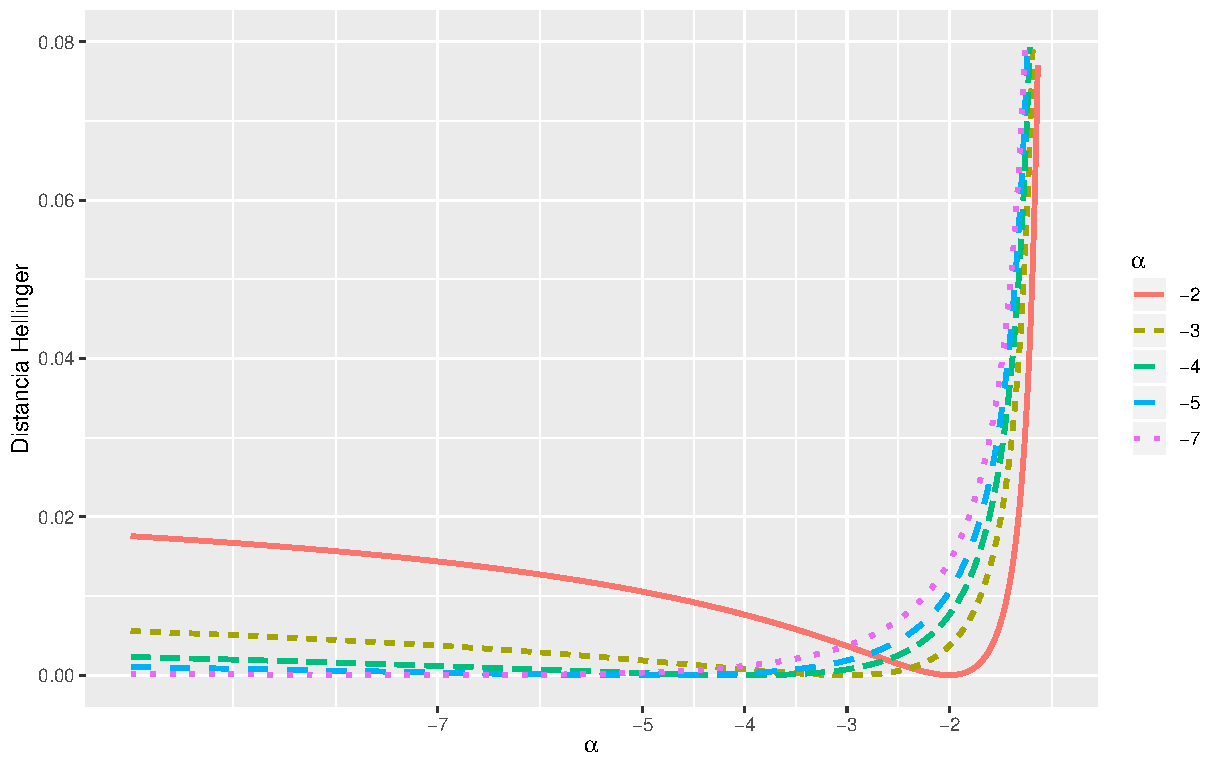
\includegraphics[width=.45\linewidth]{../../Figures/Tesis/Capitulo6/GraficoDHL1_v2.pdf}}
	\subfigure[Rényi]{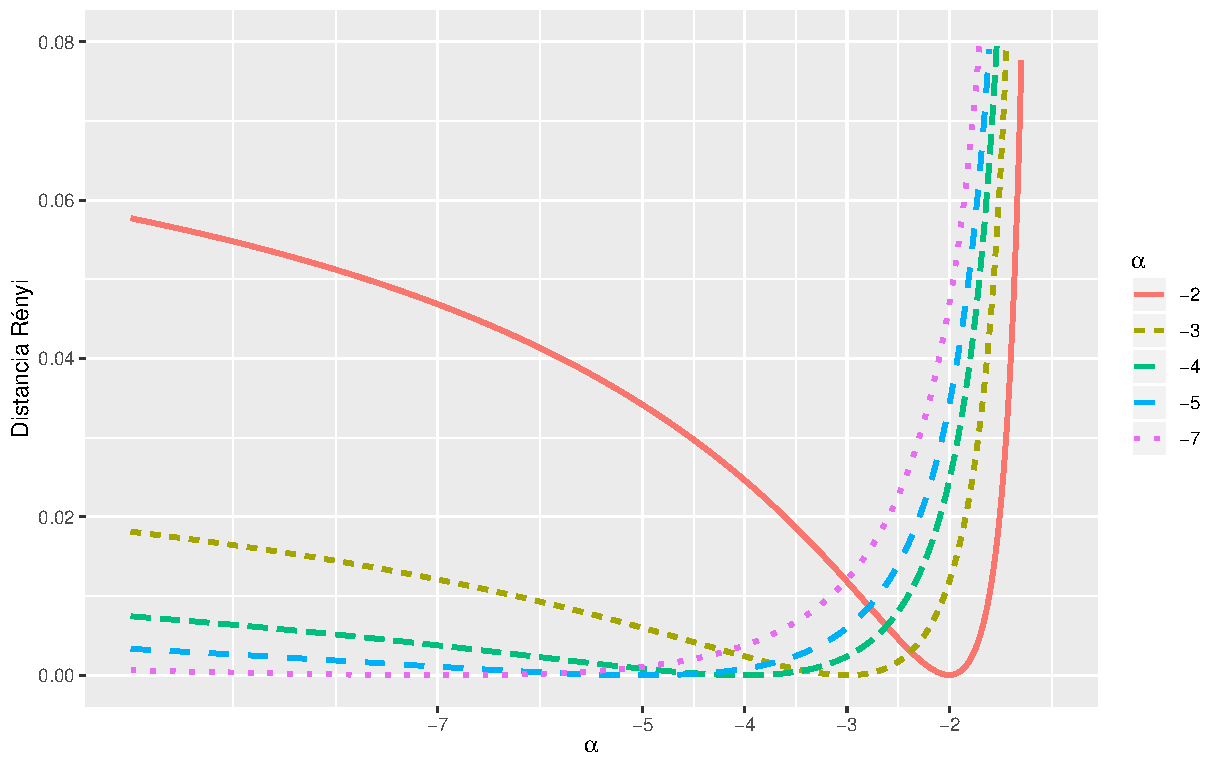
\includegraphics[width=.45\linewidth]{../../Figures/Tesis/Capitulo6/GraficoDRL1_v2.pdf}}
	\subfigure[Triangular]{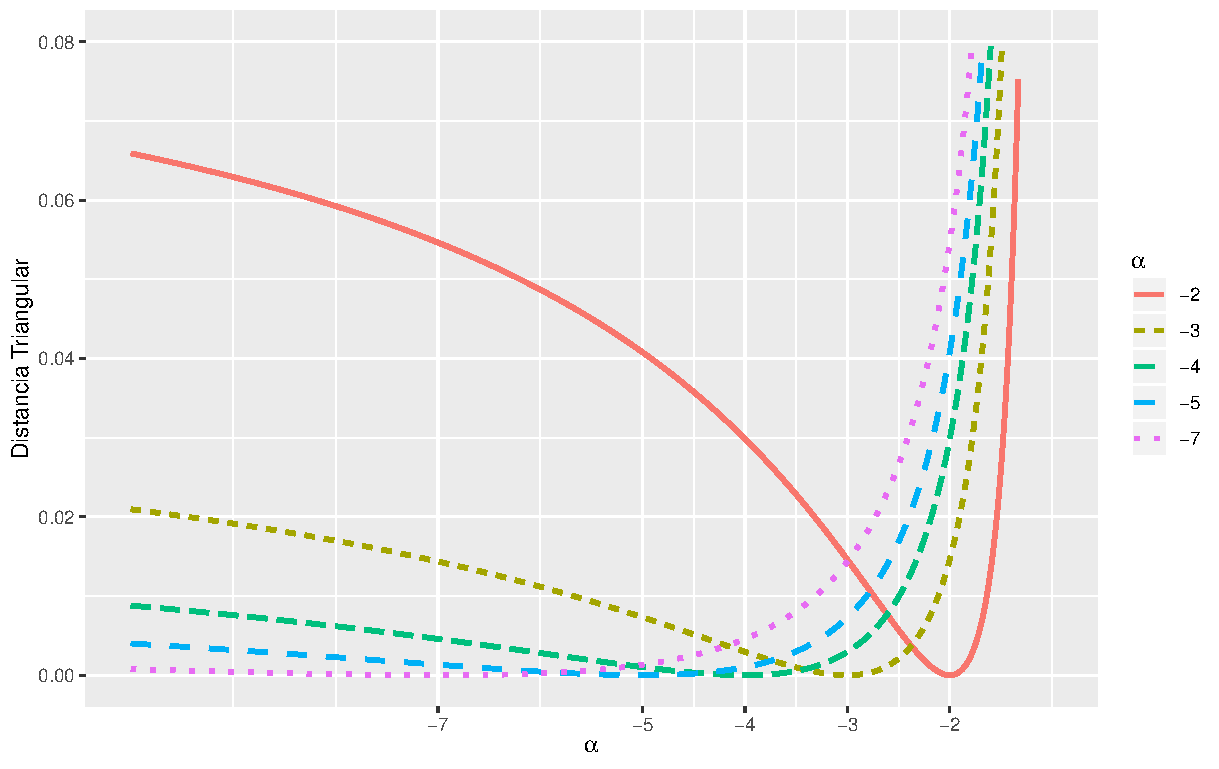
\includegraphics[width=.45\linewidth]{../../Figures/Tesis/Capitulo6/GraficoDTL1_v2.pdf}}
	\caption{\label{DistL1}\small Distancias Hellinger, Rényi y Triangular, $\alpha_0= -2,-3,-4,-5,-6,-7$ y $L=1$.}
\end{figure}


\begin{figure}[h!]
	\centering    
	\subfigure[Hellinger]{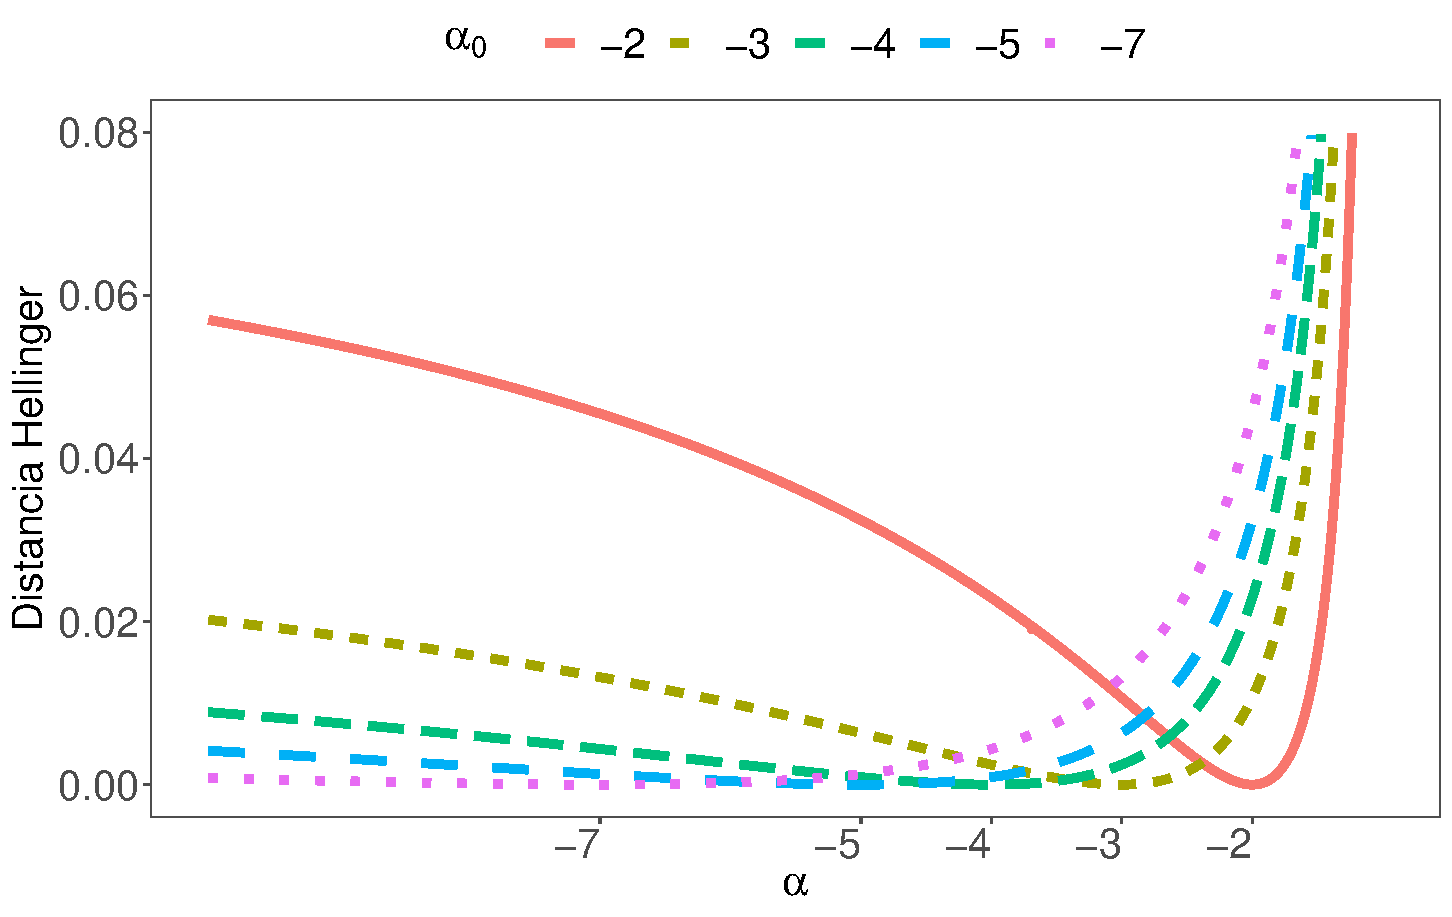
\includegraphics[width=.42\linewidth]{../../Figures/Tesis/Capitulo6/GraficoDHL3_v2.pdf}}
	\subfigure[Rényi]{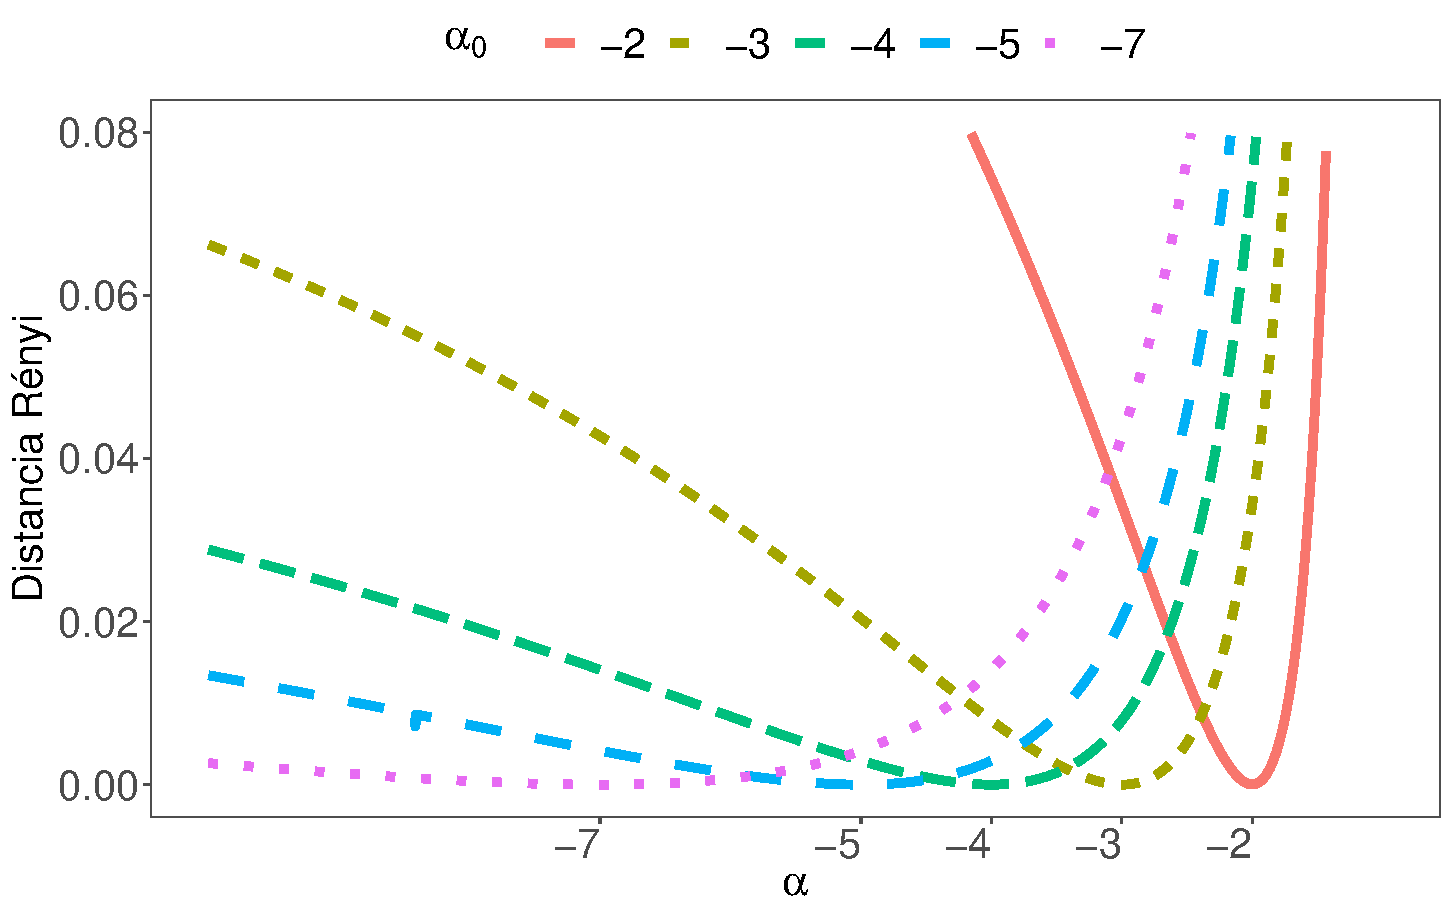
\includegraphics[width=.42\linewidth]{../../Figures/Tesis/Capitulo6/GraficoDRL3_v2.pdf}}
	\subfigure[Triangular]{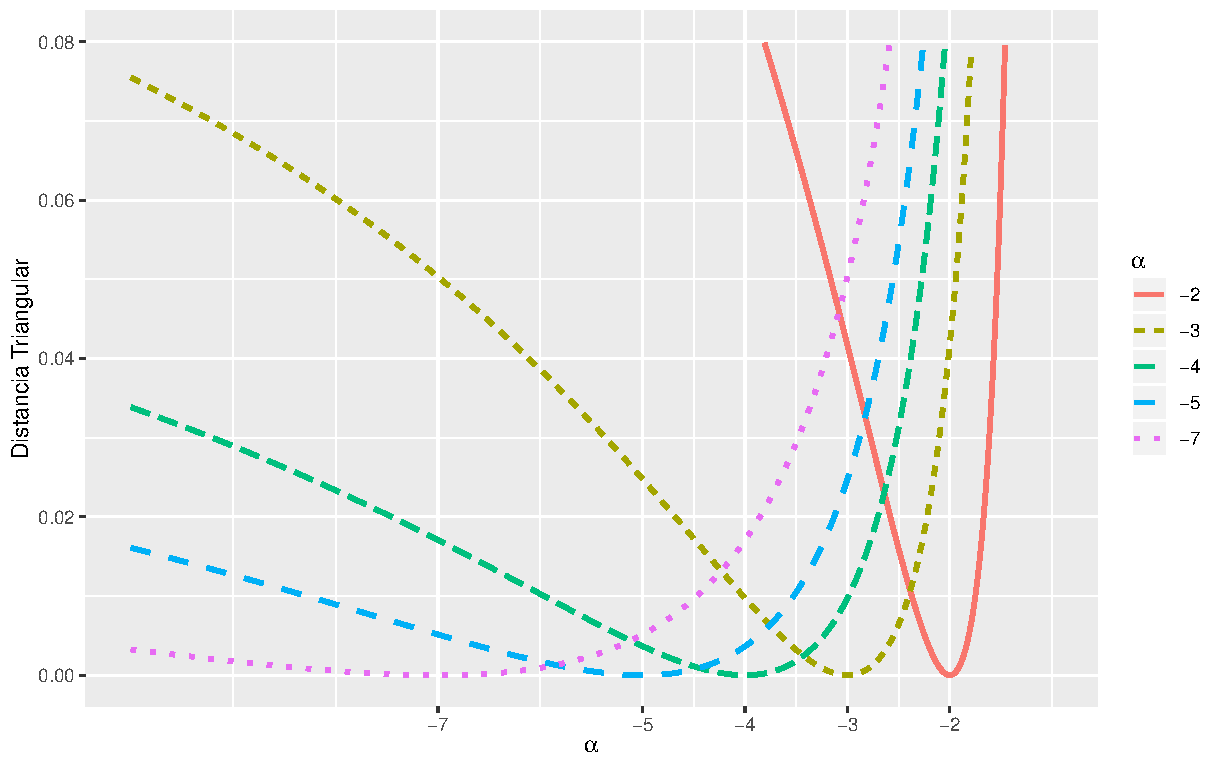
\includegraphics[width=.42\linewidth]{../../Figures/Tesis/Capitulo6/GraficoDTL3_v2.pdf}}
	\caption{\label{DistL3}\small Distancias Hellinger, Rényi y Triangular, $\alpha_0= -2,-3,-4,-5,-6,-7$ y $L=3$.}
\end{figure}

\begin{figure}[h!]
	\centering    
	\subfigure[Hellinger]{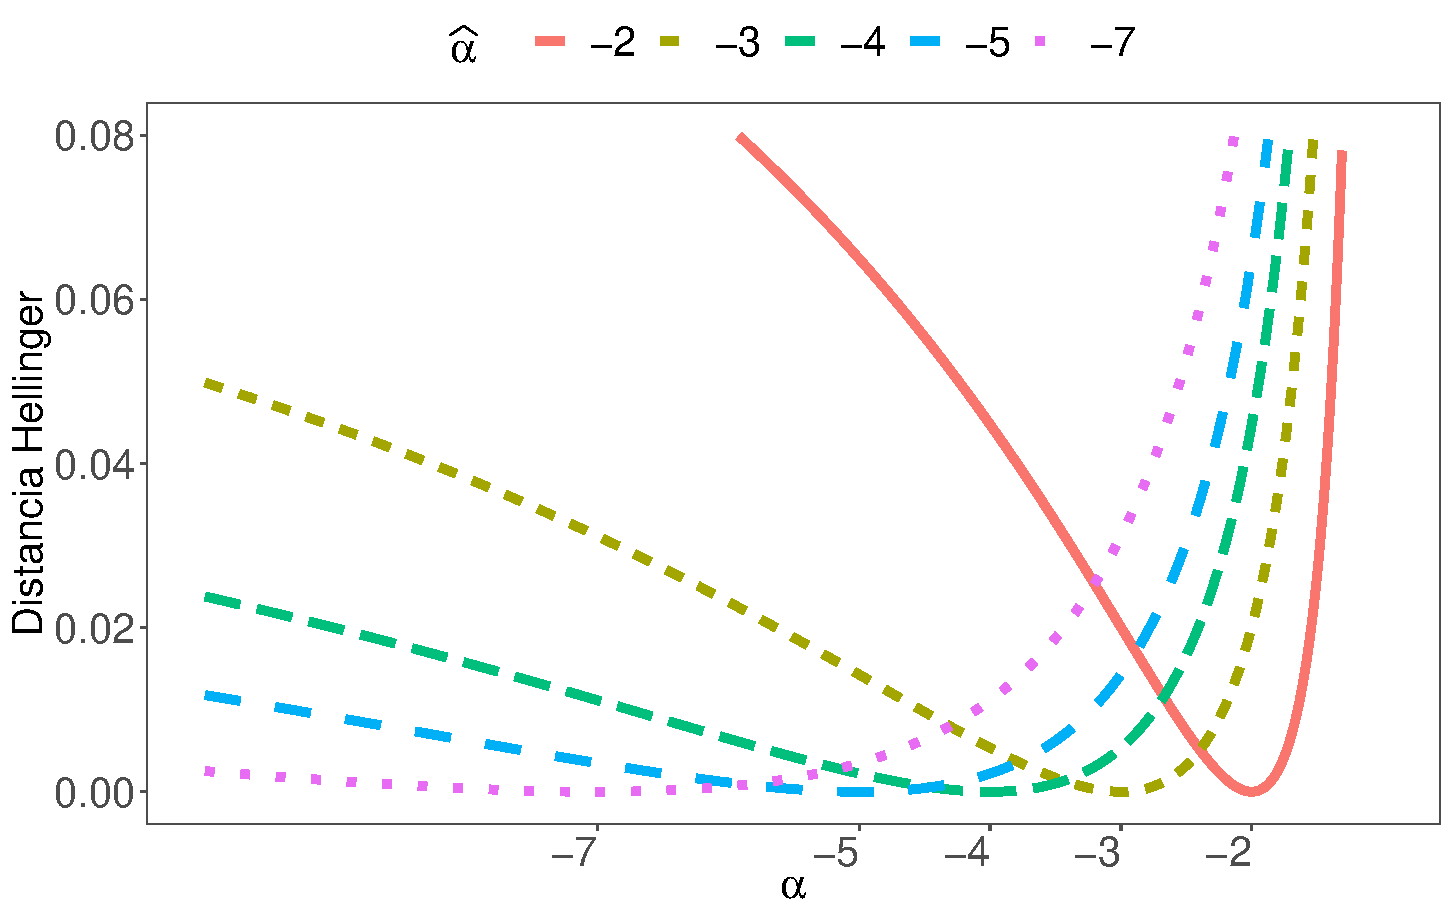
\includegraphics[width=.42\linewidth]{../../Figures/Tesis/Capitulo6/GraficoDHL8_v2.pdf}}
	\subfigure[Rényi]{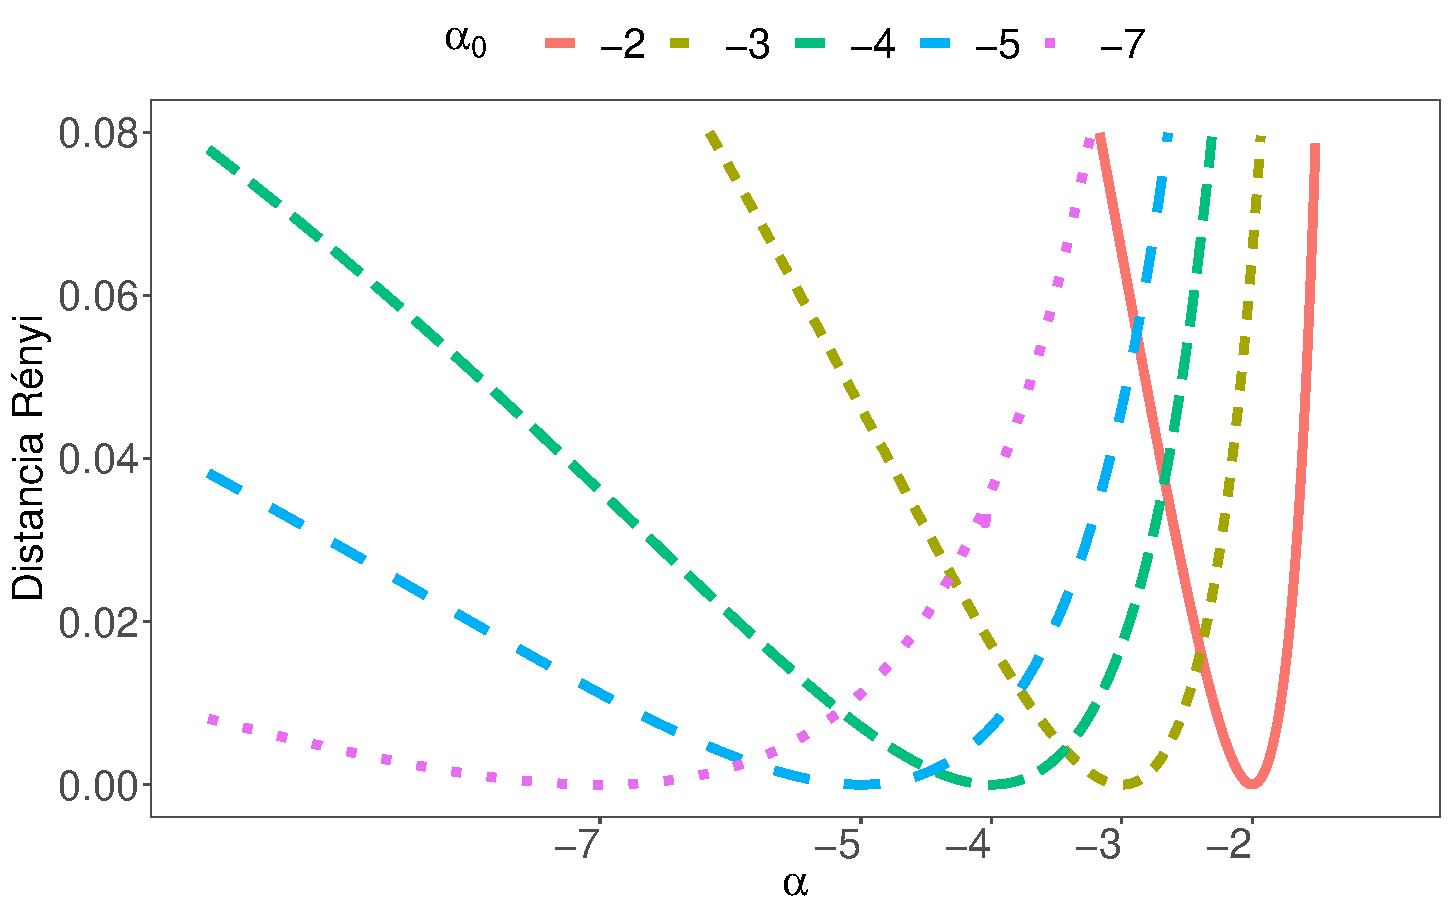
\includegraphics[width=.42\linewidth]{../../Figures/Tesis/Capitulo6/GraficoDRL8_v2.pdf}}
	\subfigure[Triangular]{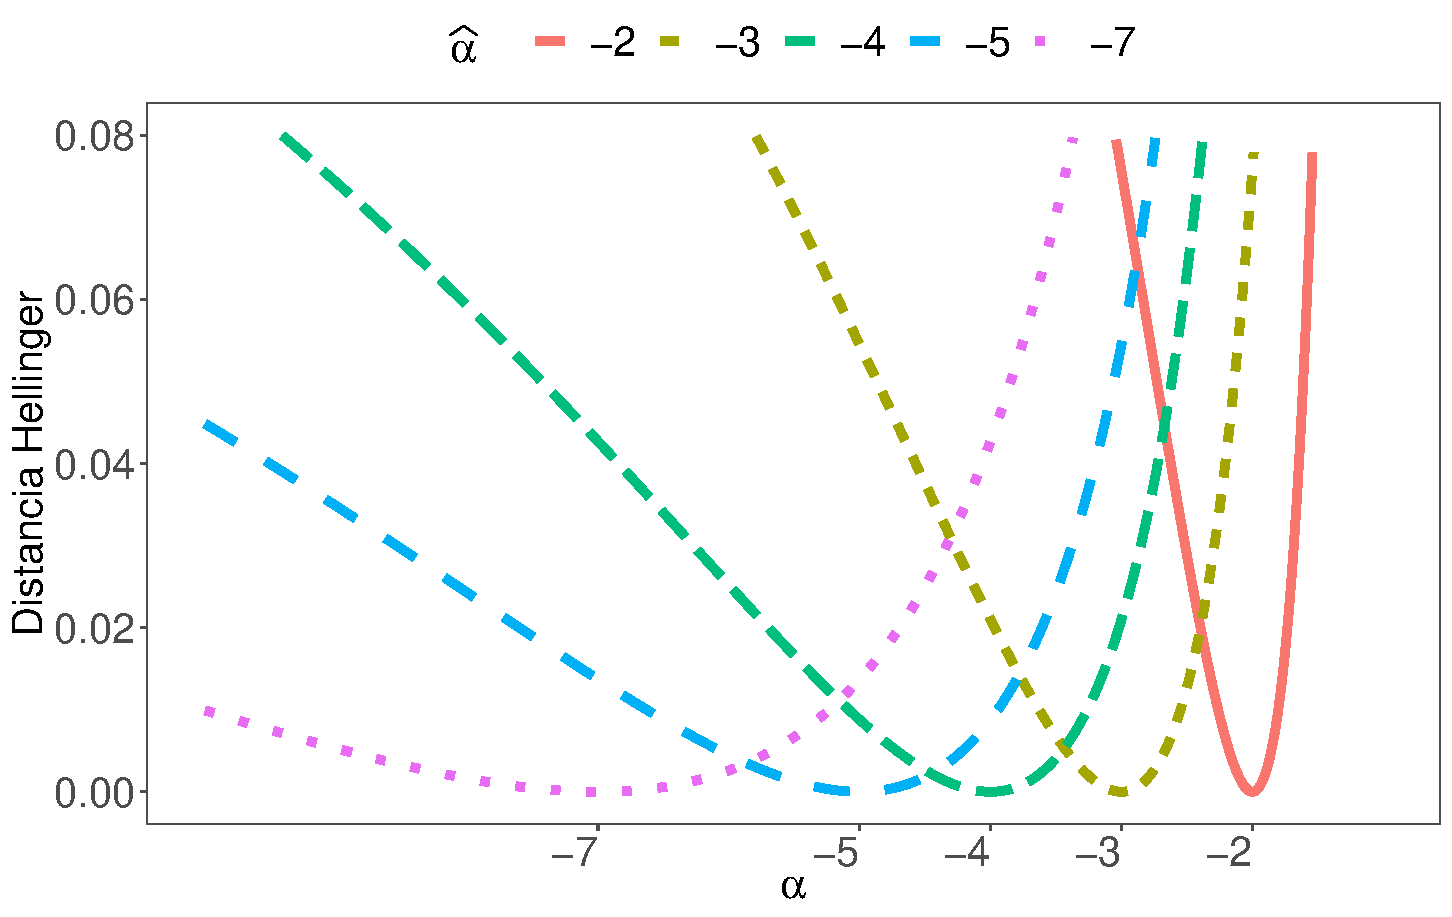
\includegraphics[width=.42\linewidth]{../../Figures/Tesis/Capitulo6/GraficoDTL8_v2.pdf}}
	\caption{\label{DistL8}\small Distancias Hellinger, Rényi y Triangular, $\alpha_0= -2,-3,-4,-5,-6,-7$ y $L=8$.}
\end{figure}

En estos gráficos se puede observar que, cuanto menor es el valor de $\alpha_0$ la curva se hace más plana. Por este motivo los métodos de optimización resultan más inestables y el mínimo es más difícil de encontrar en forma precisa. Se puede observar también que, a medida que aumenta el valor de $L$, esta situación se revierte y es posible encontrar el mínimo de una forma más eficiente. Recordemos que el número de looks representa la relación señal ruido, por lo tanto, cuanto mayor es el número de looks menor ruido presenta la imagen siendo $L=1$ el caso de mayor ruido. Se puede observar también que la distancia de Hellinger es la que resulta más plana en un entorno del mínimo, y que las distancias de Rényi y Triangular tienen un comportamiento similar.

Siguiendo en la búsqueda de la mejor distancia se realizaron simulaciones Monte Carlo para elegir la distancia estocástica que mejor performance tiene a la hora de estimar el parámetro de textura de la distribución $\mathcal{G}_I^0$. \citet{cassettiast2013} evaluaron dichas distancias estimando el parámetro de textura y  comparando la calidad de estos estimadores con el MV estimador en términos del sesgo y del error cuadrático medio. 

Se realizaron $1000$ replicaciones del experimento que consiste en generar muestras $Z_1, Z_2,\ldots,Z_n$ de variables aleatorias independientes e idénticamente distribuidas donde $Z_i \sim f_{\mathcal{G}_I^0(\alpha,\gamma^*,L)}$ donde el espacio paramétrico está formado por:

\begin{itemize}
	\item Textura: $\alpha=\{-1.5, -3, -5, -8\}$. Con estos valores se describen regiones extramadamente texturadas $(\alpha=-1.5)$, texturadas $(\alpha=\{-3,-5\})$ y homogéneas $(\alpha=-8)$. 
	\item Looks: $L=\{1,3,8\}$, para modelar varios niveles de procesamiento.
	\item Tamaño de muestra: $n=\{9, 25,49, 81,121,1000\}$. 
\end{itemize}

Como se mencionó anteriormente la elección de estos tamaños de muestra se basa en que muchos de los métodos de filtrado de imágenes o detección de bordes utilizan ventanas deslizantes para estimar los parámetros, las cuales suelen ser de tamaño $3 \times 3$,  $5 \times 5$, $7 \times 7$, $9 \times 9$ y  $11 \times 11$. Se consideró también una muestra de tamaño $n=1000$ para poder estudiar el comportamiento del estimador cuando el tamaño de muestra es grande. 

En cada replicación:
\begin{itemize}
	\item se estima la función de densidad subyacente $\widehat{f}$ utilizando histogramas junto con el método de Freedman Diaconis para elegir el ancho de banda $b$ dado por $b=2 \ \text{IQR}(z_1,\ldots,z_n) n^{-1/3}$ donde $\text{IQR}$ es el rango intercuartil.
	\item se calcula $\widehat{\alpha}= \mathop{\text{argmin}}\limits_{\alpha}d(f_{\mathcal{G}_I^0(\alpha,-\alpha-1,L)},\widehat{f})$ donde $d$ es alguna de las distancias estocásticas definidas en la sección~\ref{dist}.
\end{itemize} 

De esta manera se obtuvieron $1000$ valores estimados de $\alpha$, $\{\widehat{\alpha}_1, \dots, \widehat{\alpha}_{1000}\}$. Con estos valores se estimó la esperanza, el sesgo y el error cuadrático medio que están definidos por:

\begin{itemize}
	\item $\overline{\widehat{\alpha}}=(1000)^{-1}{\sum_{i=1}^{1000}{\widehat{\alpha}_i}}$
	\item $\widehat{B}(\widehat\alpha) = \overline{\widehat\alpha}- \alpha$
	\item $\widehat{\operatorname{\text{ECM}}}=({1000})^{-1}{\sum_{i=1}^{1000}{(\widehat{\alpha}_i-\alpha)^2}}$
\end{itemize}


Las figuras~\ref{ASTalfaL1},~\ref{ASTalfaL2} y~\ref{ASTalfaL3} muestran el sesgo del estimador propuesto para el parámetro de textura ($\widehat{\alpha}$) utilizando las distancias de Hellinger, Rényi, Triangular y también Máxima Verosimilitud, para distintos tamaños de muestras $n$ y número de looks $L$. 
La línea recta azul representa el eje $x$. 

En las figuras~\ref{ASTecmL1},~\ref{ASTecmL2} y~\ref{ASTecmL3} se muestra el error cuadrático medio (ECM) estimado para las mismas combinaciones de parámetros. Los resultados se muestran en escala semilogarítmica para su mejor comprensión visual.
Cabe señalar que la minimización se realizó recorriendo un rango de valores de alfa variando entre $-10$ y $-1$ con paso  $0.1$. 


%Se grafica también el intervalo de confianza de nivel aproximado $95\%$ para cada una de las estimaciones realizadas. Se utilizó el método del percentil que está en descripto \citet{Buckland1983}. Este método consiste en utilizar como límites superior e inferior del intervalo de confianza a los percentiles $(\alpha/2) 100\%$ y $(1-\alpha/2) 100\%$ de la distribución de $\widehat{\alpha}$ obtenida con las estimaciones en cada una de las muestas generadas. Este método fue evaluado por \citet{Buckland1983} en el caso donde la distribución subyacente es una exponencial donde falla la simetría de la distribución. El autor muestra que este intervalo tiene un mejor desempeño que el intervalo de confianza utilizando el método de aproximación normal. El método de percentiles se aplica en cada uno de los intervalos construidos en esta tesis.

Se grafica también el intervalo que tiene como límites superior e inferior a los percentiles $(\eta/2) 100\%$ y $(1-\eta/2) 100\%$ de la distribución de $\widehat{\alpha}$ obtenida con las estimaciones en cada una de las muestas generadas. En este caso hemos utilizado $\eta=0.05$. Este método fue evaluado por \citet{Buckland1983} en el caso donde la distribución subyacente es una exponencial que falla la simetría de la distribución. 

 Se puede observar que, en la mayoría de los casos estudiados, los estimadores del parámetro $\alpha$ utilizando distancia triangular y el método de Máxima Verosimilitud ($\widehat{\alpha}_{\text{\tiny{DT}}}$ y $\widehat{\alpha}_{\text{\tiny{MV}}}$ respectivamente) tienen un comportamiento similar en término de sesgo y ECM. Mientras que  el estimador utilizando las distancias de Hellinger y Rényi ($\widehat{\alpha}_{\text{\tiny{DH}}}$ y $\widehat{\alpha}_{\text{\tiny{DR}}}$ respectivamente) tienen una performance parecida. 
 
 En el gráfico de $L=1$ se observa que las distancias de Hellinger y Rényi muestran mayor ECM para tamaños de muestra mayores que $9$, salvo para zonas homogéneas donde el ECM es similar en todas las distancias estudiadas. Asimismo estas distancias muestran un mayor sesgo para muestras grandes.

Para el caso de $L=3$ y $L=8$ vemos que, en algunos casos el $\widehat{\alpha}_{\text{\tiny{DT}}}$ mejora la performance del $\widehat{\alpha}_{\text{\tiny{MV}}}$. Se puede observar que las otras distancias presentan un sesgo y un ECM mayor para zonas texturadas y homogéneas. Asimismo, en estos gráficos se observa que los métodos de minimización de distancias poseen menor ECM para valores grandes del número de looks. 

\begin{figure}[htb]
	\centering    
	\subfigure[\small $\widehat{\text{Sesgo}}$]{\label{ASTalfaL1}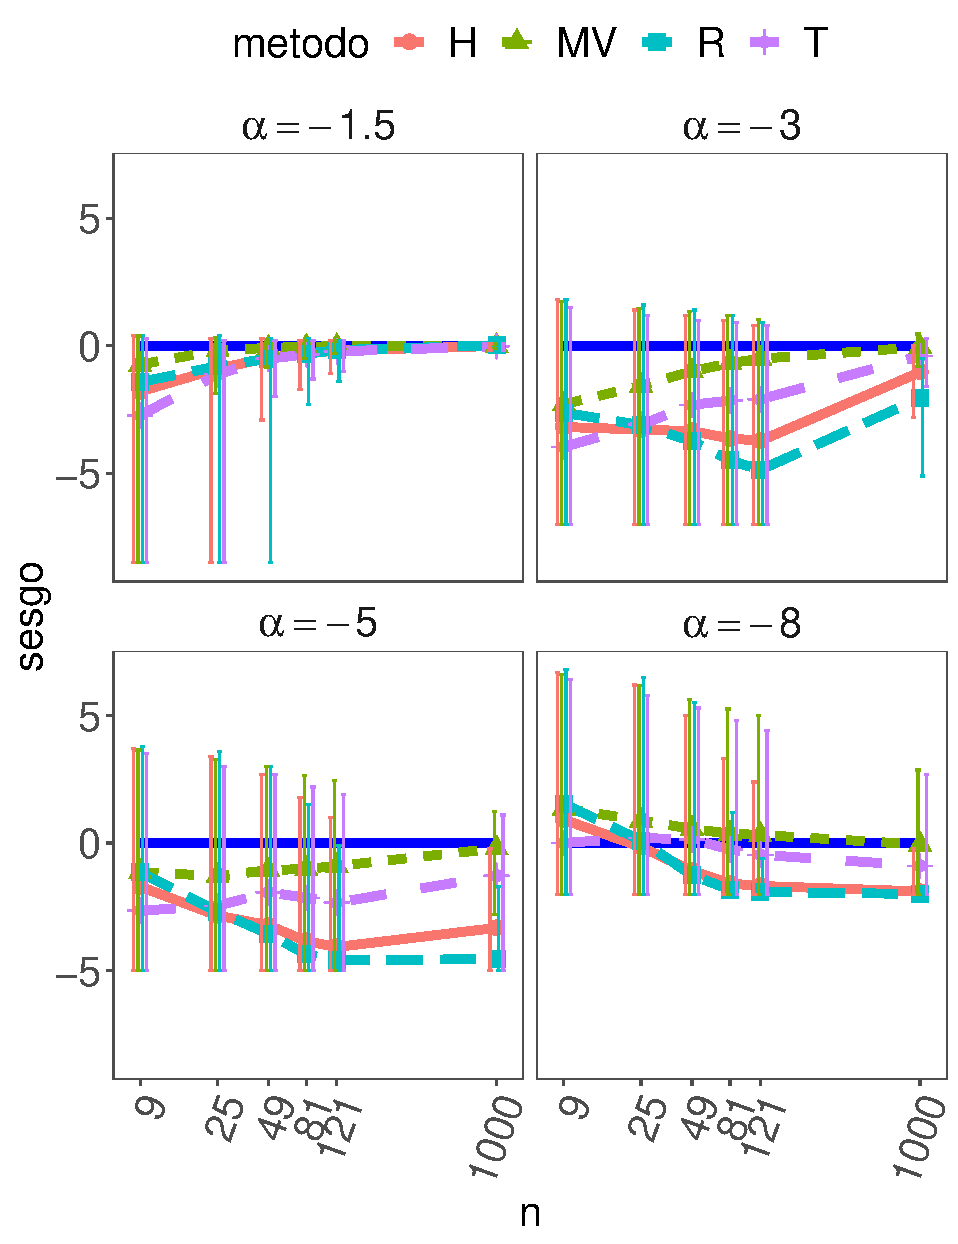
\includegraphics[width=.48\linewidth]{../../Figures/Tesis/Capitulo6/SesgoASTBarrasError_L1ypercentil.pdf}}
	\subfigure[\small $\widehat{\text{ECM}}$]{\label{ASTecmL1}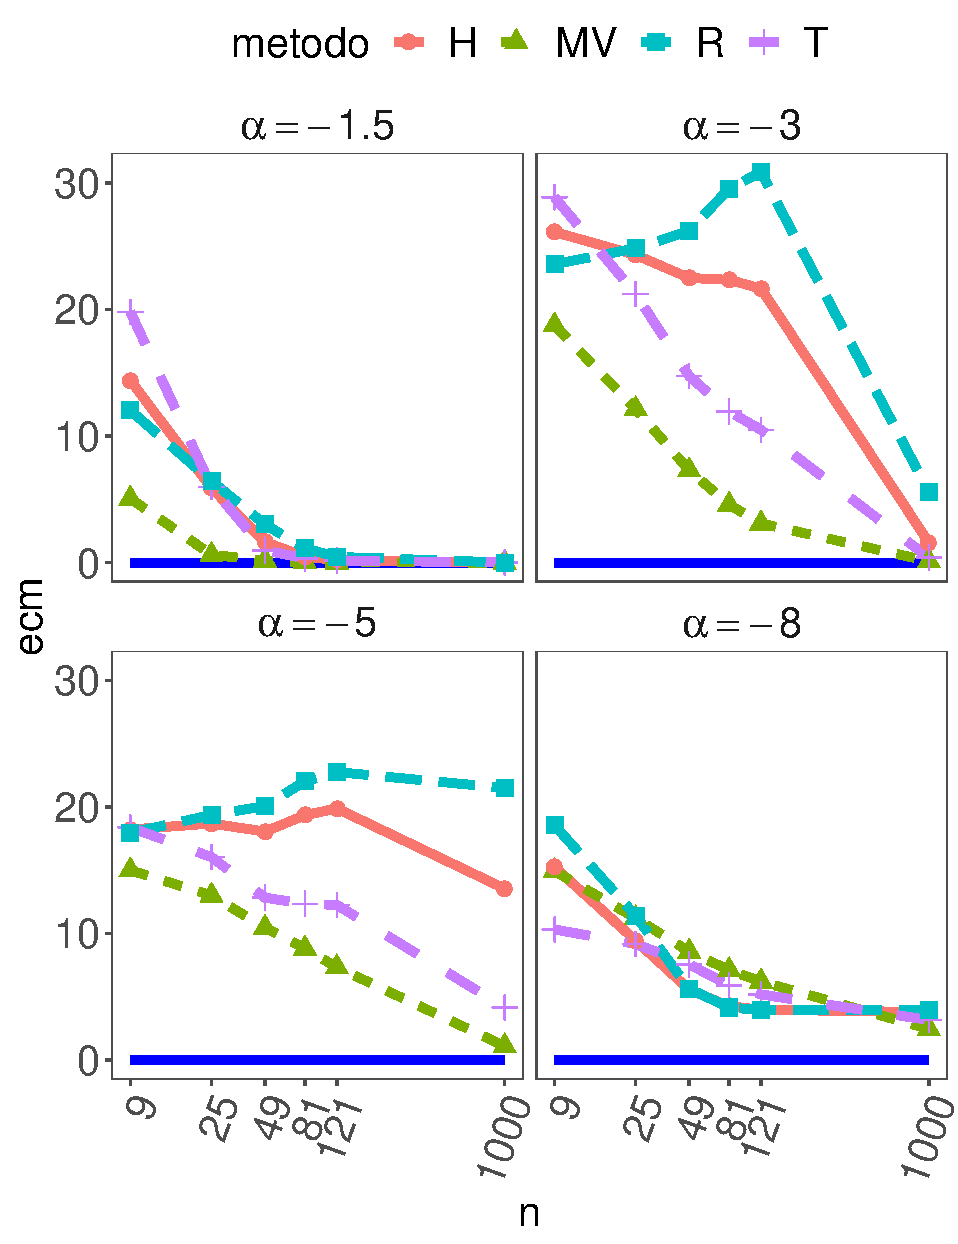
\includegraphics[width=.48\linewidth]{../../Figures/Tesis/Capitulo6/ECMASTBarrasError_L1ypercentil.pdf}}
	\caption{\small $\widehat{\text{Sesgo}}$ y $\widehat{\text{ECM}}$ de $\widehat{\alpha}$, L=$1$.}
\end{figure}	
\begin{figure}[htb]
	\centering
	\subfigure[\small $\widehat{\text{Sesgo}}$]{\label{ASTalfaL2}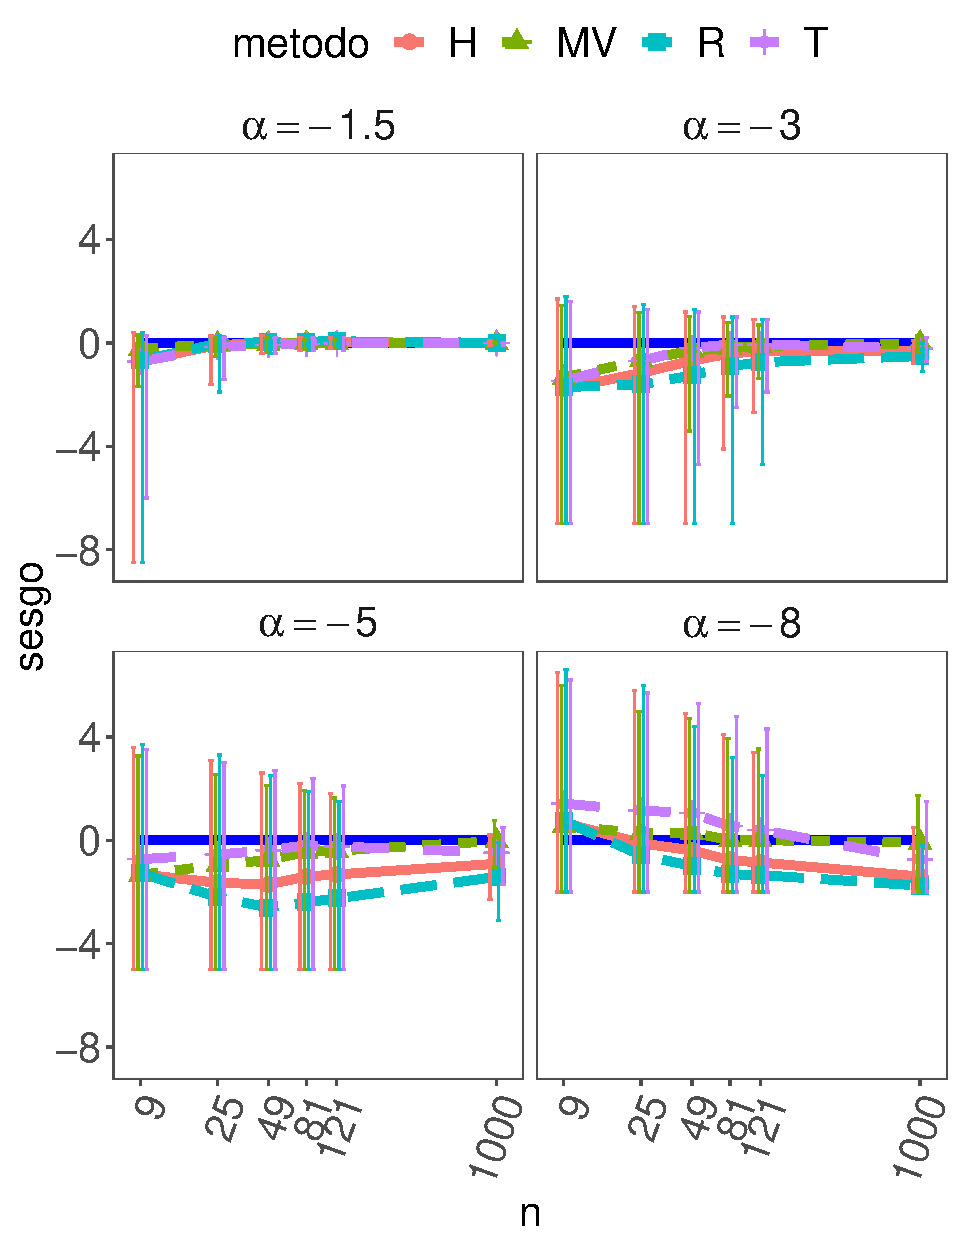
\includegraphics[width=.48\linewidth]{../../Figures/Tesis/Capitulo6/SesgoASTBarrasError_L3ypercentil.pdf}}
	\subfigure[\small $\widehat{\text{ECM}}$]{\label{ASTecmL2}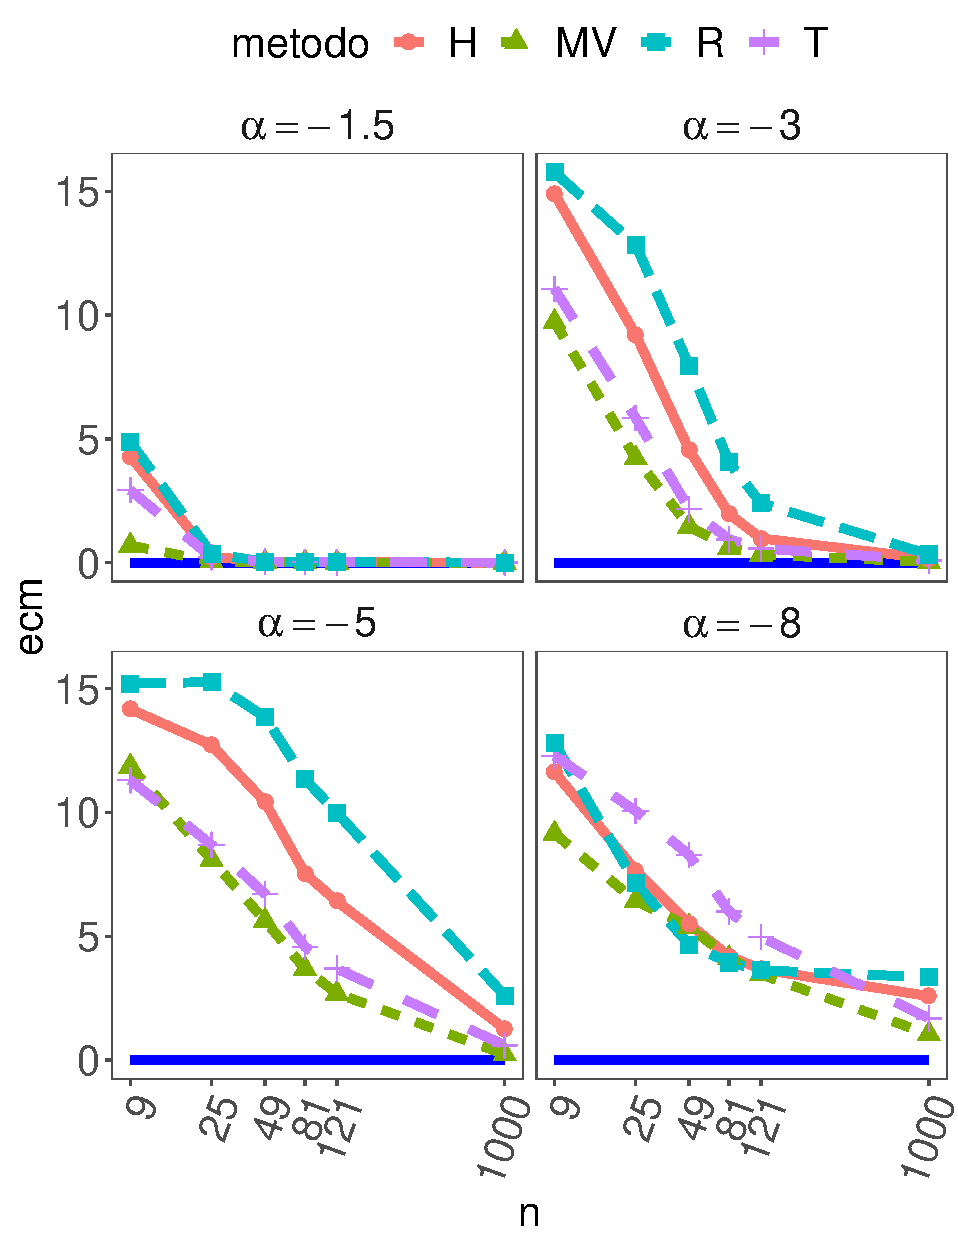
\includegraphics[width=.48\linewidth]{../../Figures/Tesis/Capitulo6/ECMASTBarrasError_L3ypercentil.pdf}}
	\caption{\small $\widehat{\text{Sesgo}}$ y $\widehat{\text{ECM}}$ de $\widehat{\alpha}$, L=$3$.}
\end{figure}	
\begin{figure}[htb]
	\centering
	\subfigure[\small $\widehat{\text{Sesgo}}$]{\label{ASTalfaL3}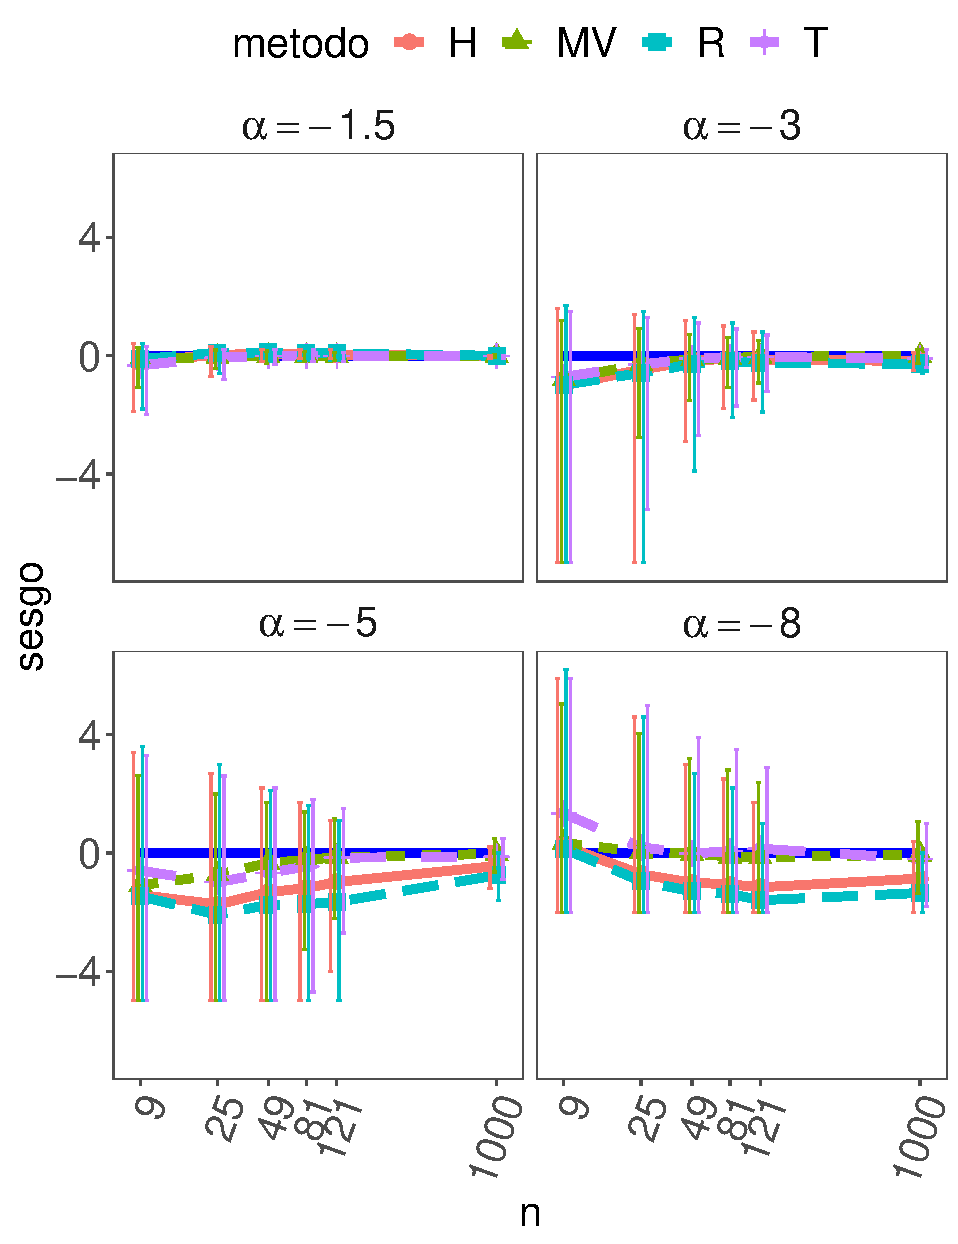
\includegraphics[width=.48\linewidth]{../../Figures/Tesis/Capitulo6/SesgoASTBarrasError_L8ypercentil.pdf}}
	\subfigure[\small $\widehat{\text{ECM}}$]{\label{ASTecmL3}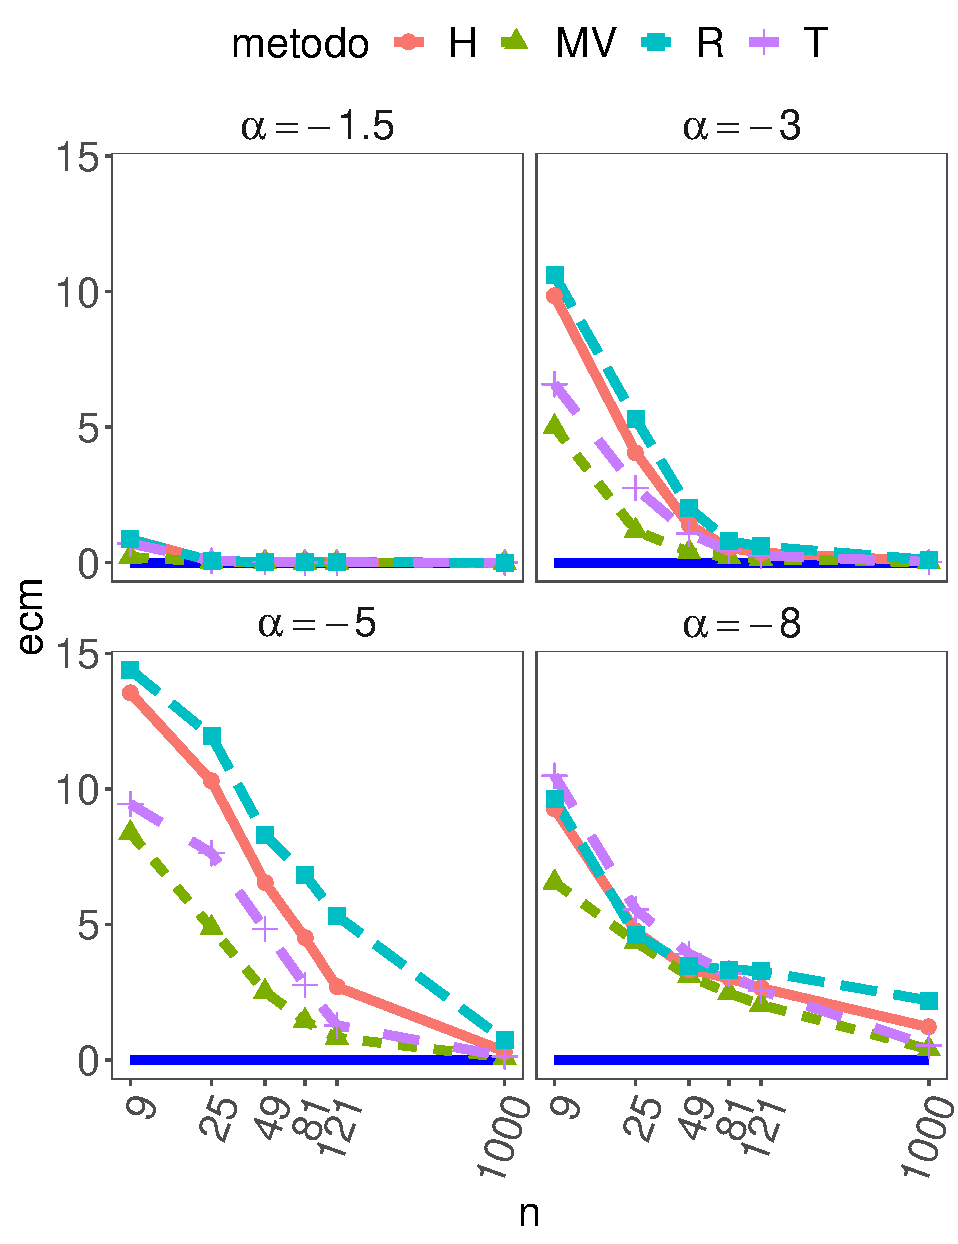
\includegraphics[width=.48\linewidth]{../../Figures/Tesis/Capitulo6/ECMASTBarrasError_L8ypercentil.pdf}}
	\caption{\small $\widehat{\text{Sesgo}}$ y $\widehat{\text{ECM}}$ de $\widehat{\alpha}$, L=$8$.}
\end{figure}

\citet{APSAR2013ParameterEstimationStochasticDistances} aplicaron la metodología anterior a una imagen SAR real. En este caso se utilizó una imagen E-SAR (\citet{Horn1996}) de un look de los alrededores de Munich, banda L, polarización HH, con $L=1$ en formato intensidad.
E-SAR es un sistema formado por sensores y algoritmos de procesamiento de señales desarrollado, entre otras instituciones, por el centro aeroespacial Deutsches Zentrum für Luft- und Raumfahrt German (DLR), un centro de investigación cuya área principal es la teledetección por microondas.  Este centro utiliza, mayoritariamente, sistemas SAR tanto en plataformas espaciales como aerotransportadas. El compromiso de la institución en los proyectos internacionales ERS-1 y SIR-100 / X-SAR dio origen a los conocidos sistemas aerotransportados SAR y E-SAR. 
%E-SAR opera en las bandas de frecuencia 4, x, C-, L- y P-banda, por lo tanto, cubre un rango de longitudes de onda de 3 a 85 cm. La polarización de la señal de radar es seleccionable, horizontal así como vertical. El modo polarimétrico se conmuta de impulso a impulso en la polarización (HH-HV-W-VH) -secuencia.

En las figuras~\ref{ImagenReales1} y~\ref{ImagenReales2} se muestran dos imágenes E-SAR, de un look, que se utilizaron para testear la performance de las distancias estudiadas y el MV estimador. En ambas figuras se aplicó el método para cada pixel, usando ventanas deslizantes de tamaño $7 \times 7$ y $3 \times 3$ respectivamente. Se puede observar que los resultados son prometedores ya que se analizó el caso de mayor ruido donde todos los métodos presentaron un comportamiento similar.


\begin{figure}[htb]
	\begin{minipage}[b]{0.45\linewidth} %Una minipágina que cubre la mitad de la página
		\centering
		\subfigure[\label{ImagenReales1} Imagen E-SAR, L=$1$.]{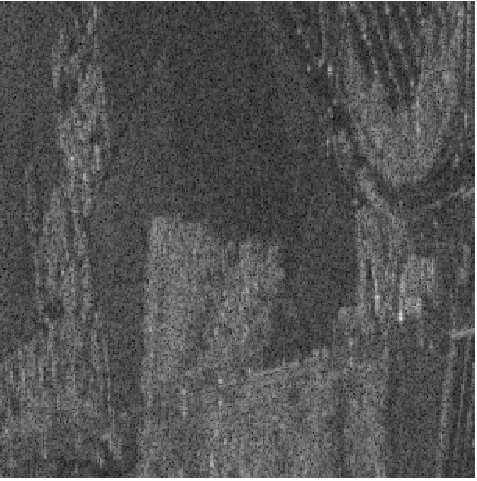
\includegraphics[width=.46\linewidth]{../../Figures/Tesis/Capitulo6/ImHorrible.pdf}}\\
		\subfigure[\label{Real1DH} Hellinger.]{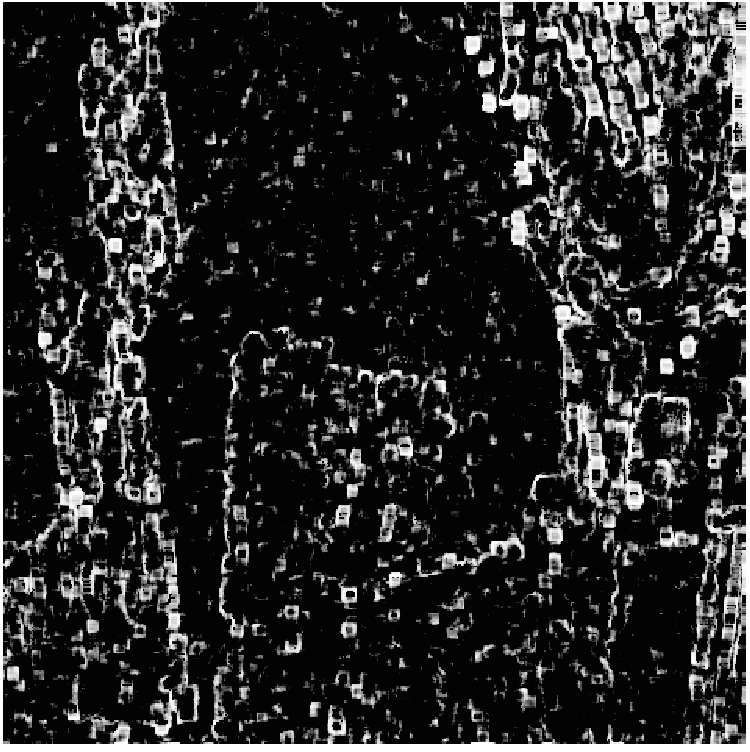
\includegraphics[width=.44\linewidth]{../../Figures/Tesis/Capitulo6/ImHorrible_DH7x7.pdf}}
		\subfigure[\label{Real1DR} R\'enyi, $\beta=0.8$.]{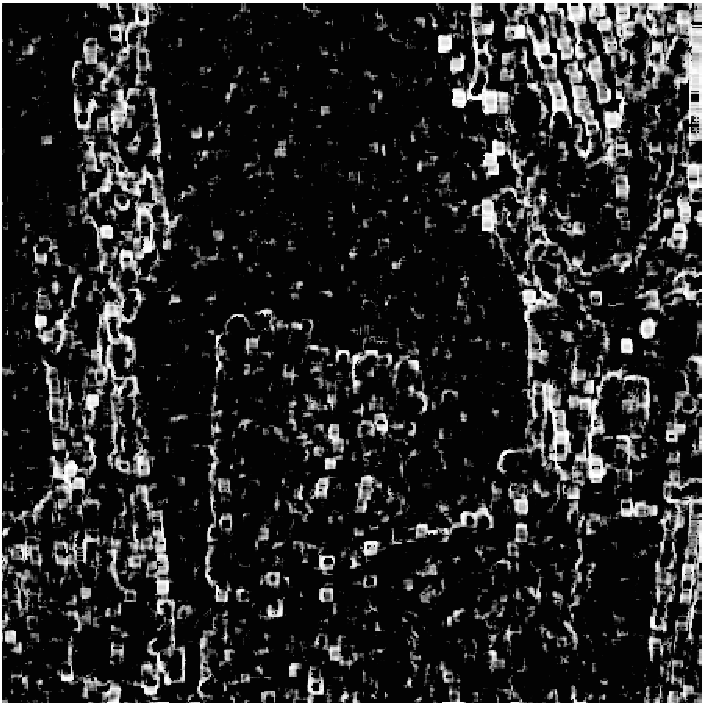
\includegraphics[width=.44\linewidth]{../../Figures/Tesis/Capitulo6/ImHorrible_DR7x7.pdf}}
		\subfigure[\label{Real1DT} Triangular.]{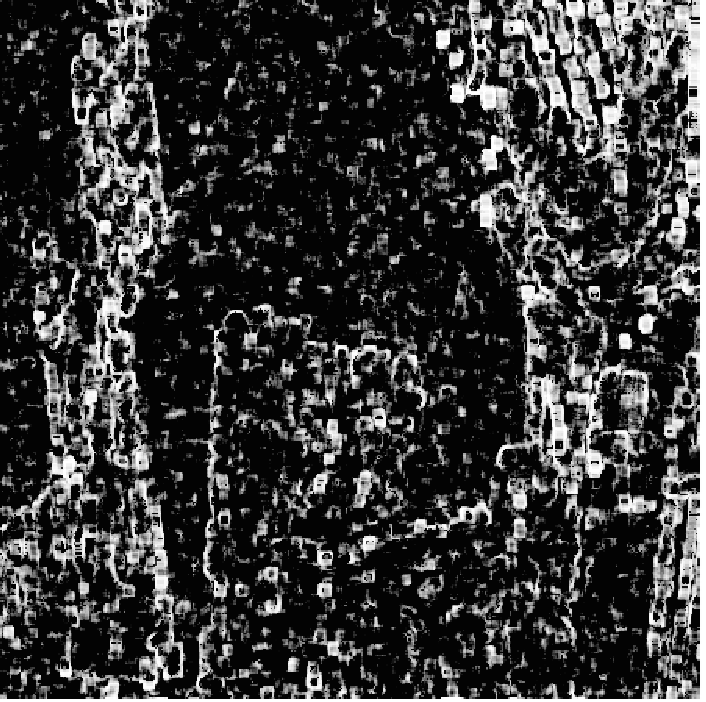
\includegraphics[width=.44\linewidth]{../../Figures/Tesis/Capitulo6/ImHorrible_DT7x7.pdf}}
		\subfigure[\label{Real1MV} MV.]{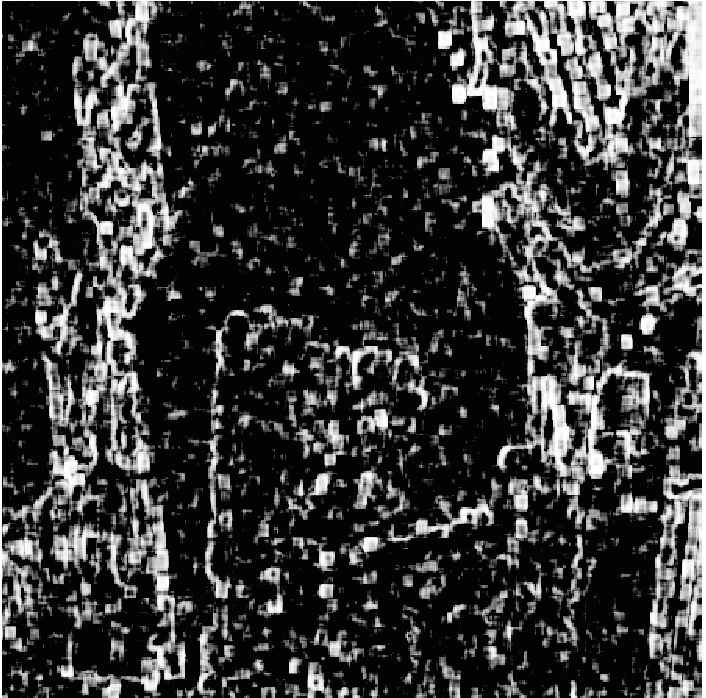
\includegraphics[width=.44\linewidth]{../../Figures/Tesis/Capitulo6/ImHorrible_MV7x7.pdf}}
		\caption{\small Resultado de estimar el parámetro $\alpha$ para cada pixel, usando ventanas deslizantes de tamaño $7\times 7$.}
	\end{minipage}
\hspace{0.3cm} % Si queremos tener un poco de espacio entre las dos figuras
	\begin{minipage}[b]{0.55\linewidth} %Una minipágina que cubre la mitad de la página
		\centering    
		\subfigure[\label{ImagenReales2} Imagen E-SAR, L=$1$.]{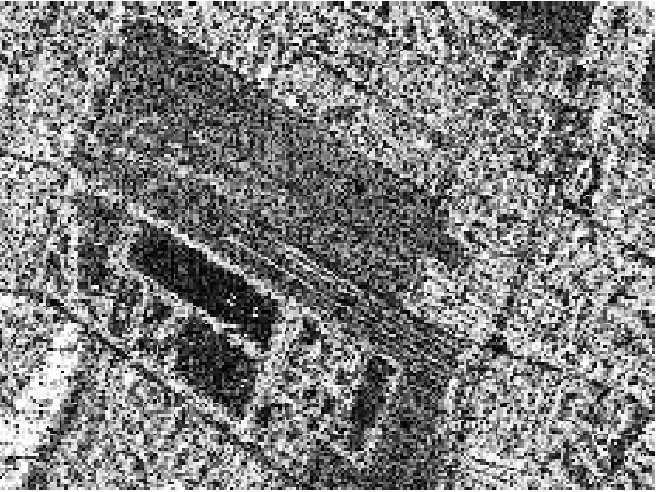
\includegraphics[width=.49\linewidth]{../../Figures/Tesis/Capitulo6/MunichCortadaBien.pdf}}\\
		\subfigure[\label{Real2DH} Hellinger.]{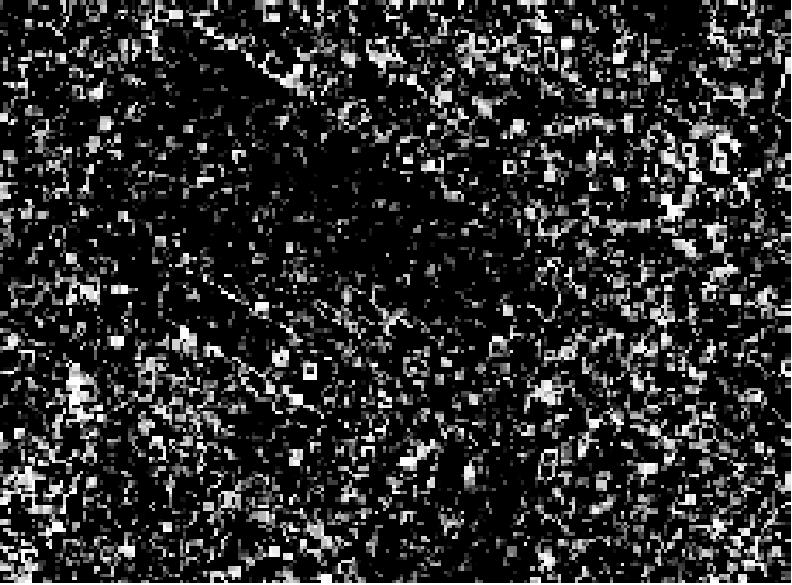
\includegraphics[width=.49\linewidth]{../../Figures/Tesis/Capitulo6/MunichCortada3regionesDH.pdf}}
		\subfigure[\label{Real2DR} R\'enyi, $\beta=0.8$.]{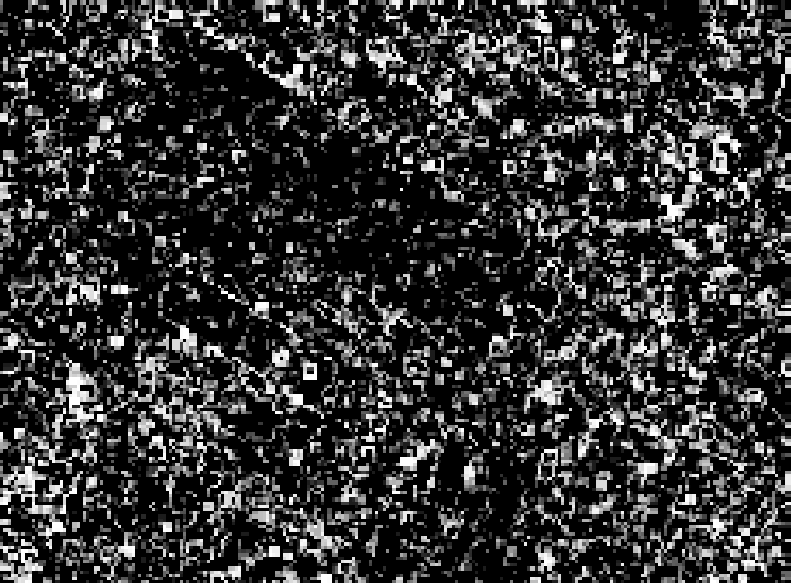
\includegraphics[width=.49\linewidth]{../../Figures/Tesis/Capitulo6/munichcortada3regionesR.pdf}}
		\subfigure[\label{Real2DT} Triangular.]{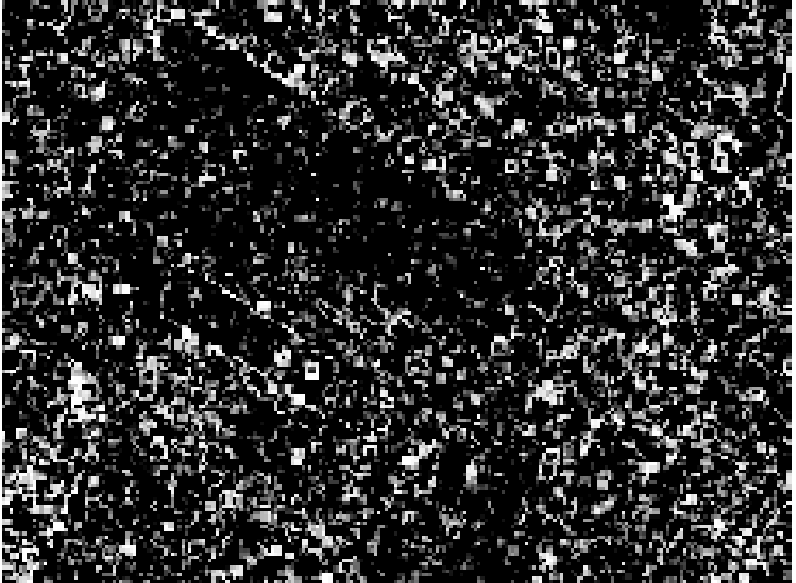
\includegraphics[width=.49\linewidth]{../../Figures/Tesis/Capitulo6/MunichCortada3regionesDT3x3.pdf}}
		\subfigure[\label{Real2MV} MV.]{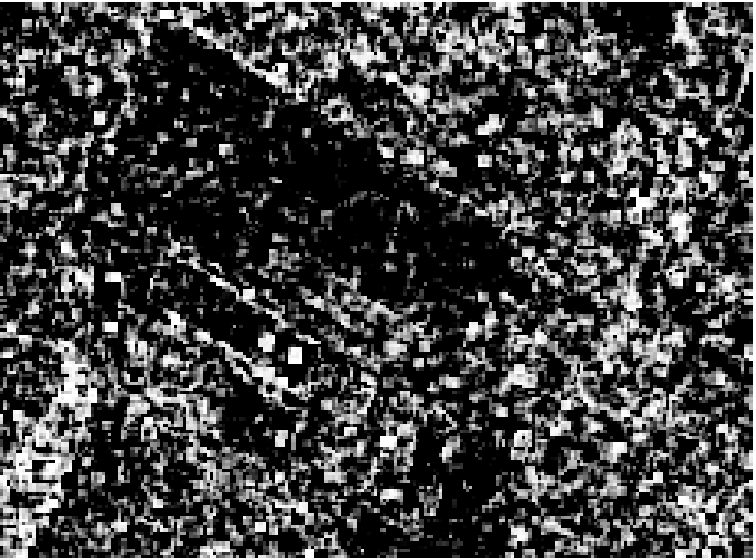
\includegraphics[width=.49\linewidth]{../../Figures/Tesis/Capitulo6/MunichCortada3RegionesMV.pdf}}
		\caption{\small Resultado de estimar el parámetro $\alpha$ para cada pixel, usando ventanas deslizantes de tamaño  $3\times 3$.}
\end{minipage}
\end{figure}
		


Por lo anteriormente expuesto, especialmente por el resulado de las simulaciones, elegimos la distancia Triangular para continuar con el estudio.


\section{Incorporando núcleos y evaluando robustez}
\label{jstar}

Como se mencionó en la sección~\ref{EligiendoDistancias}, en \citet{APSAR2013ParameterEstimationStochasticDistances} se compararon estimadores basados en la distancia de Hellinger, Bhattacharyya, Rényi y Triangular con el MV estimador. Se mostró que la distancia Triangular es la mejor opción para definir el MDE estimador. En ese trabajo se utilizaron histogramas para estimar la función de densidad subyacente. En \citet{gambini2015} %articulo que publicamos en la revista \textit{IEEE Journal of Selected Topics in Applied Earth Observations and Remote Sensing} 
presentamos mejoras con respecto a los resultados obtenidos en \citet{APSAR2013ParameterEstimationStochasticDistances} ya que: 
\begin{itemize}
	\item Se evaluó el impacto de la contaminación en la estimación de $\alpha$.
	\item Se emplearon núcleos asimétricos en lugar de histogramas para estimar la función de densidad subyacente.
	\item Se compararon los estimadores basados en la distancia Triangular ($\widehat{\alpha}_{\text{\tiny{DT}}}$) con el MV estimador ($\widehat{\alpha}_{\text{\tiny{MV}}}$), Momentos Fraccionales ($\widehat{\alpha}_{\text{\tiny{Mom12}}}$) y Logcumulantes ($\widehat{\alpha}_{\text{\tiny{LC}}}$). 
\end{itemize}

Los estimadores por momentos fraccionales han sido usados por \citet{Frery97,GambiniSC08} en el contexto de estimar el parámetro $\alpha$ para datos de amplitud. Para el caso de datos de intensidad, usando la relación $\gamma^*=-\alpha-1$ en la ecuación~\eqref{momento1medio} se tiene que, $\widehat{\alpha}_\text{Mom12}$ es el valor de $\alpha$ que resuelve la ecuación:

\begin{equation}
\frac{1}{n} \sum_{i=1}^n \sqrt{Z_i} -\sqrt{\frac{-\widehat\alpha_{\text{Mom12}}-1}{L}}\frac{\Gamma ( -\widehat\alpha_{\text{Mom12}}-{\frac{1}{2}} )}{ \Gamma (-\widehat\alpha_{\text{Mom12}}) }
\frac{\Gamma (L+{\frac{1}{2}} )}{\Gamma (L)}=0.
\label{estim_moment1_2_gI0}
\end{equation}
donde $Z_1,\ldots,Z_n$ es una muestra de variables aleatorias i.i.d proveniente del modelo $\mathcal{G}_I^0$.

En el capítulo~\ref{metodologia} se indicó que $\widehat{\alpha}_\text{MV}$ y $\widehat{\alpha}_\text{LC}$ son soluciones de las ecuaciones~\eqref{rootML} y~\eqref{eq:logm} respectivamente.

%En el modelo modelo multiplicativo para el retorno $Z=X \cdot Y$ con datos monopolarizados presentado en la sección XXX, la variable $Y$ que modela el ruido speckle obedece a una distribución $\Gamma(L,L)$, donde $L$ es el número de looks. La retrodisperción $X$ está modelada por una distribución Inversa Gaussiana Generalizada $\mathcal{N}^{-1}( \alpha ,\lambda ,\gamma )$ \citet{Frery97} donde,  para valores particulares de sus parámetros, se obtienen las distribuciones $\Gamma ( \alpha ,\lambda ) $,  $\Gamma ^{-1}( \alpha ,\gamma ) $ e $IG( \gamma ,\lambda ) $ (Gaussiana Inversa) originando que $Z$ esté modelado por las distribuciones $\mathcal{K}$, $\mathcal{G}_I^{0}$ y $\mathcal{G}^{H}$ respectivamente. La distribución $\mathcal{G}^{H}$ fue propuesta en \citet{harmoniceusar2000} y describe datos  polarimétricos con bastante precisión, aunque
%también se utiliza para imágenes monopolarizadas.

Como se indicó en la sección~\ref{NucleosAsimetricos}, dentro de los núcleos más estudiados se encuentran los núcleos $IG$, $\Gamma$ y LN. Estas distribuciones están presentes en el modelado de datos SAR, ya sea porque son propuestas para describir a la retrodispersión a partir del modelo multiplicativo, o bien porque fueron propuestas como modelo empírico. En el trabajo de \citet{gambini2015} estudiamos la perfomance del núcleo $IG$ para estimar la función de densidad subyacente ($\widehat f_\text{IG}$) en el contexto del MDE estimador y propusimos como estimador del parámetro de textura del modelo $\mathcal{G}_I^0$ a:

\begin{align}
\widehat{\alpha}_{\text{IG}}= \arg\min_{-20\leq \alpha \leq -1} d_{\text{T}}\big(f_{\mathcal{G}^{0}}(\alpha,\gamma^*, L ), \widehat f_\text{IG}\big),
\label{minimization}
\end{align}
donde $d_{\text{T}}$ es la distancia triangular definida en la ecuación~\eqref{triangular} y $\gamma^*=-\alpha-1$.  

Como es sabido, uno de los puntos importantes en estimación no paramétrica de la función de densidad es el ancho de banda. En esta oportunidad y, a través de estudios empíricos, se eligió un ancho de banda fijo $b=\frac{n^{-1/2}}{5}$.

%XXXXXXXXXXXXXXXXXXXXXXXXXXXXXXXXXXXXX

Ninguno de los problemas planteados para encontrar $\widehat{\alpha}$ tiene una solución explícita, por lo tanto apelamos a procedimientos numéricos acordes a cada estimador, para encontrar dichas soluciones. 

Respecto del estimador $\widehat{\alpha}_{{\text{\tiny{MV}}}}$ utilizamos la función $mle$ del software R-project que tiene incorporado el algoritmo L-BFGS-B, como se indica en \citet{Byrd1995}, para encontrar el óptimo de una función de una variable. Este algoritmo es un método de optimización tipo cuasi newton que admite restricciones de borde y, de acuerdo a \citet{Fei2014}, es ampliamente utilizado en computación gráfica y computación científica. Este algoritmo aproxima al método BFGS (Broyden, Fletcher, Goldfarb y Shanno) ya que no necesita calcular la matriz Hessiana sino que utiliza una apoximación de ella que se actualiza en cada iteración, usando solamente la función y su gradiente. 
Respecto del estimador $\widehat{\alpha}_{{\text{\tiny{LC}}}}$ y $\widehat{\alpha}_{{\text{\tiny{Mom12}}}}$ utilizamos la función $uniroot$ del mismo software que implementa el método de bisección para encontrar el cero de una función. En cuanto a la integración numérica presente se utilizó la función $\textit{adaptintegrate}$ del paquete $\textit{cubature}$ donde se particiona recursivamente el dominio de integración
en subdominios más pequeños, aplicando la misma regla de integración a cada uno, hasta que se logre la convergencia.

%Un problema que se presenta al momento de estimar el parámetro de textura es la falta de convergencia a una solución global, especialmente en el caso de muestras de pequeño tamaño. Frery et al. \citet{FreryCribariSouza:JASP:04} and Pianto and Cribari-Neto \citet{DealingMonotoneLikelihood} propusieron técnicas que tienen como objetivo aliviar este problema, a expensas de un costo computacional alto.

%Un problema que se presenta al momento de estimar el parámetro de textura utilizando las técnicas propuestas incluido ML y aquellos basados en momentos fraccionales \citet{Frery97} y  Logcumulantes \citet{MellinAnalysisPolSAR,BujorTrouveValetNicolas2004,khan2014} es la necesidad de contar con algoritmos iterativos para los cuales no hay garantía de convergencia a una solución global. Esta falta de convergencia sucede en general, en el caso de muestras de pequeño tamaño. Frery et al. \citet{FreryCribariSouza:JASP:04} and Pianto and Cribari-Neto \citet{DealingMonotoneLikelihood} propusieron técnicas que tienen como objetivo aliviar este problema, a expensas de un costo computacional alto.

%XXXXXXXXXXXXXXXXXXXXXXXXXXXXXXXXXXXXXXXX

En la figura~\ref{densidades} se muestra el gráfico de la densidad del modelo $\mathcal{G}_I^0$ para valores de $\alpha=\{-20,-25\}$, $\gamma=\gamma^*$, $L=\{3,8\}$. Se puede observar que estas densidades son muy similares ya que, como se indica en \citet{Frery99}, la distribución $\mathcal{G}_I^0$ converge en distribución a una $\Gamma(L,L)$ cuando $\alpha \longrightarrow -\infty$ y $\gamma=\gamma^*$. Por este motivo se plantea que $\alpha$ tome valores en el intervalo $[-20,-1]$ en cada método numérico empleado. 

\begin{figure}[H]
	\centering
	\subfigure[L=3]{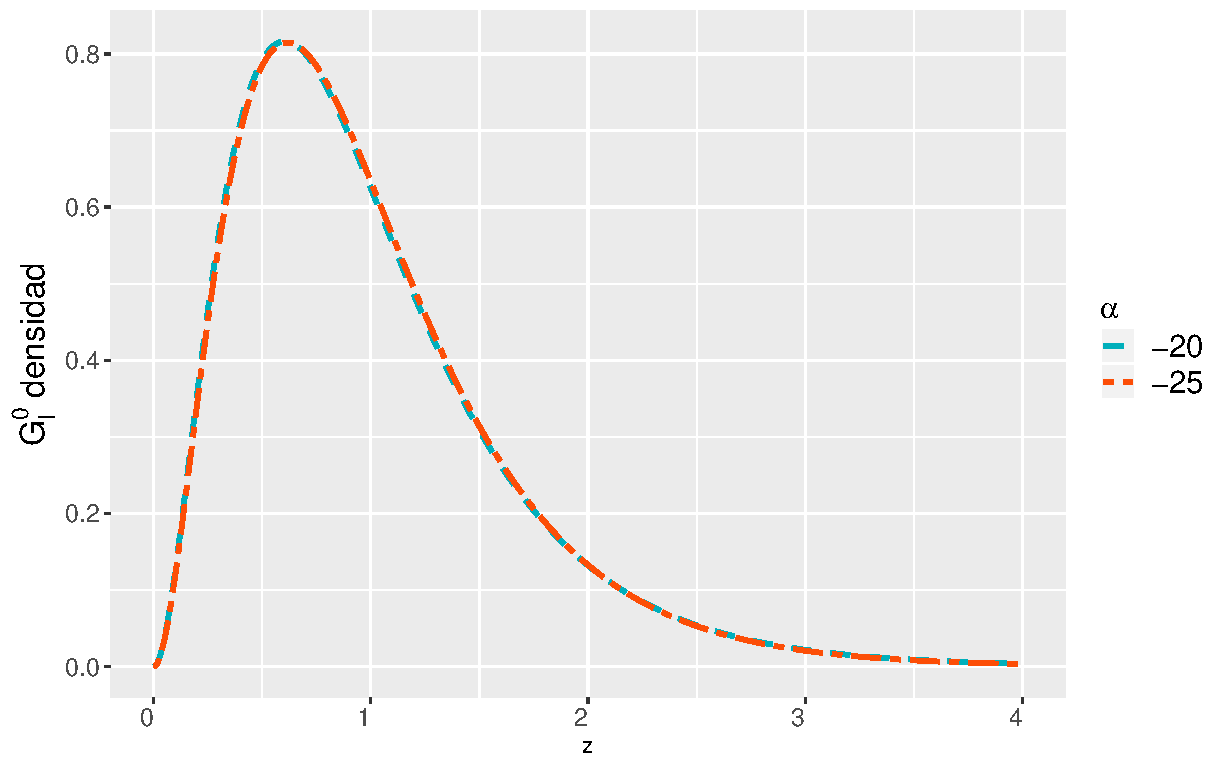
\includegraphics[width=.45\linewidth]{../../Figures/Tesis/Capitulo6/DensidadGI0L3.pdf}}
	\subfigure[L=8]{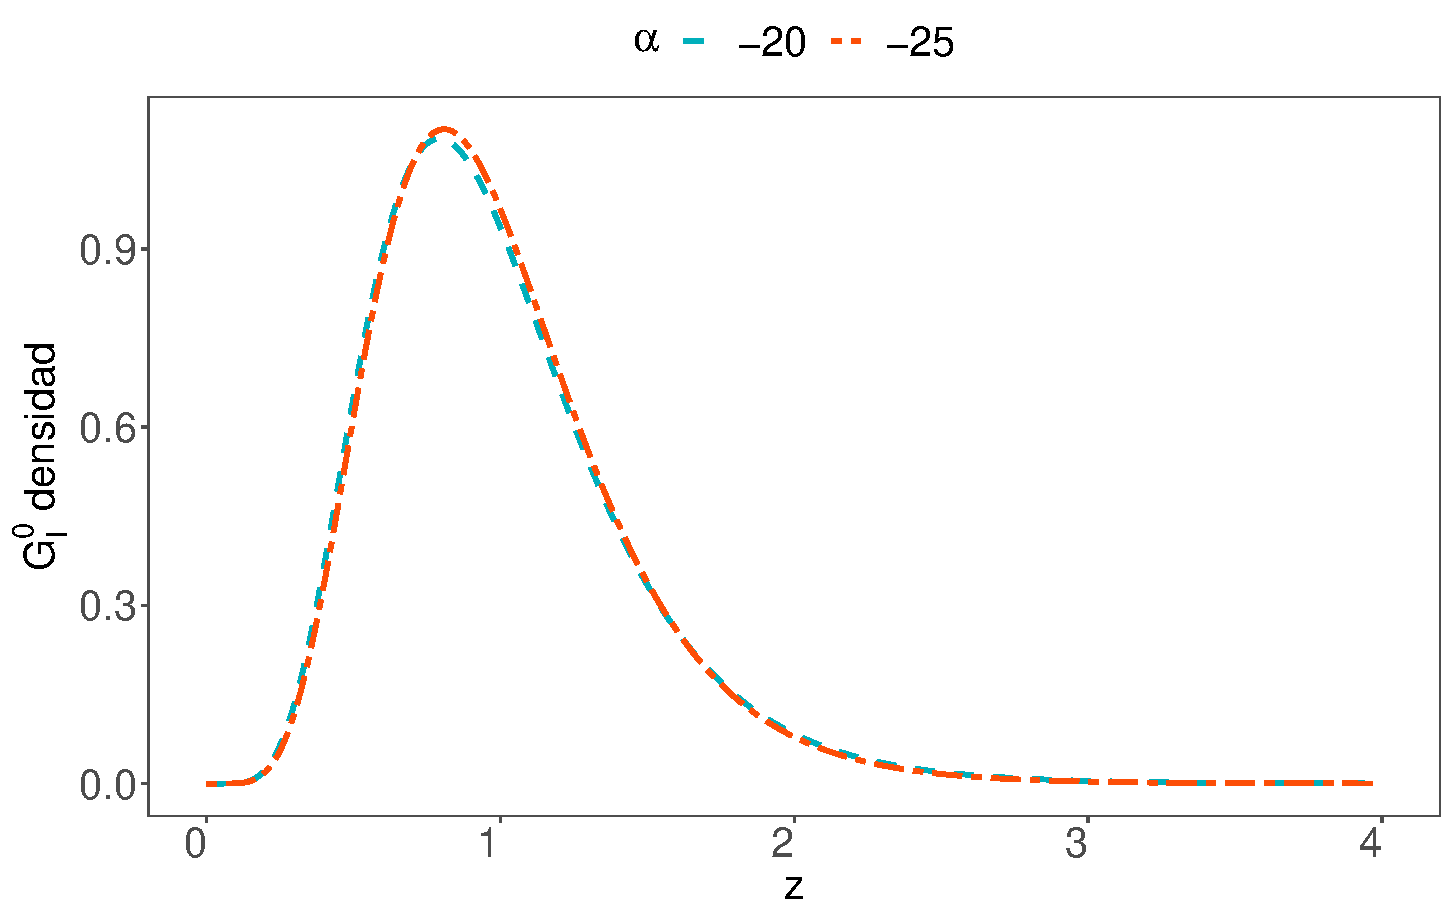
\includegraphics[width=.45\linewidth]{../../Figures/Tesis/Capitulo6/DensidadGI0L8.pdf}}
	\caption{\label{densidades}\small Densidad de $\mathcal{G}_I^0(\alpha,\gamma^*,L)$}
\end{figure}


Se realizó un experimento Monte Carlo para evaluar la performance de cada uno de los estimadores propuestos. El espacio parmétrico consiste en una grilla formada por:
\begin{itemize}
	\item tres valores de textura $\alpha=\{-1.5,-3,-5\}$. Los cuales representan áreas texturadas y extremadamente texturadas.
	\item tres niveles de procesamiento señal-ruido $L=\{1,3,8\}$.
	\item tamaños de muestra $n=\{9,25,49,81,121,1000\}$ compatibles con tamaños de ventana $3,\text{ }5,\text{ }7,\text{ }9$.
\end{itemize}

Se generaron $1000$ muestras para cada punto del espacio paramétrico, y se obtuvieron $\{\widehat{\alpha}_1, \dots, \widehat{\alpha}_{1000}\}$ estimaciones para cada una de estas combinaciones. De esta forma se estimaron, para cada uno de los estimadores estudiados
\begin{itemize}
	\label{ExperimentoMontecarlo}
	\item la media $\overline{\widehat{\alpha}}=(1000)^{-1}{\sum_{i=1}^{1000}{\widehat{\alpha}_i}}$,
	\item el sesgo  $\widehat{B}(\widehat\alpha) = \overline{\widehat\alpha}- \alpha$.
	 \item el error cuadrático medio $\widehat{\operatorname{ECM}}=({1000})^{-1}{\sum_{i=1}^{1000}{(\widehat{\alpha}_i-\alpha)^2}}$.
\end{itemize}
  
En las siguientes figuras ``MV'', ``DT'',``Mom12'' and ``LC'' denotarán al estimador basado en el método de Máxima Verosimilitud, distancia Triangular con núcleo IG, $\frac{1}{2}$-momento y Logcumulante, respectivamente. En el eje de las abscisas se grafica el tamaño muestral, el cual se presenta en escala semilogarítmica.

Las figuras~\ref{AlfasEstimadosJSTAR2013_L=1},~\ref{AlfasEstimadosJSTAR2013_L=3} y~\ref{AlfasEstimadosJSTAR2013_L=8} muestran el sesgo de $\widehat{\alpha}$ para datos sin contaminar y para diferentes valores de $n$ y $L$, la línea azul representa el eje $x$. Se puede observar que $\widehat{\alpha}_{\text{MV}}$ y $\widehat{\alpha}_{\text{DT}}$ tienen un comportamiento similar y un sesgo medio cercano a cero en la mayoría de los casos estudiados. Es notable el sesgo que presentan  $\widehat{\alpha}_{\text{LC}}$ y $\widehat{\alpha}_{\text{Mom12}}$ para $\alpha=-5$. Se puede observar también que $\widehat\alpha_{\text{MV}}$ tiende a subestimar al verdadero valor de $\alpha$, y que ningún método de estimación tiene el menor error cuadrático medio en todos los casos. El estimador $\widehat{\alpha}_{\text{Mom12}}$ es el que peor se comporta para zonas texturadas.

Todos los métodos presentan alta variabilidad para el caso de $L=1$, esta variabilidad disminuye a medida que aumenta el número de looks, incluso la longitud de los intervalos van disminuyendo a medida que aumenta el tamaño de muestra.
%Vasconcellos et al. \citet{VasconcellosFrerySilva:CompStat} computed a first order approximation of such bias for a closely related model, and our results are in agreement with those.
%The estimator based on the Triangular distance $\widehat\alpha_{\text T}$ compensates this bias.

\begin{figure}[H]
	\centering
	\subfigure[\label{AlfasEstimadosJSTAR2013_L=1}$\widehat{\text{Sesgo}}$]{\includegraphics[width=.48\linewidth]{../../Figures/Tesis/Capitulo6/GraficoSesgoJstar2013BarrasError_NoCont_L=1ypercentil.pdf}}
	\subfigure[\label{ECMEstimadosJSTAR2013_L=1}$\widehat{\text{ECM}}$]{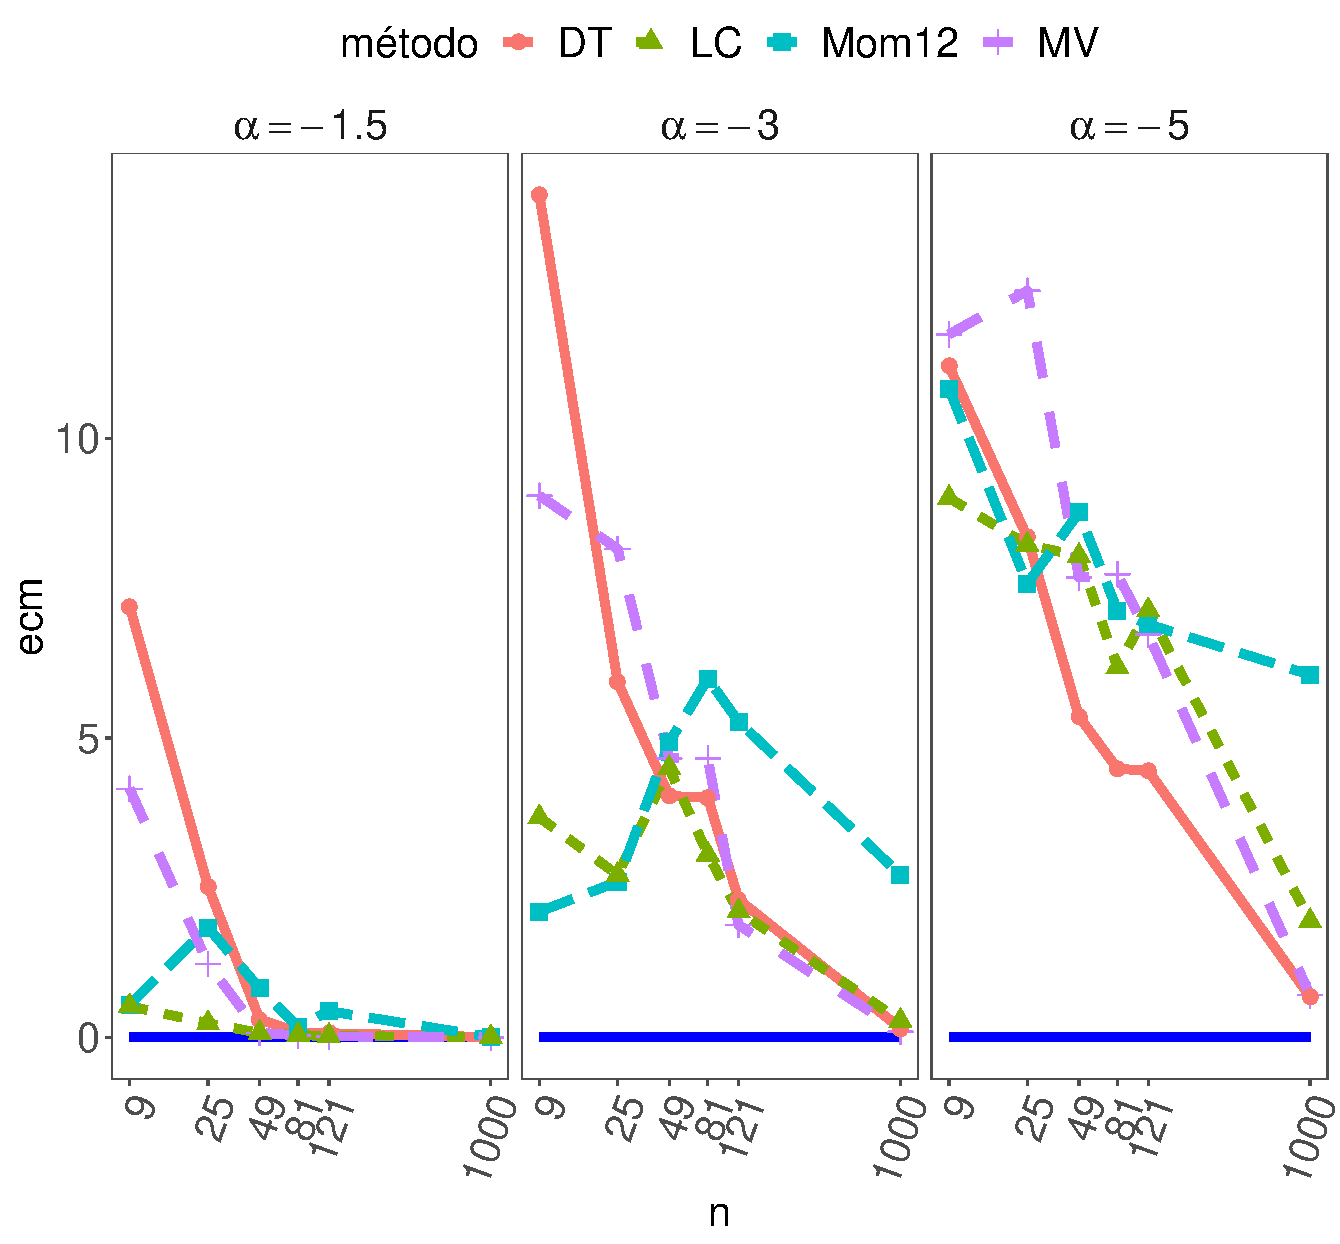
\includegraphics[width=.48\linewidth]{../../Figures/Tesis/Capitulo6/GraficoECMJstar2013BarrasError_NoCont_L=1ypercentil.pdf}}
%	\subfigure[\label{AlfasEstimadosJSTAR2013_L=3}$\widehat{\alpha}$, L=3]{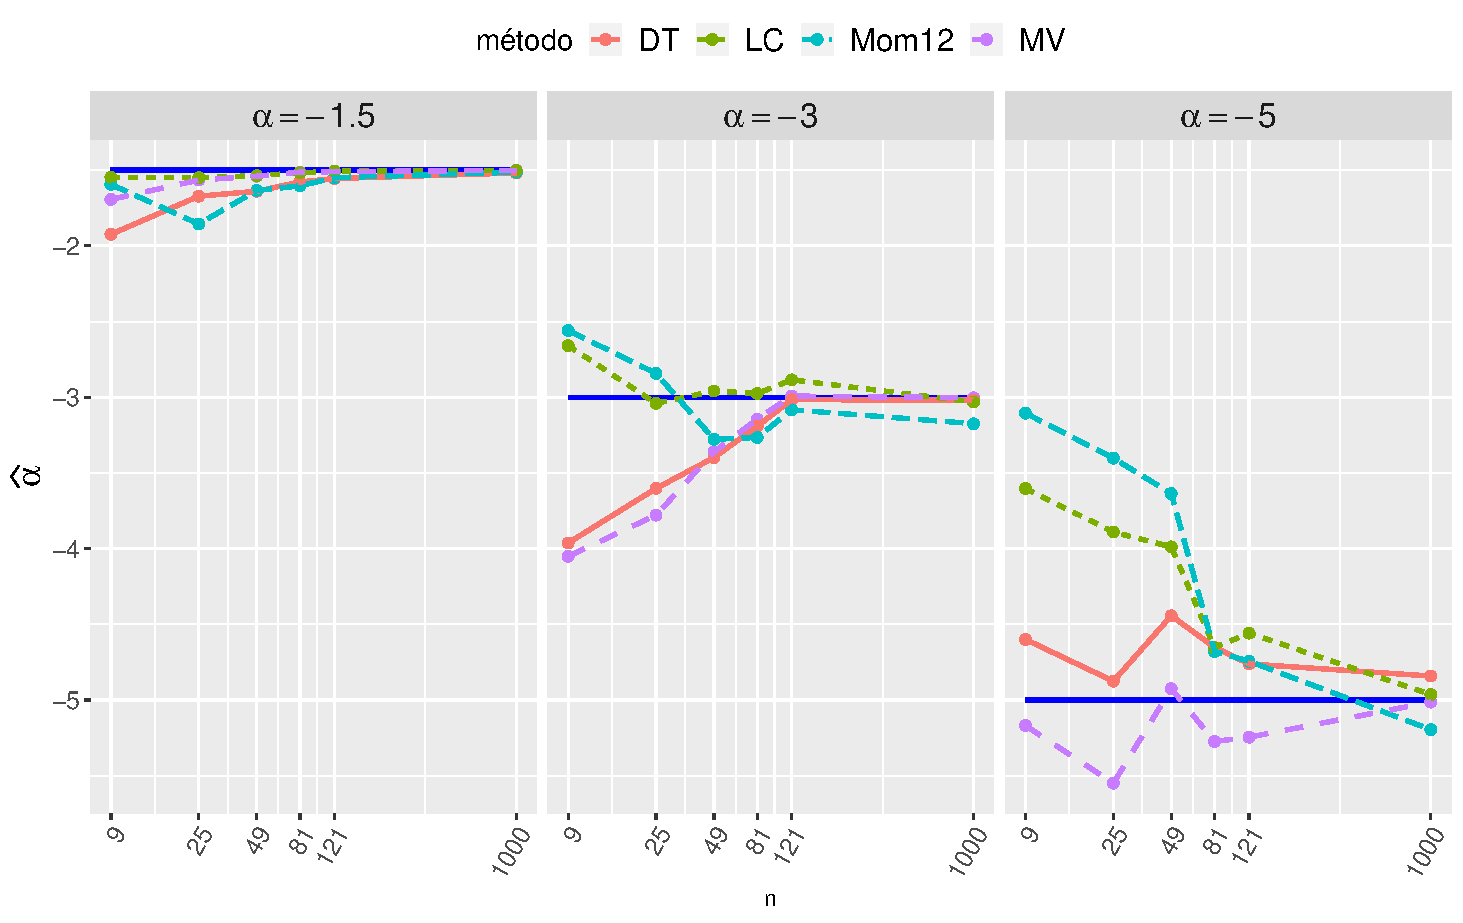
\includegraphics[width=.47\linewidth]{../../Figures/Tesis/Capitulo6/GraficoAlfaJstar2013_NoCont_L=3.pdf}}
%	\subfigure[\label{ECMEstimadosJSTAR2013_L=3}$\widehat{\text{ECM}}$, L=3]{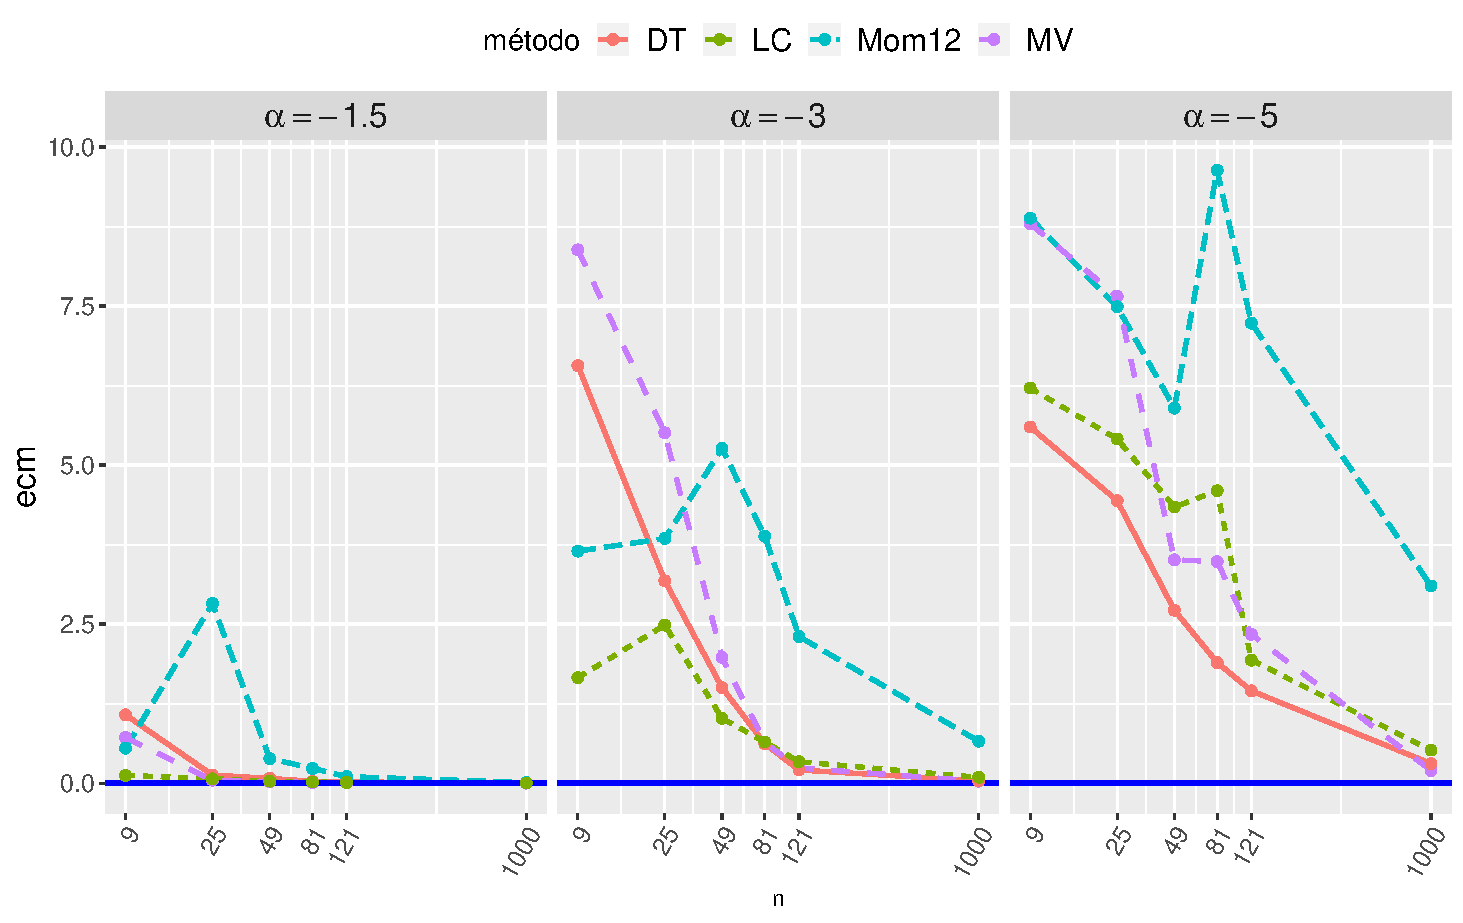
\includegraphics[width=.47\linewidth]{../../Figures/Tesis/Capitulo6/GraficoECMJstar2013_NoCont_L=3.pdf}}
	%	\subfigure[\label{AlfasEstimadosJSTAR2013_L=8}$\widehat{\alpha}$, L=8]{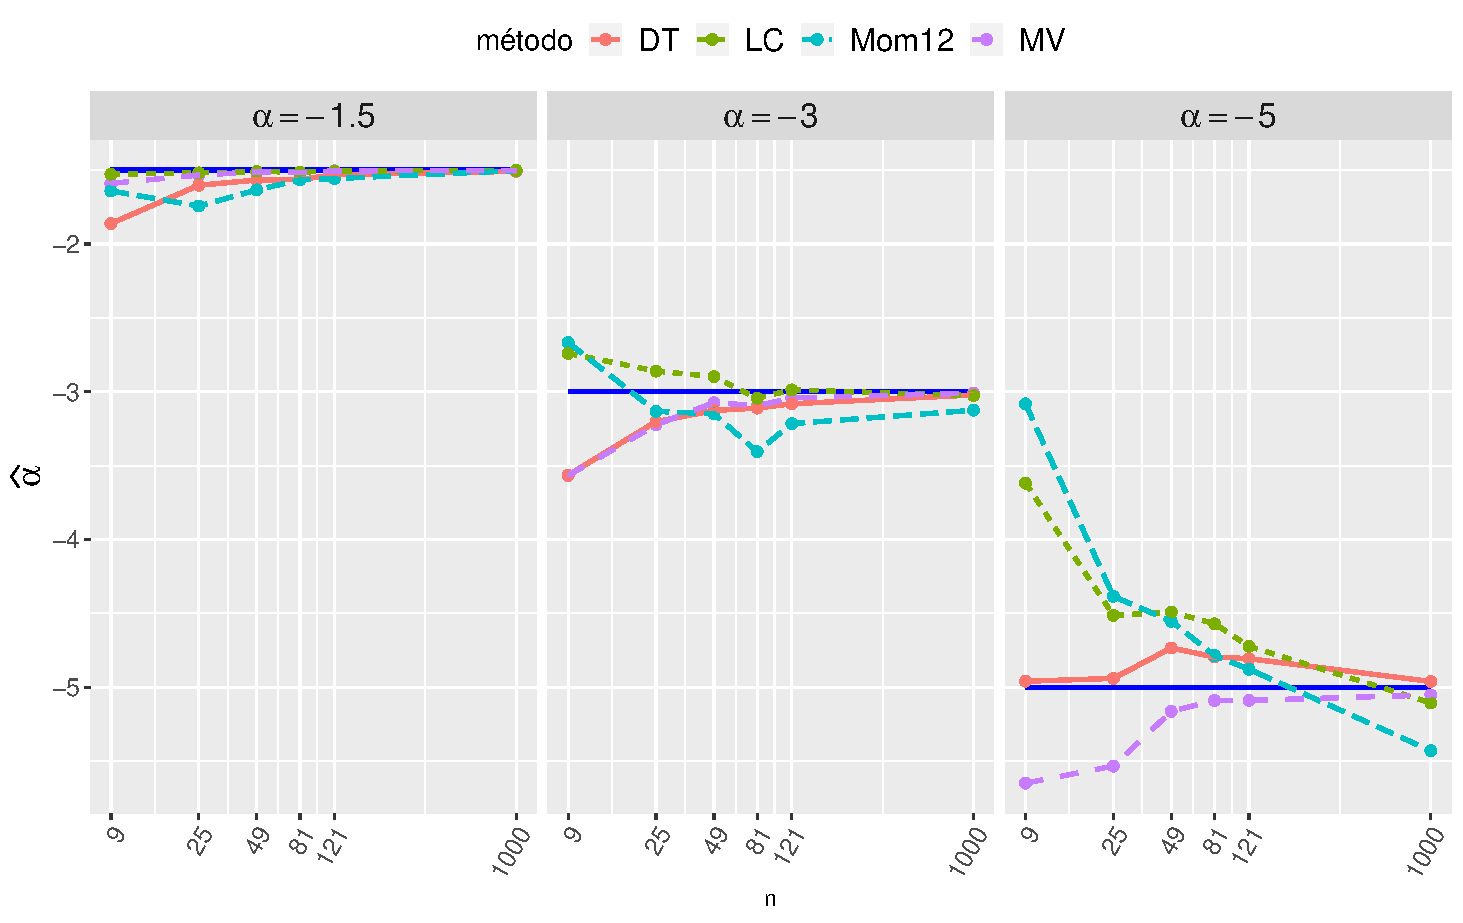
\includegraphics[width=.47\linewidth]{../../Figures/Tesis/Capitulo6/GraficoAlfaJstar2013_NoCont_L=8.pdf}}
	%	\subfigure[\label{ECMEstimadosJSTAR2013_L=8}$\widehat{\text{ECM}}$, L=8]{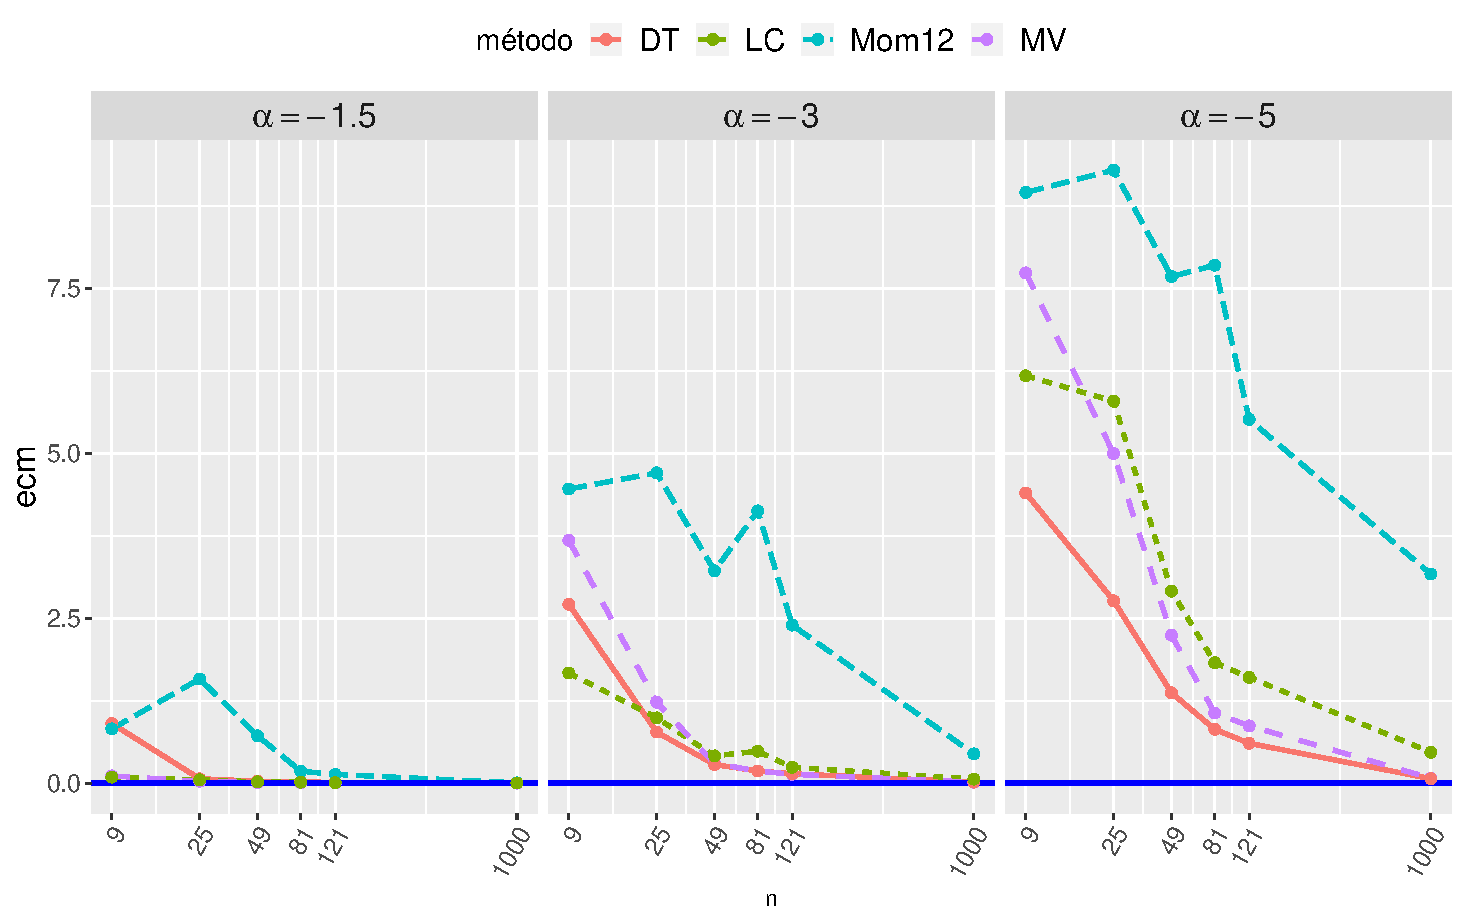
\includegraphics[width=.47\linewidth]{../../Figures/Tesis/Capitulo6/GraficoECMJstar2013_NoCont_L=8.pdf}}
	\caption{\small $\widehat{\text{Sesgo}}$ y $\widehat{\text{ECM}}$ para datos sin contaminar, $L=1$.}
\end{figure}


\begin{figure}[H]
	\centering
%	\subfigure[\label{AlfasEstimadosJSTAR2013_L=1}$\widehat{\alpha}$, L=1]{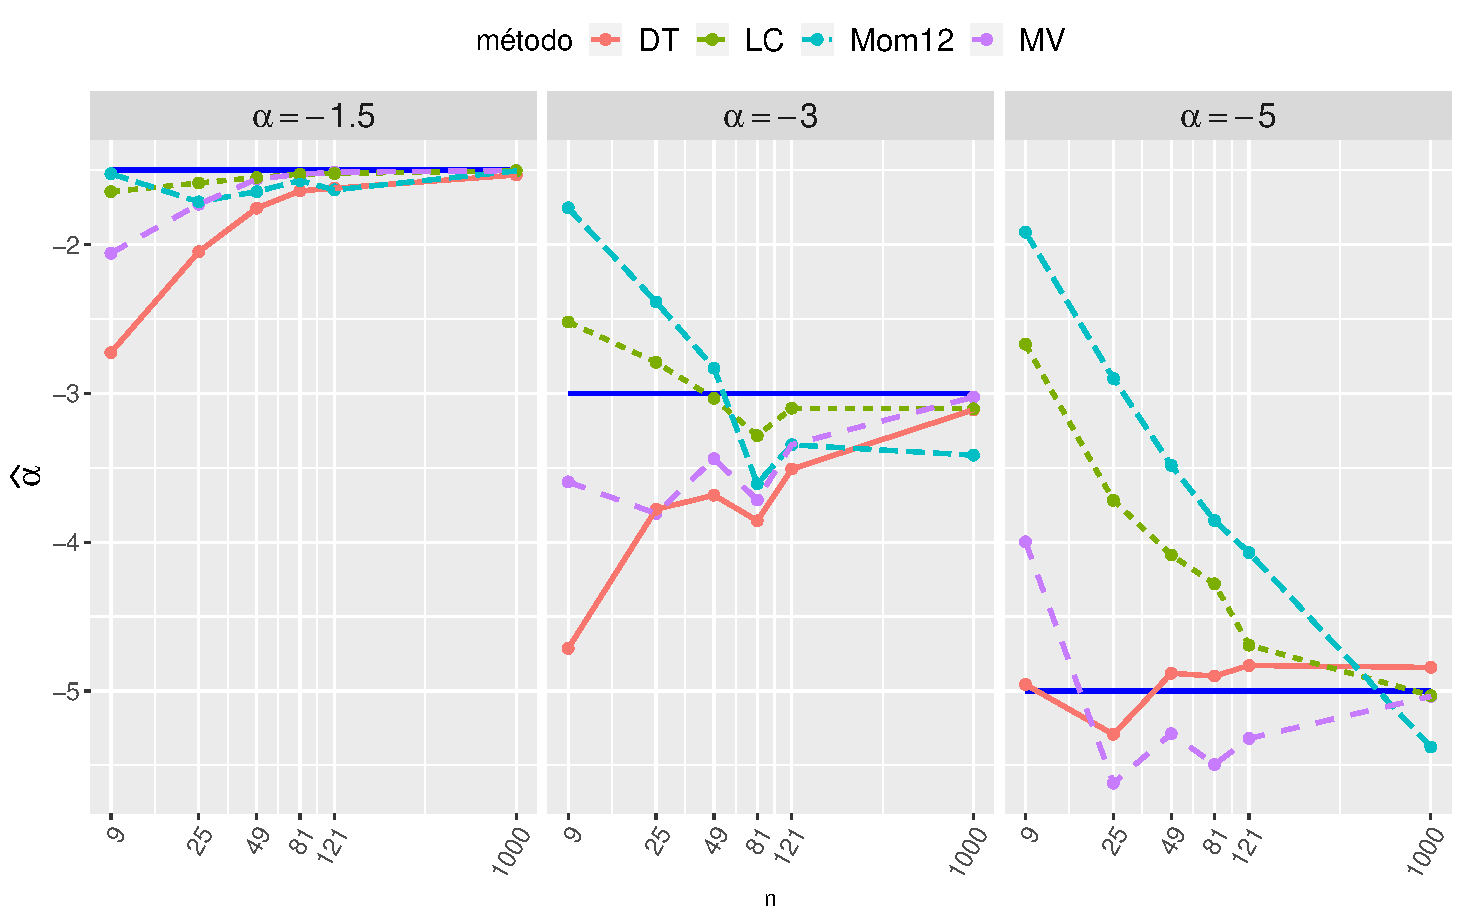
\includegraphics[width=.47\linewidth]{../../Figures/Tesis/Capitulo6/GraficoAlfaJstar2013_NoCont_L=1.pdf}}
%	\subfigure[\label{ECMEstimadosJSTAR2013_L=1}$\widehat{\text{ECM}}$, L=1]{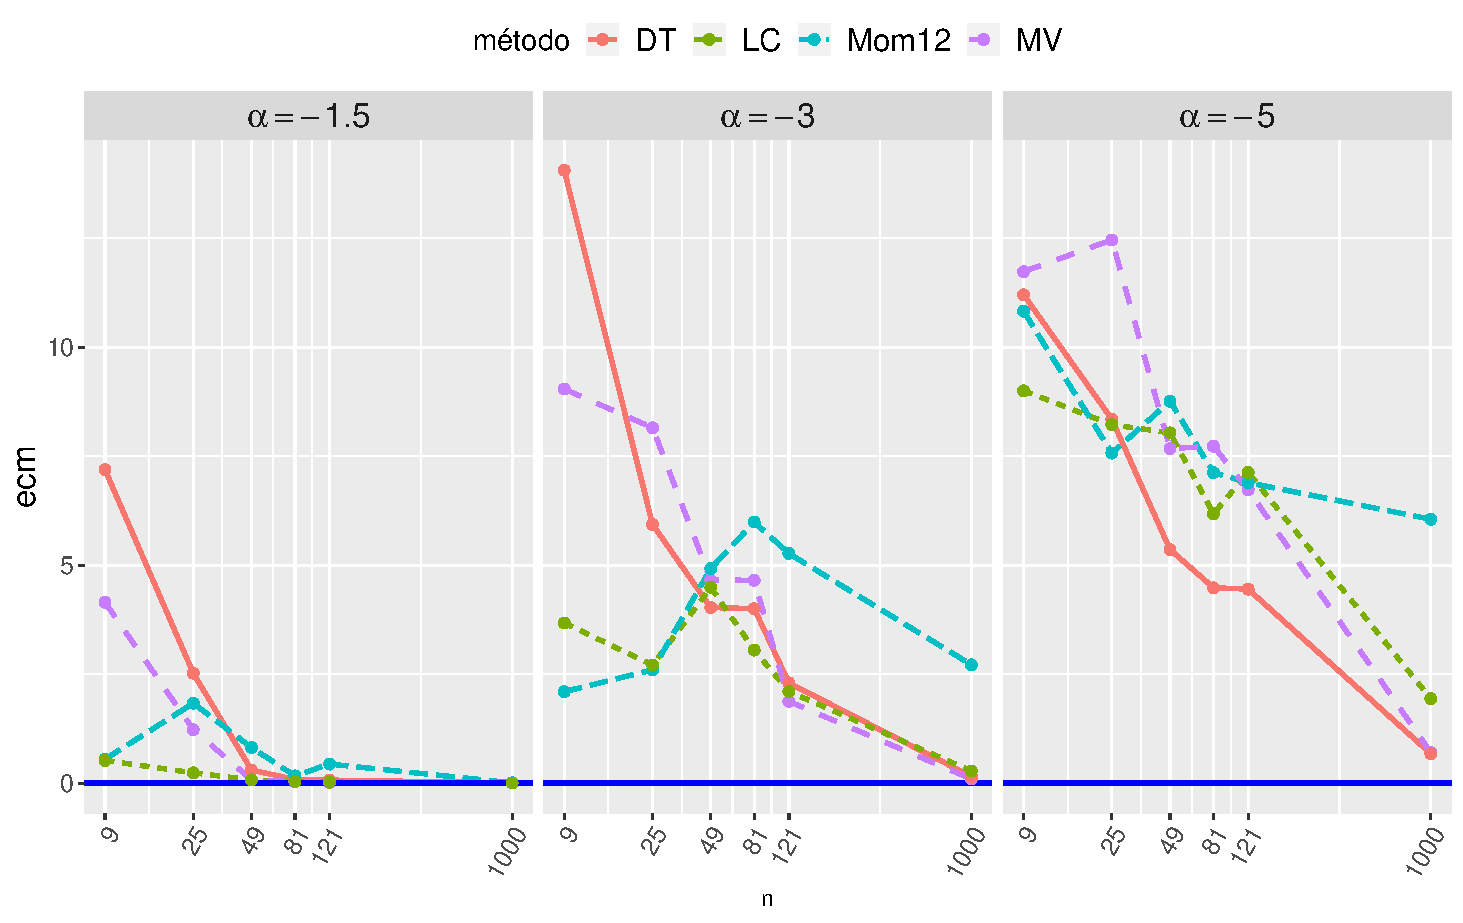
\includegraphics[width=.47\linewidth]{../../Figures/Tesis/Capitulo6/GraficoECMJstar2013_NoCont_L=1.pdf}}
	\subfigure[\label{AlfasEstimadosJSTAR2013_L=3}$\widehat{\text{Sesgo}}$]{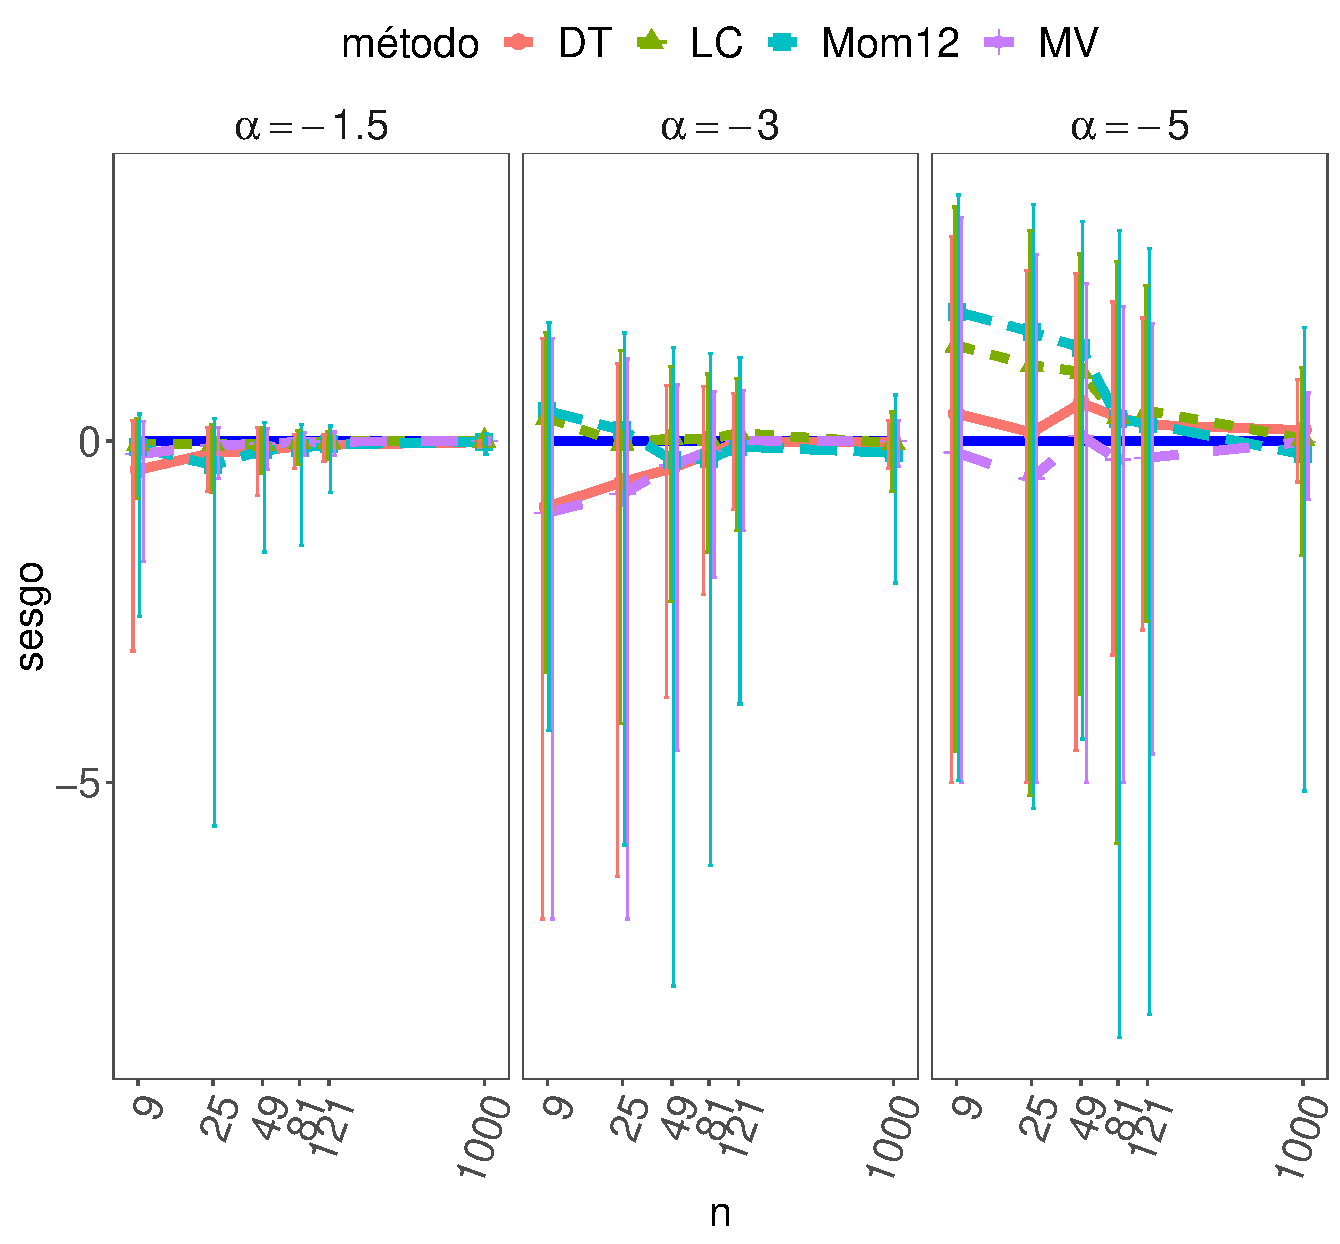
\includegraphics[width=.47\linewidth]{../../Figures/Tesis/Capitulo6/GraficoSESGOJstar2013BarrasError_NoCont_L=3ypercentil.pdf}}
	\subfigure[\label{ECMEstimadosJSTAR2013_L=3}$\widehat{\text{ECM}}$]{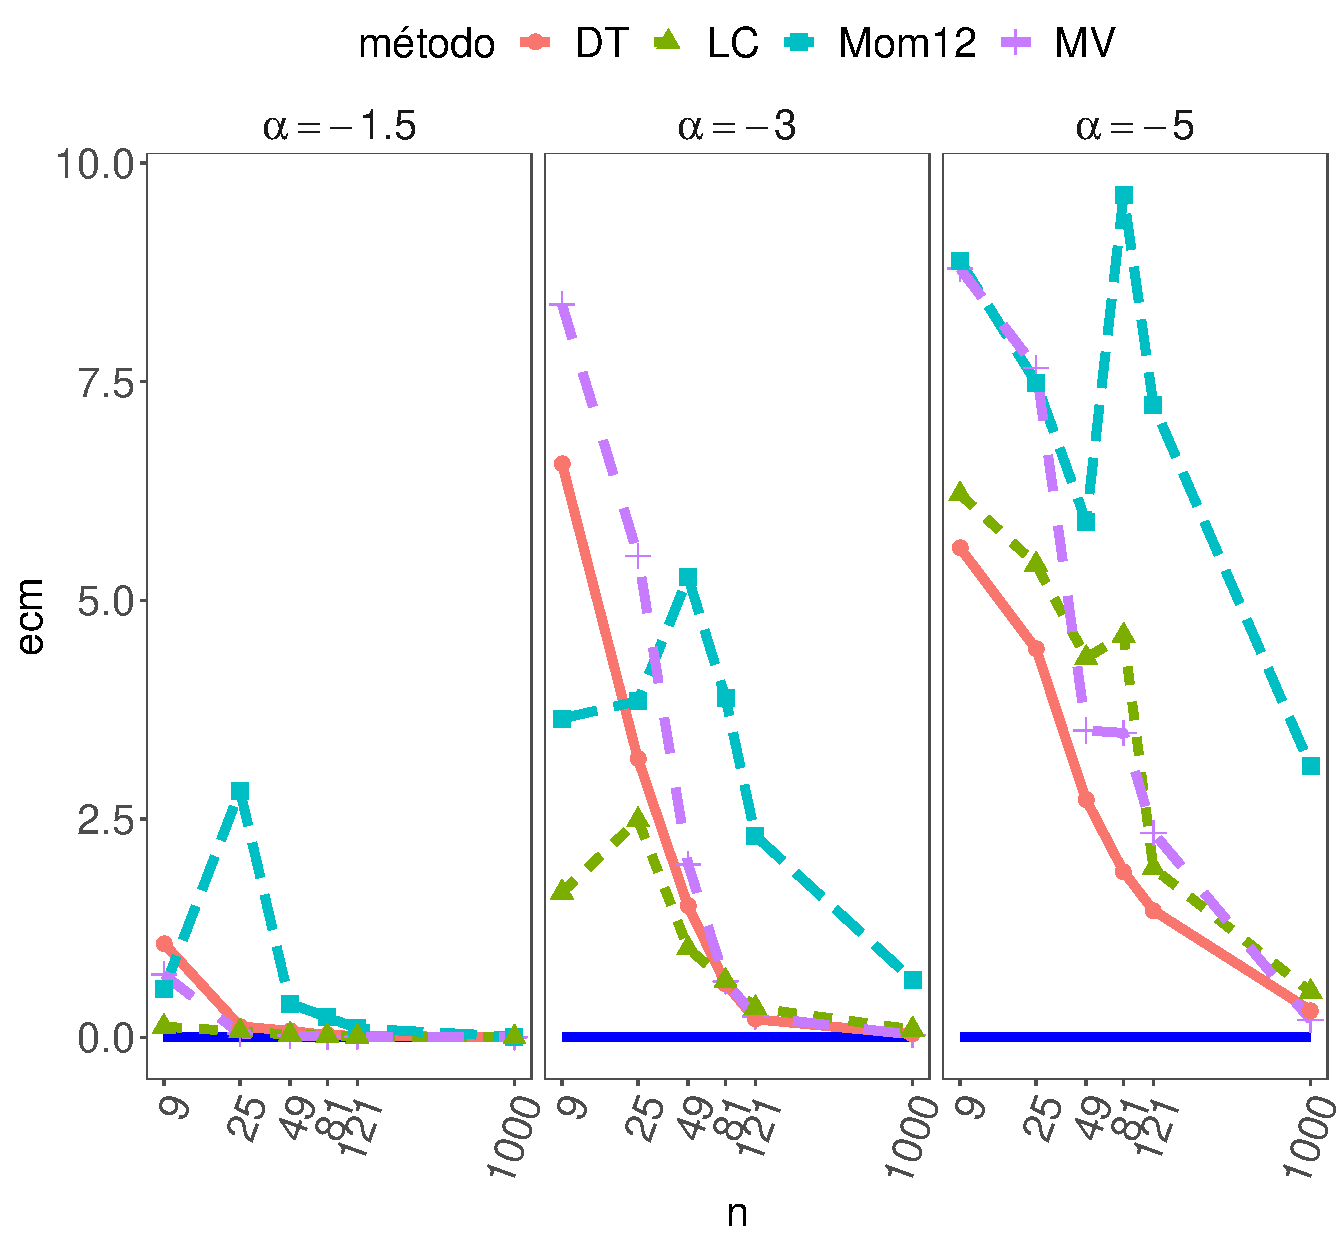
\includegraphics[width=.47\linewidth]{../../Figures/Tesis/Capitulo6/GraficoECMJstar2013BarrasError_NoCont_L=3ypercentil.pdf}}
%	\subfigure[\label{AlfasEstimadosJSTAR2013_L=8}$\widehat{\alpha}$, L=8]{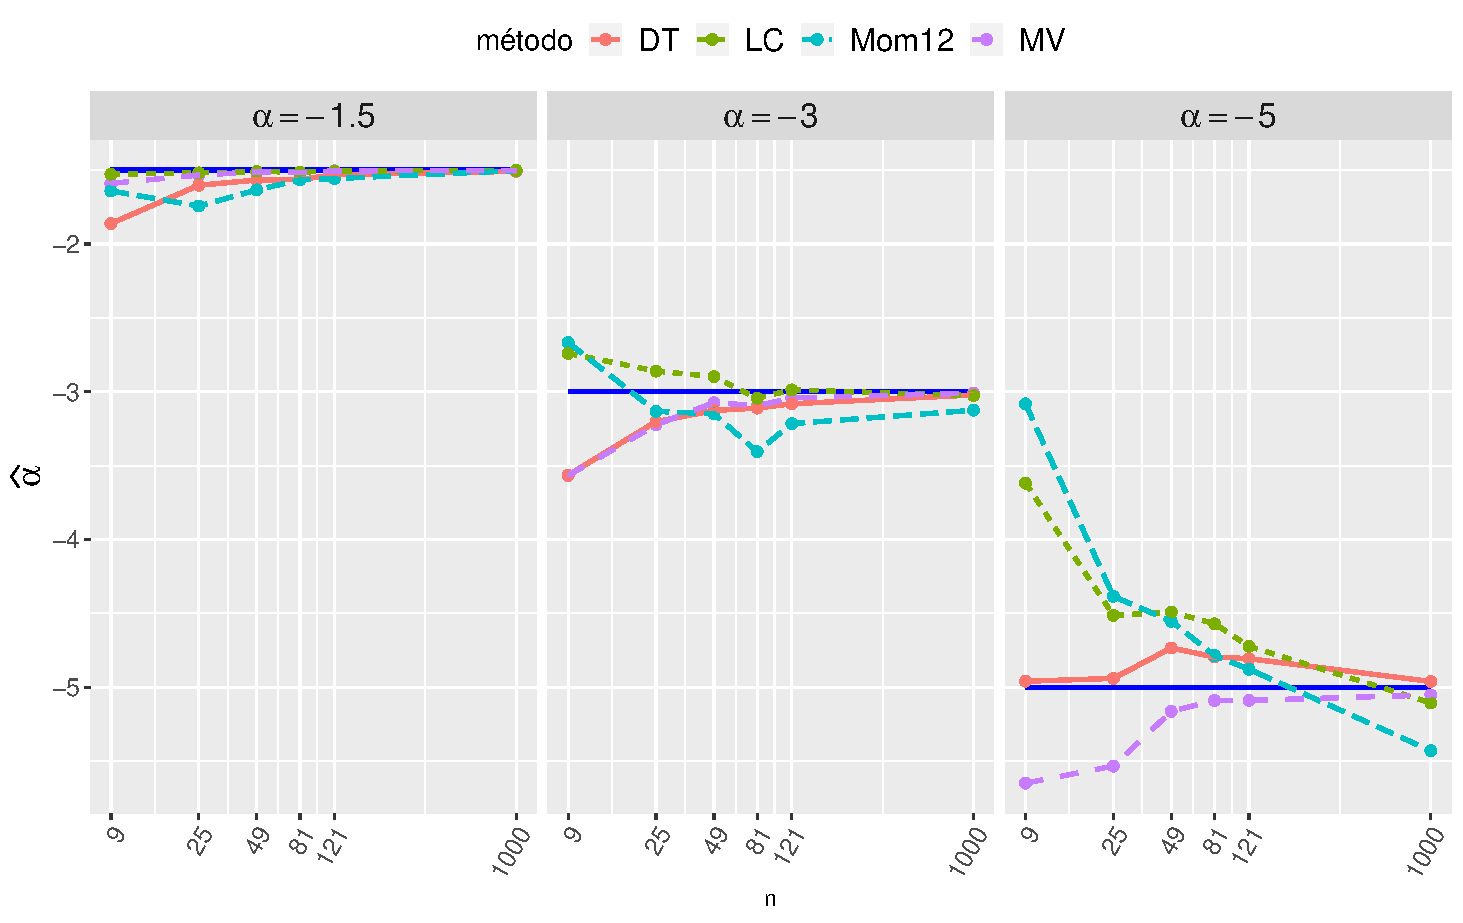
\includegraphics[width=.47\linewidth]{../../Figures/Tesis/Capitulo6/GraficoAlfaJstar2013_NoCont_L=8.pdf}}
%	\subfigure[\label{ECMEstimadosJSTAR2013_L=8}$\widehat{\text{ECM}}$, L=8]{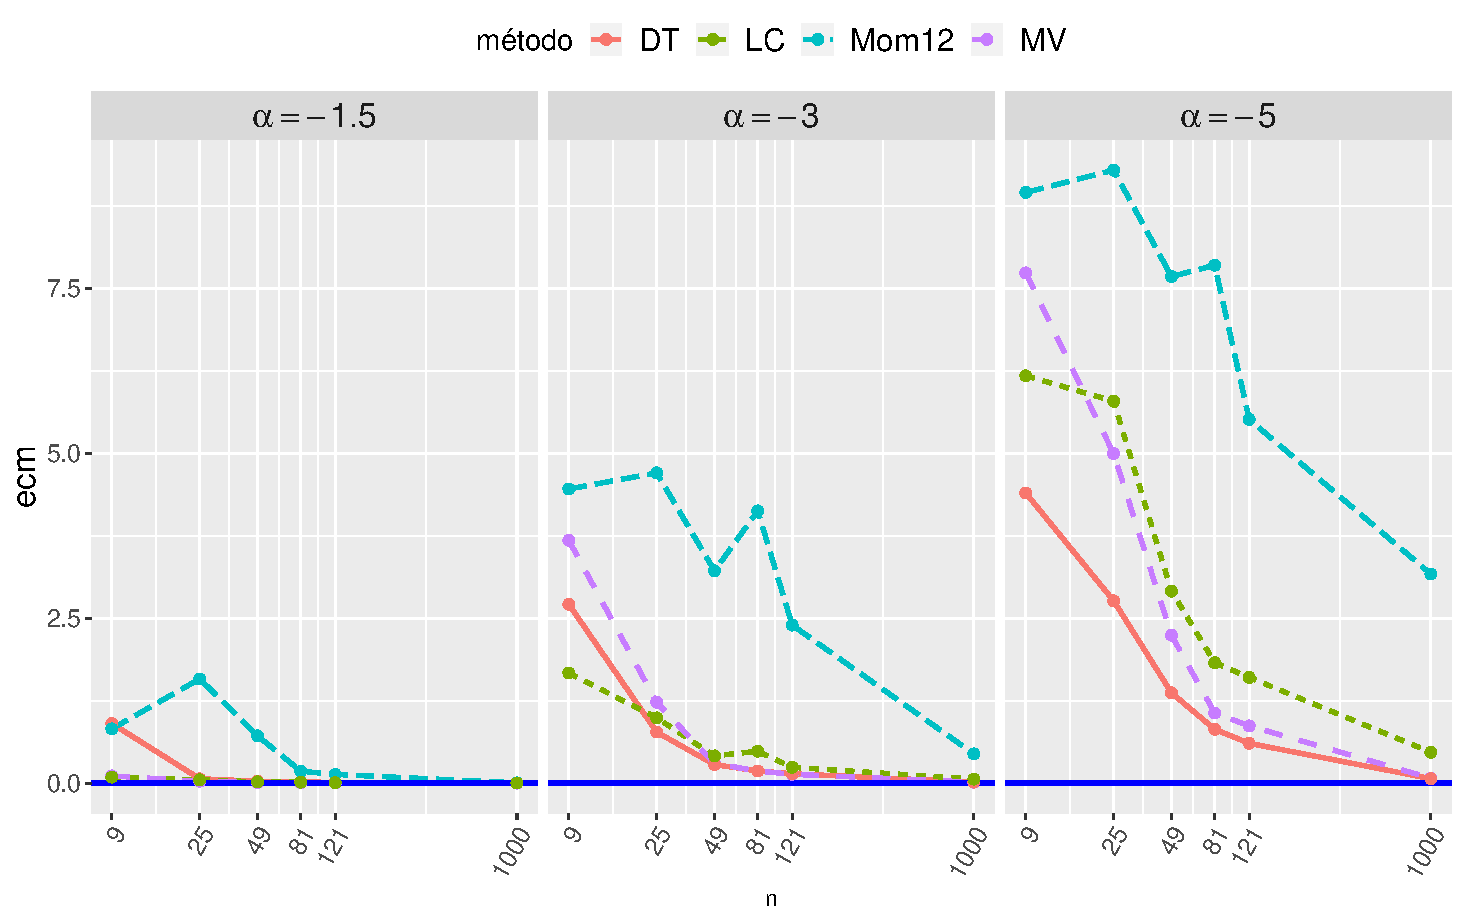
\includegraphics[width=.47\linewidth]{../../Figures/Tesis/Capitulo6/GraficoECMJstar2013_NoCont_L=8.pdf}}
	\caption{\small $\widehat{\text{Sesgo}}$ y $\widehat{\text{ECM}}$ para datos sin contaminar, $L=3$.}
\end{figure}

\begin{figure}[H]
	\centering
%	\subfigure[\label{AlfasEstimadosJSTAR2013_L=1}$\widehat{\alpha}$, L=1]{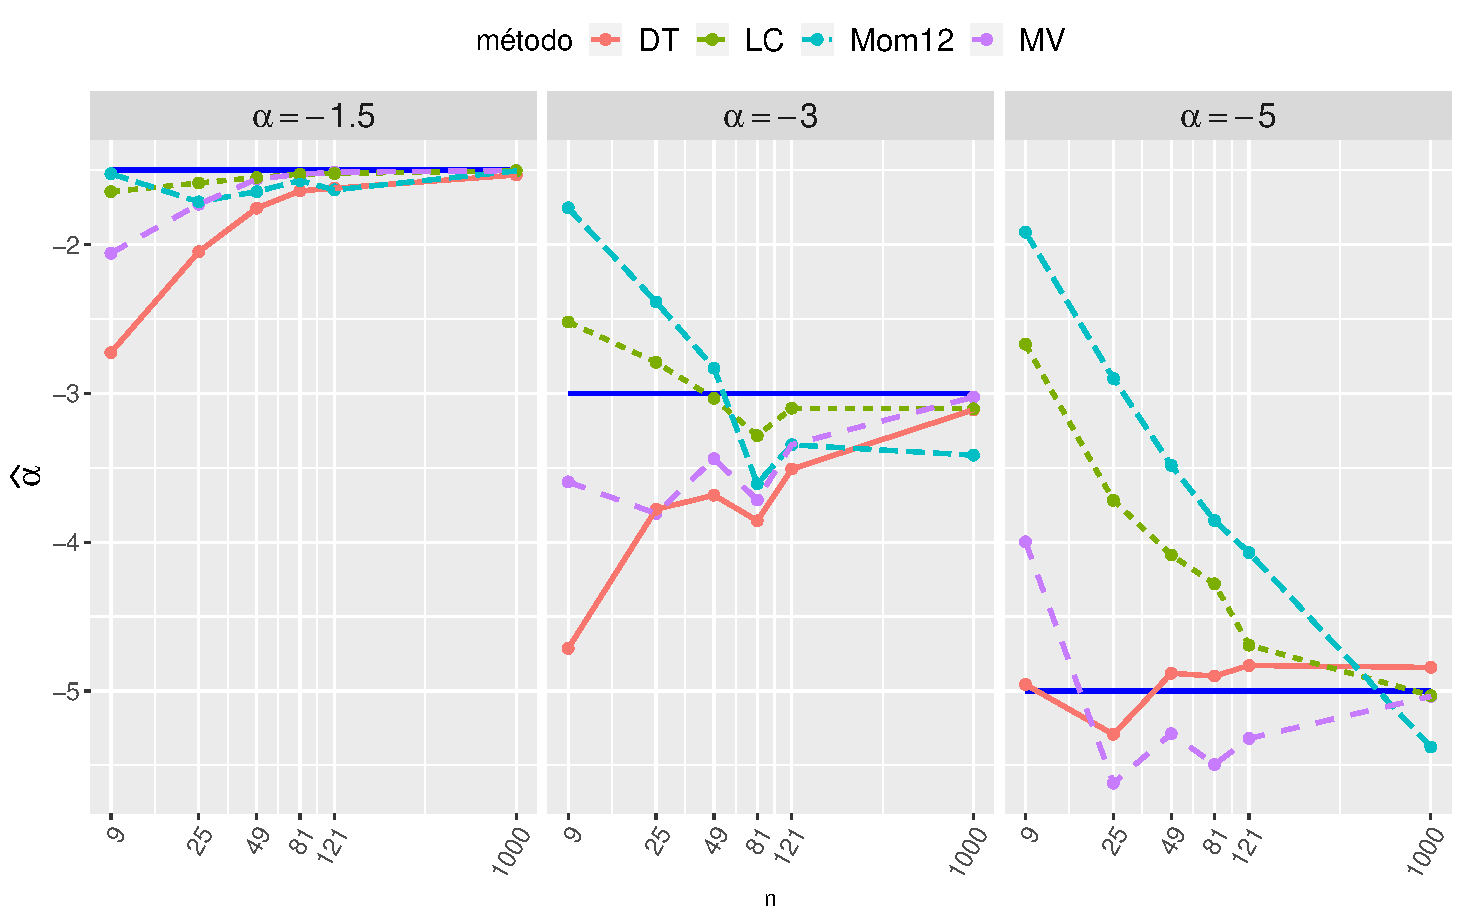
\includegraphics[width=.47\linewidth]{../../Figures/Tesis/Capitulo6/GraficoAlfaJstar2013_NoCont_L=1.pdf}}
%	\subfigure[\label{ECMEstimadosJSTAR2013_L=1}$\widehat{\text{ECM}}$, L=1]{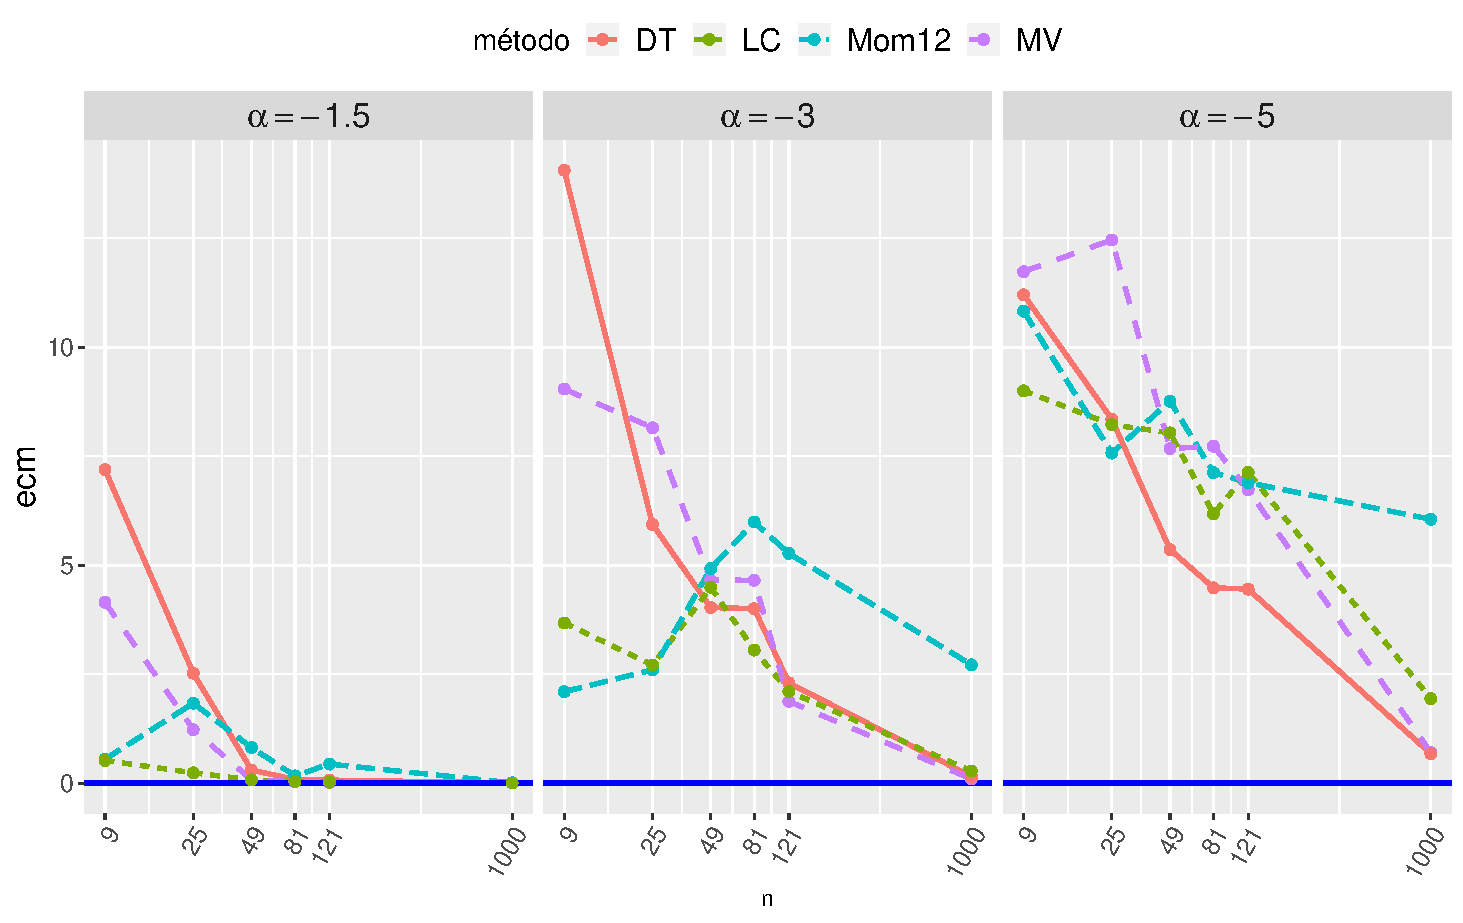
\includegraphics[width=.47\linewidth]{../../Figures/Tesis/Capitulo6/GraficoECMJstar2013_NoCont_L=1.pdf}}
%	\subfigure[\label{AlfasEstimadosJSTAR2013_L=3}$\widehat{\alpha}$, L=3]{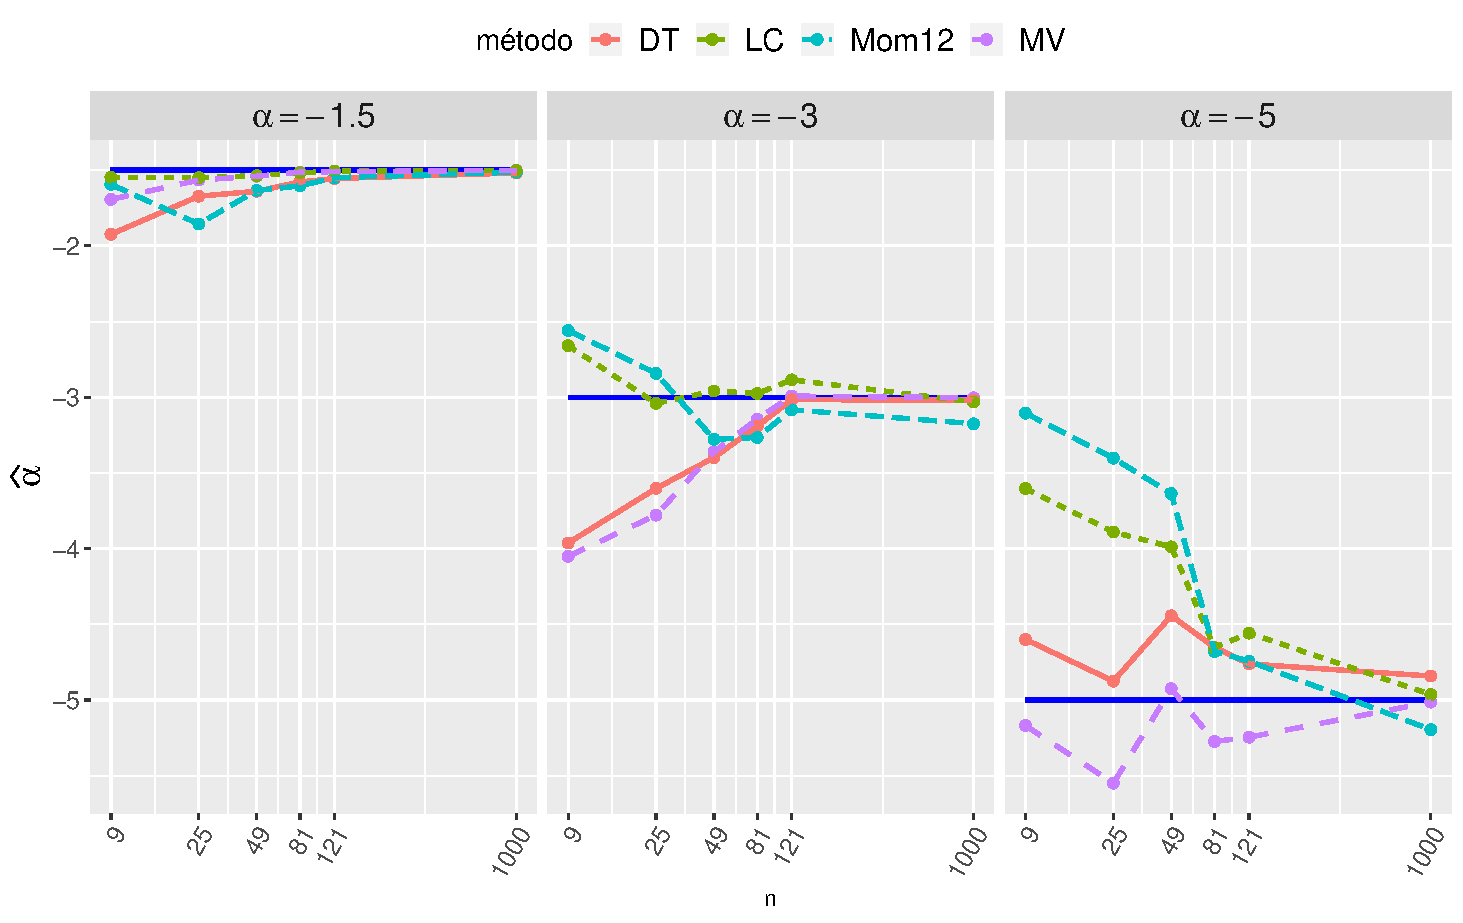
\includegraphics[width=.47\linewidth]{../../Figures/Tesis/Capitulo6/GraficoAlfaJstar2013_NoCont_L=3.pdf}}
%	\subfigure[\label{ECMEstimadosJSTAR2013_L=3}$\widehat{\text{ECM}}$, L=3]{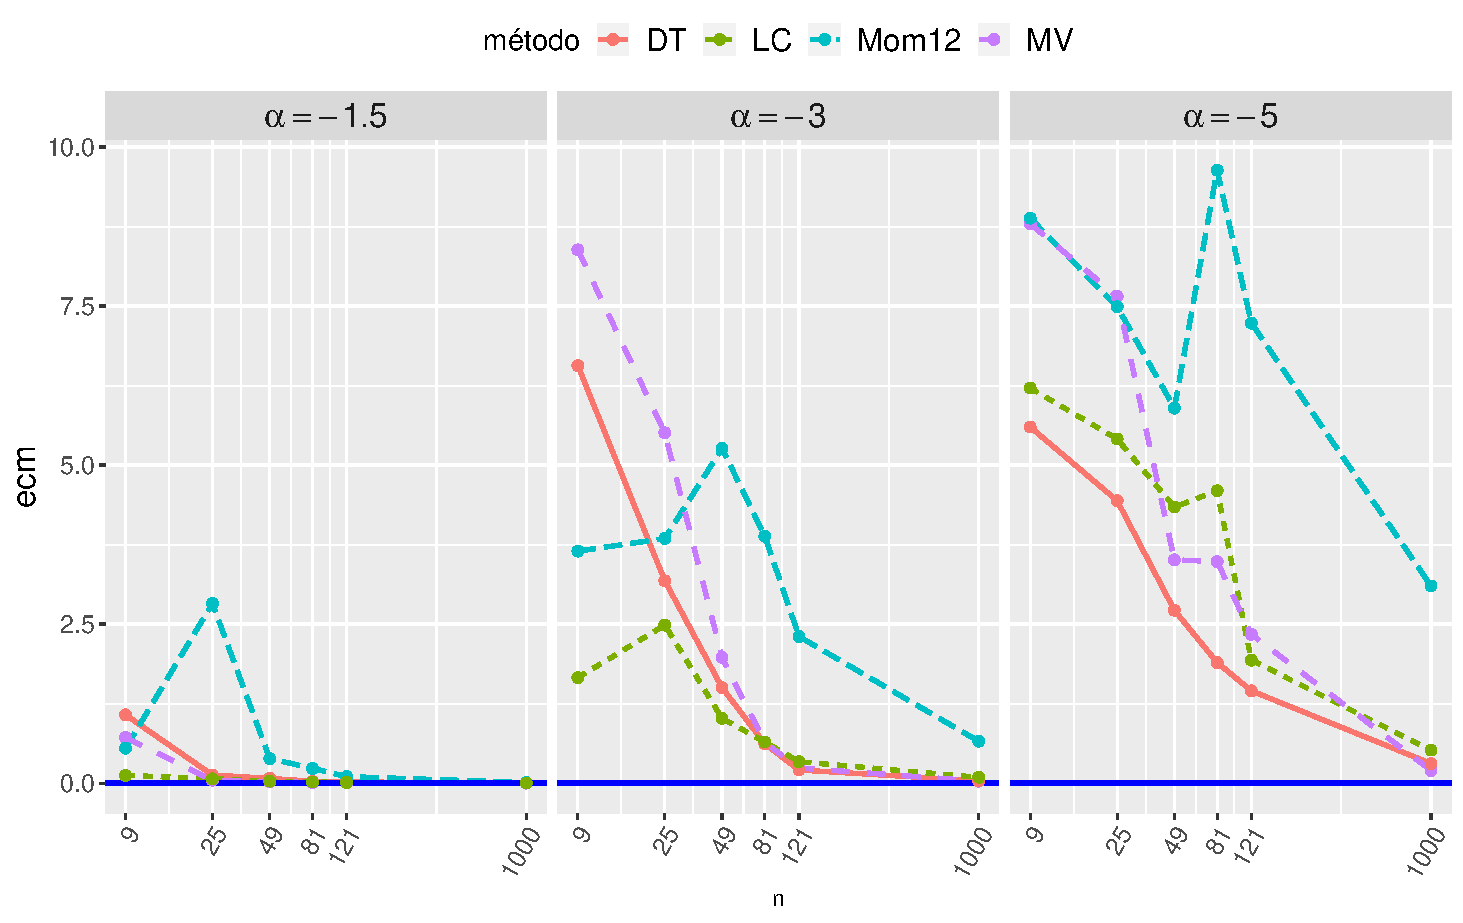
\includegraphics[width=.47\linewidth]{../../Figures/Tesis/Capitulo6/GraficoECMJstar2013_NoCont_L=3.pdf}}
	\subfigure[\label{AlfasEstimadosJSTAR2013_L=8}$\widehat{\text{Sesgo}}$]{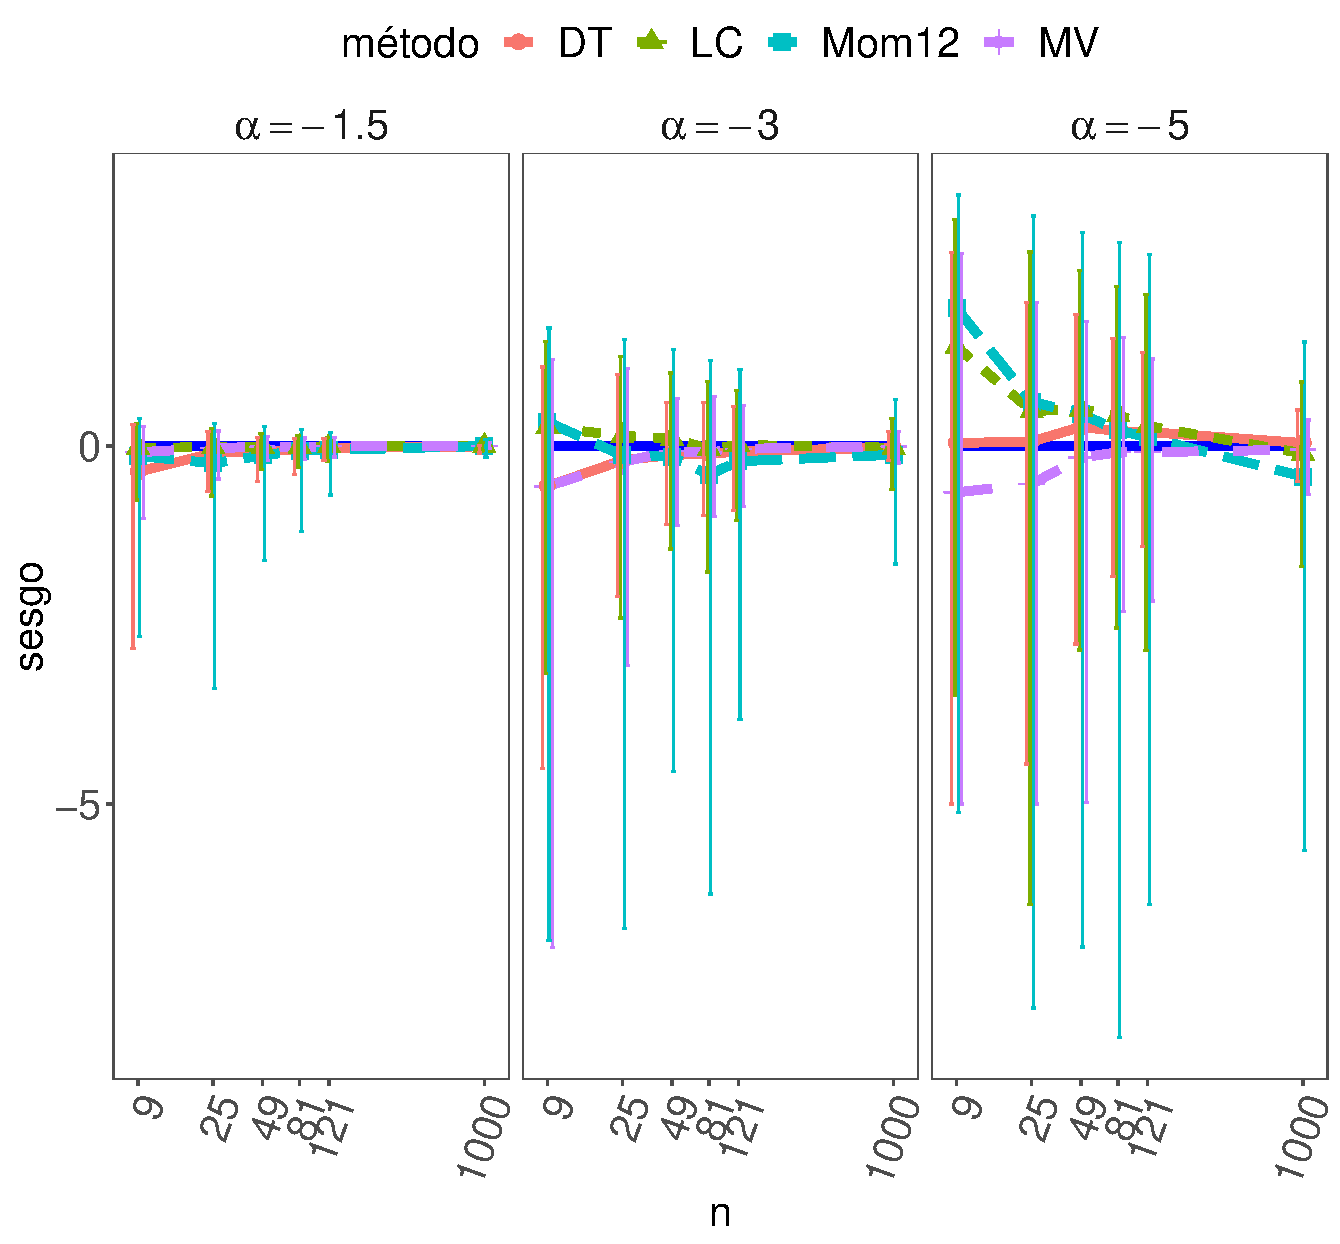
\includegraphics[width=.47\linewidth]{../../Figures/Tesis/Capitulo6/GraficoSESGOJstar2013BarrasError_NoCont_L=8ypercentil.pdf}}
	\subfigure[\label{ECMEstimadosJSTAR2013_L=8}$\widehat{\text{ECM}}$]{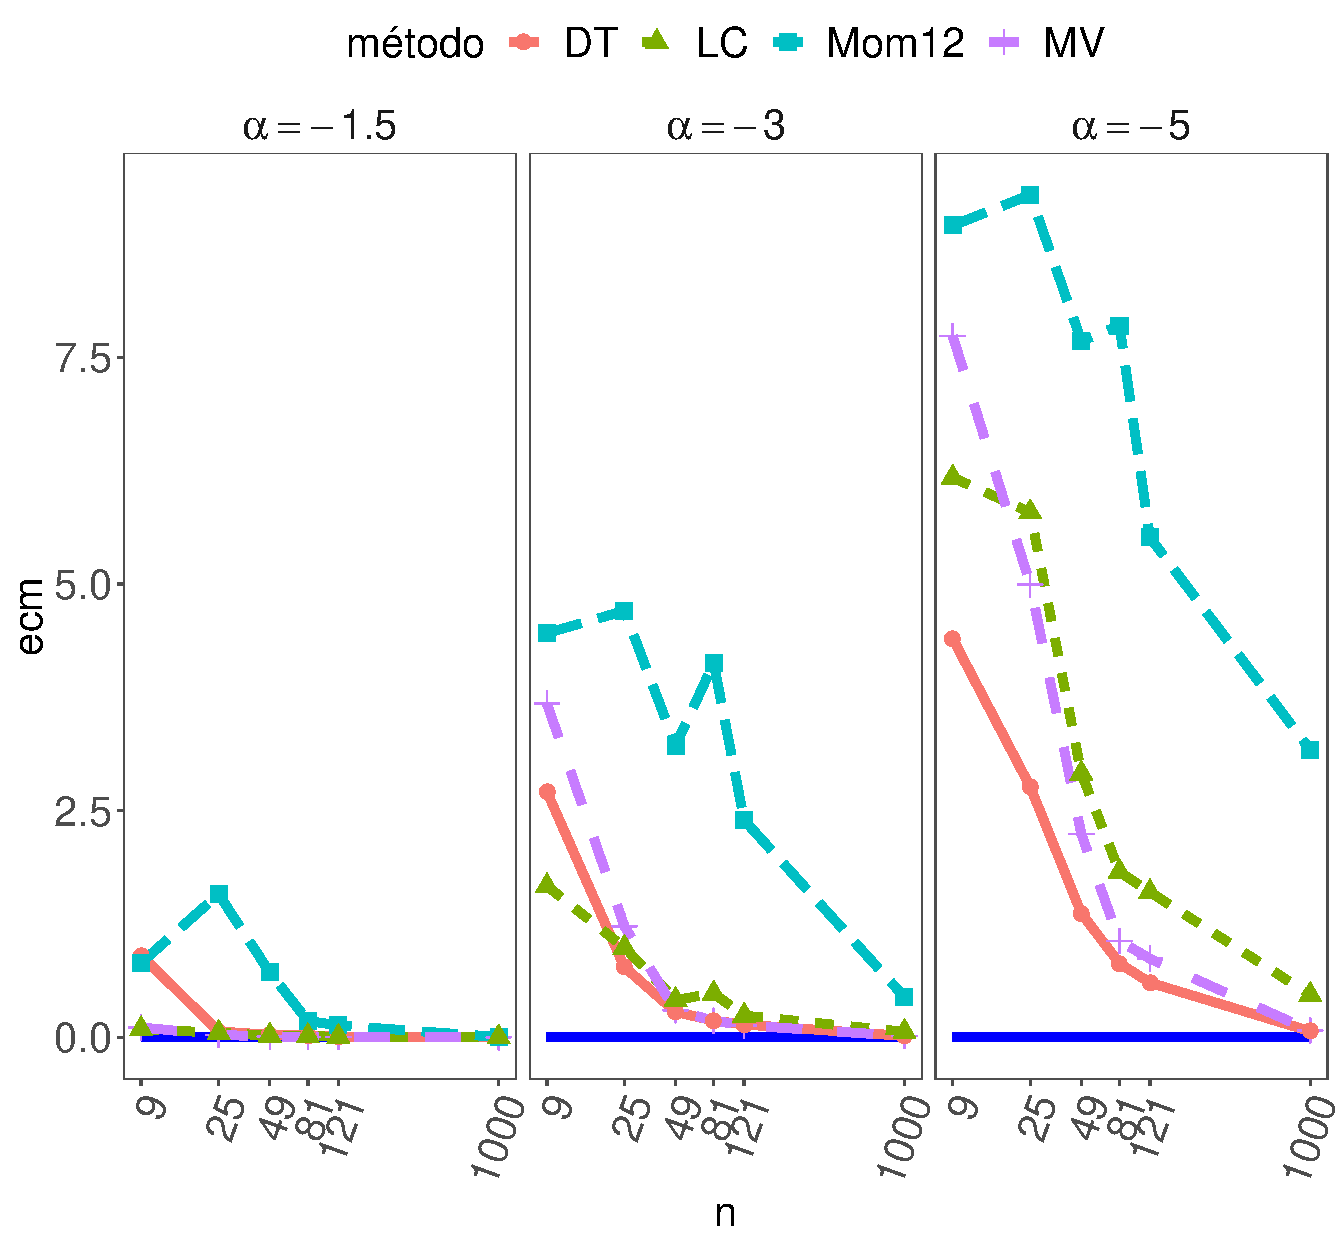
\includegraphics[width=.47\linewidth]{../../Figures/Tesis/Capitulo6/GraficoECMJstar2013BarrasError_NoCont_L=8ypercentil.pdf}}
	\caption{\small $\widehat{\text{Sesgo}}$ y $\widehat{\text{ECM}}$ para datos sin contaminar, $L=8$.}
\end{figure}

%%%%%%%%%%%%%%%%%%%%%%%%%%%%%%%%%%%%%%%%%%%%%%%%%%%%%%%%%% TIEMPO
Se calculó el tiempo medio de procesamiento, medido en segundos, para cada método y cada caso estudiado. Como  ejemplo se presenta, en la tabla~\ref{tablaDeTiemposmedios}, el tiempo medio para $L=1$ y $n=81$. Se puede observar que nuestra propuesta tiene un mayor costo computacional debido a la integración numérica presente en la definición del estimador. Los otros casos son consistentes con los datos de esta tabla. 
La plataforma informática que se utilizó para realizar los procesos fue Intel(R) Core i7, con 8GB de memoria y 64 bits Windows 7. 

\begin{table}[htb]
	\centering
	\begin{tabular}{cccc}
		\toprule
		MV& DT& Mom$\frac{1}{2}$ & LC \\
		\midrule
		$0.003$& $2.223$ & $0.0001$ &$0.003$ \\
		\bottomrule
	\end{tabular}
\caption{\label{tablaDeTiemposmedios}\small Tiempos medios para datos simulados sin contaminación, $L=1$, $n=81$. }
\end{table}

%%%%%%%%%%%%%%%%%%%%%%%%%%%%%%%%%%%%%%%%%%%%%%%%%%%%%%%%%% ROBUSTEZ
\subsection{Evaluando Robustez}

Es muy importante contar con estimadores que sean resistentes a la presencia de datos contaminados, es decir, que sean capaces de producir buenas estimaciones incluso cuando una proporción de los datos no proviene del modelo supuesto como verdadero. Esta situación es de particular importancia en el caso de muestras de pequeño tamaño, por ejemplo, cuando se utilizan filtros que emplean estimadores basados, por lo general, en pequeñas muestras ya que recorren la imagen a través de ventanas deslizantes de tamaño $3 \times 3$, $5 \times 5$ o, por ejemplo, $7 \times 7$. Estas muestras pueden tener datos de zonas con diferentes grado de textura, por ejemplo, en el borde entre diferentes regiones. Esta capacidad de producir buenas estimaciones cuando las observaciones no provienen exactamente del modelo asumido se llama Robustez.

Una de las fuentes de contaminación en las imágenes SAR es el fenómeno de Double Bounce, donde algunos píxeles tienen un alto valor de retorno.  La presencia de tales valores atípicos puede provocar grandes errores en la estimación. La descripción de este fenómeno se hizo en la sección~\ref{SecDobleBounce}.

Con el fin de evaluar la robustez de los estimadores, proponemos tres escenarios capaces de describir los desvíos del modelo teórico. Para cada uno de estos escenarios generamos muestras contaminadas donde $0<\epsilon \ll 1$ es la proporción de contaminación. 
Sea  $B$ una variable aleatoria Bernoulli con probabilidad $\epsilon$ de ocurrencia de la contaminación. Sea $C \in \mathbb R_+$ un valor grande. Entonces
\begin{itemize}
	\item \label{ContCaso1}Caso~1:
	Sean $W$ y $U$ variables aleatorias tales que $W \sim \mathcal{G}_I^0(\alpha_1,\gamma_1^*,L)$, y $U \sim \mathcal{G}_I^0(\alpha_2,\gamma_2^*,L) $. Definimos $Z=BU+(1-B)W$, entonces generamos $\{z_1,\dots,z_n\}$ variables aleatorias independientes, idénticamente distribuidas con función de distribución acumulada dada por:
	$$
	(1-\epsilon) \mathcal{F}_{\mathcal{G}_I^0(\alpha_1,\gamma_1^*,L)}(z)+\epsilon\mathcal{F}_{\mathcal{G}_I^0(\alpha_2,\gamma_2^*,L)}(z),
	$$
	donde $\mathcal{F}_{\mathcal{G}_I^0(\alpha,\gamma,L)}$ es la función de distribución acumulada bajo el modelo $\mathcal{G}_I^0(\alpha,\gamma,L)$.
	%
	\item \label{Caso2}Caso~2: Consideramos $W \sim \mathcal{G}_I^0(\alpha_1,\gamma_1^*,L)$ y el retorno definido como $Z=BC+(1-B)W$.
	\item \label{Caso3}Caso~3:
	Consideramos $W \sim \mathcal{G}_I^0(\alpha,\gamma^*,L)$ y $U\sim \mathcal{G}_I^0(\alpha,10^k\gamma^*,L) $ con $k \in \mathbb{N}$. 
	El retorno $Z$ se define como el Caso 1 y la función de distribución acumulada está dada por: 
	$$
	(1-\epsilon) \mathcal{F}_{\mathcal{G}_I^0(\alpha,\gamma^*,L)}(z)+\epsilon\mathcal{F}_{\mathcal{G}_I^0(\alpha,10^k\gamma^*,L)}(z).
	$$
\end{itemize}

Todos estos modelos consideran desvíos de la hipótesis del modelo teórico. El primer tipo de contaminación asume que, con probabilidad $\epsilon$, los datos pueden provenir de una distribución perteneciente a la familia de distribuciones $\mathcal{G}_I^0$ pero con otros parámetros. El segundo caso contamina, con probabilidad $\epsilon$, con una constante con valor grande y fijo, digamos $C=100$. El tercer tipo de contaminación es un caso particular del primero, donde la contaminación asume que los datos provienen de una distribución cuyo factor de escala es $k$ órdenes de magnitud mayor que el factor de escala correspondiente al modelo teórico. Analizamos estos tres casos de la contaminación en la evaluación de cada estimador.

%%%%%%%%%%%%%%%%%%%%%%%%%%%%%%%%%%%%%%%%%%%%%%%%%%%%%%%%%%%%%
%%% CASE 1, alpha_2 = -15, epsilon = 0.005

Las figuras~\ref{Caso1L1},~\ref{Caso1L3} y~\ref{Caso1L8} muestran el sesgo y el ECM estimado ($\widehat{\text{ECM}}$) para el Caso $1$ de contaminación con $\alpha_2=-15$, $\epsilon=0.01$, y variando $n$ y $L$.  
Este tipo de contaminación introduce, con probabilidad $\epsilon=0.01$, observaciones casi sin textura en la muestra bajo análisis. Como se espera, la influencia de tal perturbación es más notable en aquella situaciones donde el modelo subyacente está más alejado de la contaminación. Es decir, para valores grandes de $\alpha$. Esto se ve con claridad en las figuras~\ref{ECMContJSTAR2013Caso1_L=1},\ref{ECMContJSTAR2013Caso1_L=3} y \ref{ECMContJSTAR2013Caso1_L=8} donde el $\widehat{\text{ECM}}$ de $\widehat{\alpha}_{\text{\tiny{MV}}}$, $\widehat\alpha_{\text{\tiny{Mom12}}}$ y $\widehat\alpha_{\text{\tiny{LC}}}$ son mayores que el error cuadrático medio de $\widehat\alpha_{\text{\tiny{DT}}}$ para $L=3,8$, pero esto no es tan claro para el caso de $L=1$. Lo que si se puede decir que $\widehat\alpha_{\text{\tiny{DT}}}$ es competitivo respecto de los otros estimadores para $\alpha=-3,-5$.

\begin{figure}[htb]
	\subfigure[\label{AlfasContJSTAR2013Caso1_L=1}$\widehat{\text{Sesgo}}$]{\includegraphics[width=.48\linewidth]{../../Figures/Tesis/Capitulo6/GraficoSesgoJstar2013_Cont_L=1Caso1BarrasErrorypercentil.pdf}}
	\subfigure[\label{ECMContJSTAR2013Caso1_L=1}$\widehat{\text{ECM}}$]{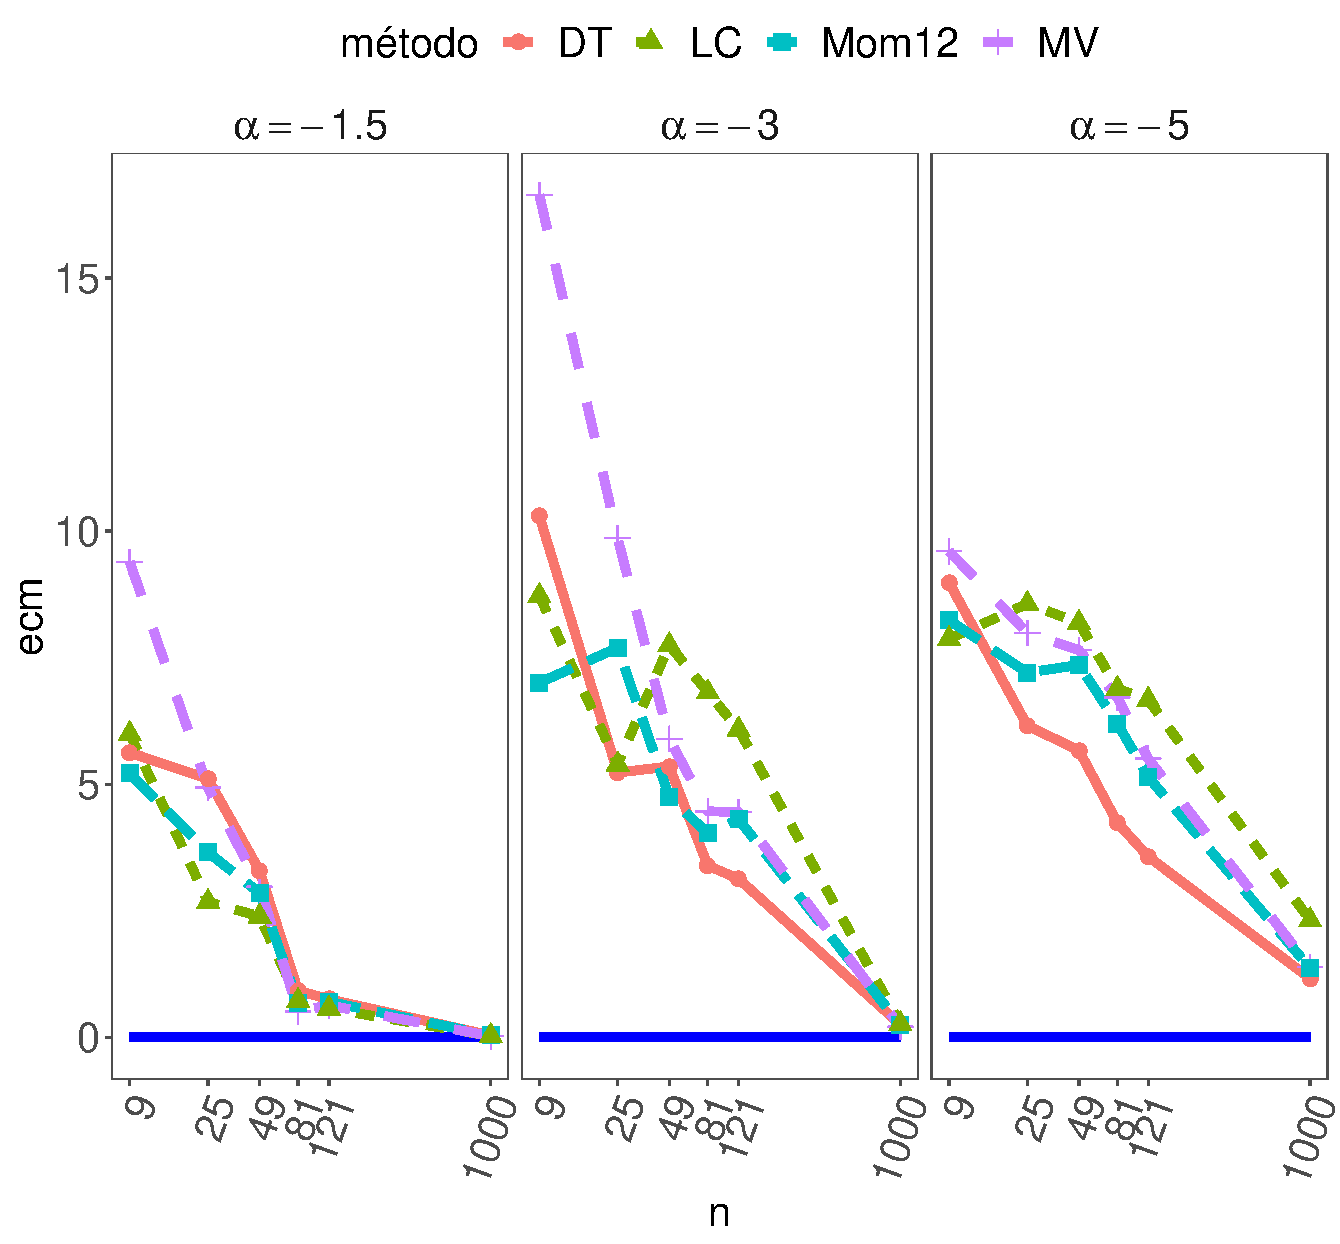
\includegraphics[width=.48\linewidth]{../../Figures/Tesis/Capitulo6/GraficoECMJstar2013_Cont_L=1Caso1BarrasErrorypercentil.pdf}}
%	\subfigure[\label{AlfasContJSTAR2013Caso1_L=3}$\widehat{\alpha}$, L=3]{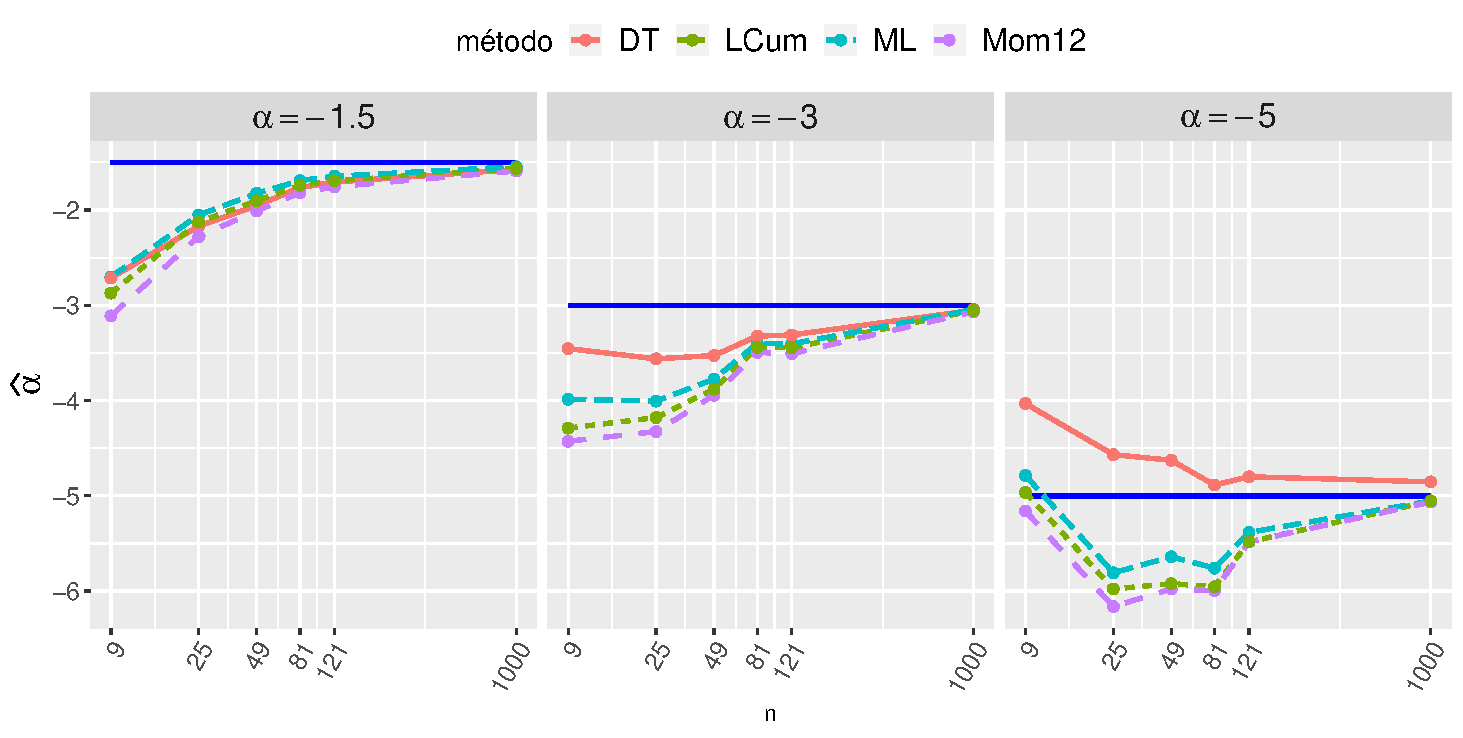
\includegraphics[width=.48\linewidth]{../../Figures/Tesis/Capitulo6/GraficoAlfaJstar2013_Cont_L=3Caso1.pdf}}
%	\subfigure[\label{ECMContJSTAR2013Caso1_L=3}$\widehat{\text{ECM}}$, L=3]{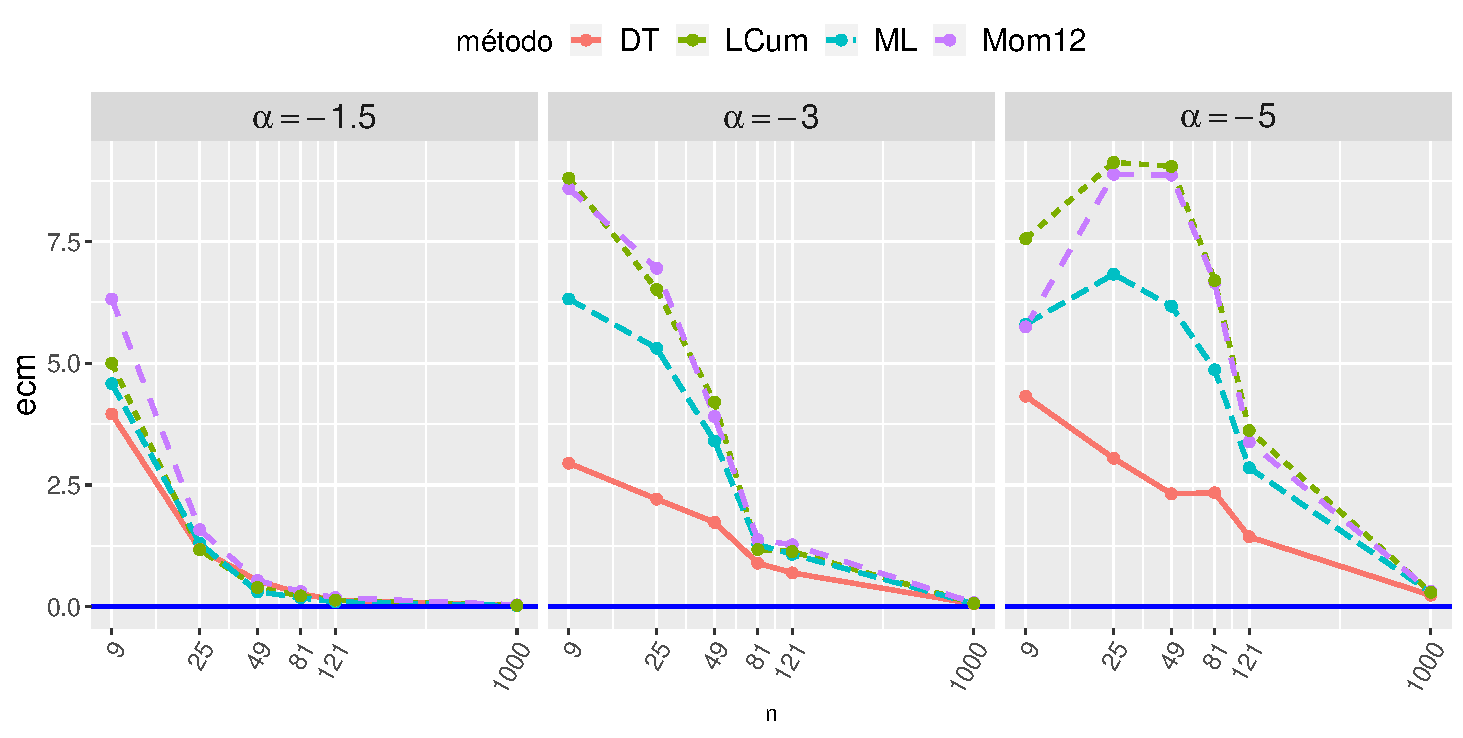
\includegraphics[width=.48\linewidth]{../../Figures/Tesis/Capitulo6/GraficoECMJstar2013_Cont_L=3Caso1.pdf}}
%	\subfigure[\label{AlfasContJSTAR2013Caso1_L=8}$\widehat{\alpha}$, L=8]{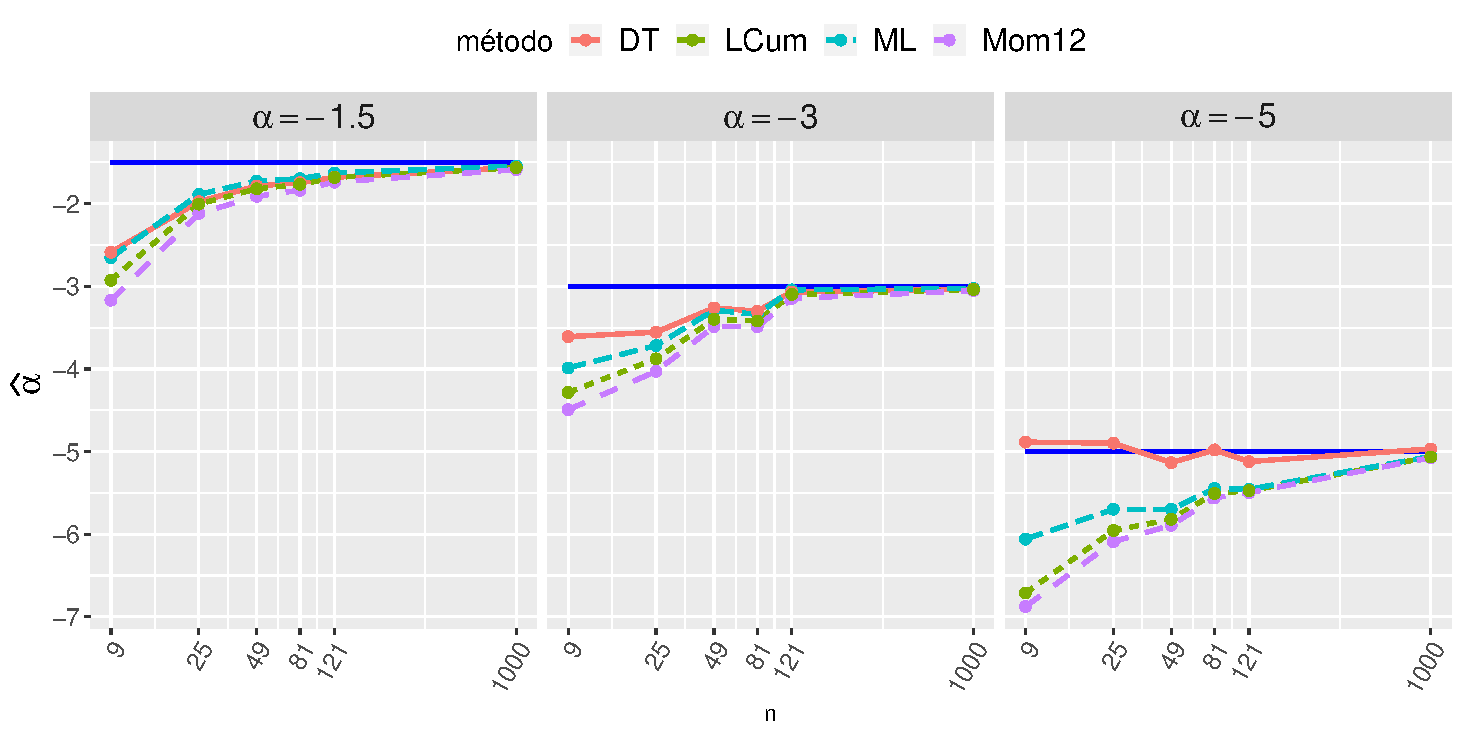
\includegraphics[width=.50\linewidth]{../../Figures/Tesis/Capitulo6/GraficoAlfaJstar2013_Cont_L=8Caso1.pdf}}
%	\subfigure[\label{ECMContJSTAR2013Caso1_L=8}$\widehat{\text{ECM}}$, L=8]{\includegraphics[width=.50\linewidth]{../../Figures/Tesis/Capitulo6/GraficoECMJstar2013_Cont_L=8Caso1.pdf}}
	\caption{\label{Caso1L1}\small Datos contaminados: Caso $1$, $\epsilon=0.01$ y $L=1$.}
\end{figure}

\begin{figure}[H]
%	\subfigure[\label{AlfasContJSTAR2013Caso1_L=1}$\widehat{\alpha}$, L=1]{\includegraphics[width=.48\linewidth]{../../Figures/Tesis/Capitulo6/GraficoAlfaJstar2013_Cont_L=1Caso1.pdf}}
%	\subfigure[\label{ECMContJSTAR2013Caso1_L=1}$\widehat{\text{ECM}}$ ,L=1]{\includegraphics[width=.48\linewidth]{../../Figures/Tesis/Capitulo6/GraficoECMJstar2013_Cont_L=1Caso1.pdf}}
	\subfigure[\label{AlfasContJSTAR2013Caso1_L=3}$\widehat{\text{Sesgo}}$]{\includegraphics[width=.48\linewidth]{../../Figures/Tesis/Capitulo6/GraficoSesgoJstar2013_Cont_L=3Caso1BarrasErrorypercentil.pdf}}
	\subfigure[\label{ECMContJSTAR2013Caso1_L=3}$\widehat{\text{ECM}}$]{\includegraphics[width=.48\linewidth]{../../Figures/Tesis/Capitulo6/GraficoECMJstar2013_Cont_L=3Caso1BarrasErrorypercentil.pdf}}
%	\subfigure[\label{AlfasContJSTAR2013Caso1_L=8}$\widehat{\alpha}$, L=8]{\includegraphics[width=.50\linewidth]{../../Figures/Tesis/Capitulo6/GraficoAlfaJstar2013_Cont_L=8Caso1.pdf}}
%	\subfigure[\label{ECMContJSTAR2013Caso1_L=8}$\widehat{\text{ECM}}$, L=8]{\includegraphics[width=.50\linewidth]{../../Figures/Tesis/Capitulo6/GraficoECMJstar2013_Cont_L=8Caso1.pdf}}
	\caption{\label{Caso1L3}\small Datos contaminados: Caso $1$, $\epsilon=0.01$ y $L=3$.}
\end{figure}

\begin{figure}[htb]
%	\subfigure[\label{AlfasContJSTAR2013Caso1_L=1}$\widehat{\alpha}$, L=1]{\includegraphics[width=.48\linewidth]{../../Figures/Tesis/Capitulo6/GraficoAlfaJstar2013_Cont_L=1Caso1.pdf}}
%	\subfigure[\label{ECMContJSTAR2013Caso1_L=1}$\widehat{\text{ECM}}$ ,L=1]{\includegraphics[width=.48\linewidth]{../../Figures/Tesis/Capitulo6/GraficoECMJstar2013_Cont_L=1Caso1.pdf}}
%	\subfigure[\label{AlfasContJSTAR2013Caso1_L=3}$\widehat{\alpha}$, L=3]{\includegraphics[width=.48\linewidth]{../../Figures/Tesis/Capitulo6/GraficoAlfaJstar2013_Cont_L=3Caso1.pdf}}
%	\subfigure[\label{ECMContJSTAR2013Caso1_L=3}$\widehat{\text{ECM}}$, L=3]{\includegraphics[width=.48\linewidth]{../../Figures/Tesis/Capitulo6/GraficoECMJstar2013_Cont_L=3Caso1.pdf}}
	\subfigure[\label{AlfasContJSTAR2013Caso1_L=8}$\widehat{\text{Sesgo}}$]{\includegraphics[width=.50\linewidth]{../../Figures/Tesis/Capitulo6/GraficoSesgoJstar2013_Cont_L=8Caso1BarrasErrorypercentil.pdf}}
	\subfigure[\label{ECMContJSTAR2013Caso1_L=8}$\widehat{\text{ECM}}$]{\includegraphics[width=.50\linewidth]{../../Figures/Tesis/Capitulo6/GraficoECMJstar2013_Cont_L=8Caso1BarrasErrorypercentil.pdf}}
	\caption{\label{Caso1L8}\small Datos contaminados: Caso $1$, $\epsilon=0.01$ y $L=8$.}
\end{figure}

%%%%%%%%%%%%%%%%%%%%%%%%%%%%%%%%%%%%%%%%%%%%%%%%%%%%%%%%%%%%%%%
%%% CASE 2, alpha_2 = -15, epsilon = 0.001, C = 100

Las figuras~\ref{Caso2L1},~\ref{Caso2L3} y~\ref{Caso2L8} presentan $\widehat{\alpha}$ y $\widehat{\text{ECM}}$ para el Caso $2$ de contaminación con $\epsilon=0.001$ y $C=100$. Este tipo de contaminación injecta un valor constante, en este caso $100$, con probabilidad $\epsilon=0.001$. Como estamos considerando muestras con media unitaria, este valor de $C$ respresenta un valor grande de contaminación. En este caso $\widehat\alpha_{\text{\tiny{DT}}}$ es, en media, más cercano al verdadero valor que los otros métodos, y el valor de $\widehat{\text{ECM}}$ es menor.

\begin{figure}[H]
	\subfigure[\label{AlfasContJSTAR2013Caso2_L=1}$\widehat{\text{Sesgo}}$]{\includegraphics[width=.48\linewidth]{../../Figures/Tesis/Capitulo6/GraficoSesgoJstar2013_Cont_L=1Caso1BarrasErrorypercentil.pdf}}
	\subfigure[\label{ECMContJSTAR2013Caso2_L=1}$\widehat{\text{ECM}}$]{\includegraphics[width=.48\linewidth]{../../Figures/Tesis/Capitulo6/GraficoECMJstar2013_Cont_L=1Caso1BarrasErrorypercentil.pdf}}
%	\subfigure[\label{AlfasContJSTAR2013Caso2_L=3}$\widehat{\alpha}$, L=3]{\includegraphics[width=.48\linewidth]{../../Figures/Tesis/Capitulo6/GraficoAlfaJstar2013_Cont_L=3Caso1.pdf}}
%	\subfigure[\label{ECMContJSTAR2013Caso2_L=3}$\widehat{\text{ECM}}$, L=3]{\includegraphics[width=.48\linewidth]{../../Figures/Tesis/Capitulo6/GraficoECMJstar2013_Cont_L=3Caso1.pdf}}
%	\subfigure[\label{AlfasContJSTAR2013Caso2_L=8}$\widehat{\alpha}$, L=8]{\includegraphics[width=.50\linewidth]{../../Figures/Tesis/Capitulo6/GraficoAlfaJstar2013_Cont_L=8Caso1.pdf}}
%	\subfigure[\label{ECMContJSTAR2013Caso2_L=8}$\widehat{\text{ECM}}$, L=8]{\includegraphics[width=.50\linewidth]{../../Figures/Tesis/Capitulo6/GraficoECMJstar2013_Cont_L=8Caso1.pdf}}
	\caption{\label{Caso2L1}\small Datos contaminados: Caso $2$, $\epsilon=0.001$ y $L=1$.}
\end{figure}

\begin{figure}[H]
%	\subfigure[\label{AlfasContJSTAR2013Caso2_L=1}$\widehat{\alpha}$, L=1]{\includegraphics[width=.48\linewidth]{../../Figures/Tesis/Capitulo6/GraficoAlfaJstar2013_Cont_L=1Caso1.pdf}}
%	\subfigure[\label{ECMContJSTAR2013Caso2_L=1}$\widehat{\text{ECM}}$ ,L=1]{\includegraphics[width=.48\linewidth]{../../Figures/Tesis/Capitulo6/GraficoECMJstar2013_Cont_L=1Caso1.pdf}}
	\subfigure[\label{AlfasContJSTAR2013Caso2_L=3}$\widehat{\text{Sesgo}}$, L=3]{\includegraphics[width=.48\linewidth]{../../Figures/Tesis/Capitulo6/GraficoSesgoJstar2013_Cont_L=3Caso1BarrasErrorypercentil.pdf}}
	\subfigure[\label{ECMContJSTAR2013Caso2_L=3}$\widehat{\text{ECM}}$, L=3]{\includegraphics[width=.48\linewidth]{../../Figures/Tesis/Capitulo6/GraficoECMJstar2013_Cont_L=3Caso1BarrasErrorypercentil.pdf}}
%	\subfigure[\label{AlfasContJSTAR2013Caso2_L=8}$\widehat{\alpha}$, L=8]{\includegraphics[width=.50\linewidth]{../../Figures/Tesis/Capitulo6/GraficoAlfaJstar2013_Cont_L=8Caso1.pdf}}
%	\subfigure[\label{ECMContJSTAR2013Caso2_L=8}$\widehat{\text{ECM}}$, L=8]{\includegraphics[width=.50\linewidth]{../../Figures/Tesis/Capitulo6/GraficoECMJstar2013_Cont_L=8Caso1.pdf}}
	\caption{\label{Caso2L3}\small Datos contaminados: Caso $2$, $\epsilon=0.001$ y $L=3$.}
\end{figure}

\begin{figure}[H]
%	\subfigure[\label{AlfasContJSTAR2013Caso2_L=1}$\widehat{\alpha}$, L=1]{\includegraphics[width=.48\linewidth]{../../Figures/Tesis/Capitulo6/GraficoAlfaJstar2013_Cont_L=1Caso1.pdf}}
%	\subfigure[\label{ECMContJSTAR2013Caso2_L=1}$\widehat{\text{ECM}}$ ,L=1]{\includegraphics[width=.48\linewidth]{../../Figures/Tesis/Capitulo6/GraficoECMJstar2013_Cont_L=1Caso1.pdf}}
%	\subfigure[\label{AlfasContJSTAR2013Caso2_L=3}$\widehat{\alpha}$, L=3]{\includegraphics[width=.48\linewidth]{../../Figures/Tesis/Capitulo6/GraficoAlfaJstar2013_Cont_L=3Caso1.pdf}}
%	\subfigure[\label{ECMContJSTAR2013Caso2_L=3}$\widehat{\text{ECM}}$, L=3]{\includegraphics[width=.48\linewidth]{../../Figures/Tesis/Capitulo6/GraficoECMJstar2013_Cont_L=3Caso1.pdf}}
	\subfigure[\label{AlfasContJSTAR2013Caso2_L=8}$\widehat{\text{Sesgo}}$, L=8]{\includegraphics[width=.45\linewidth]{../../Figures/Tesis/Capitulo6/GraficoSesgoJstar2013_Cont_L=8Caso1BarrasErrorypercentil.pdf}}
	\subfigure[\label{ECMContJSTAR2013Caso2_L=8}$\widehat{\text{ECM}}$, L=8]{\includegraphics[width=.45\linewidth]{../../Figures/Tesis/Capitulo6/GraficoECMJstar2013_Cont_L=8Caso1BarrasErrorypercentil.pdf}}
	\caption{\label{Caso2L8}\small Datos contaminados: Caso $2$, $\epsilon=0.001$  y $L=8$.}
\end{figure}
%%% CASE 3, epsilon 0.001, k = 2

Las figuras~\ref{Caso3L1},~\ref{Caso3L3} y~\ref{Caso3L8} muestran $\widehat{\alpha}$ y $\widehat{\text{ECM}}$ para el Caso 3 de contaminación con $\epsilon=0.005$ y $k=2$. En este caso se contamina la muestra proveniente del modelo verdadero con un observaciones que, con probabilidad $\epsilon=0.005$, provienen de una distribución $\mathcal G_I^0$ con un factor de escala cien veces más grande que el correspondiente al modelo verdadero. El comportamiento de estos estimadores sigue el mismo patrón para $L=3 \text{ y } 8$, $\widehat\alpha_{\text{DT}}$ produce estimaciones más cercanas al verdadero valor con un ECM más chico. No hay un buen estimador para el caso $L=1$ en este caso de contaminación.

\begin{figure}[h!]
	\subfigure[\label{AlfasContJSTAR2013Caso3_L=1}$\widehat{\text{Sesgo}}$]{\includegraphics[width=.45\linewidth]{../../Figures/Tesis/Capitulo6/GraficoSesgoJstar2013_Cont_L=1Caso3BarrasErrorypercentil.pdf}}
	\subfigure[\label{ECMContJSTAR2013Caso3_L=1}$\widehat{\text{ECM}}$]{\includegraphics[width=.45\linewidth]{../../Figures/Tesis/Capitulo6/GraficoECMJstar2013_Cont_L=1Caso3BarrasErrorypercentil.pdf}}
%	\subfigure[\label{AlfasContJSTAR2013Caso3_L=3}$\widehat{\alpha}$, L=3]{\includegraphics[width=.48\linewidth]{../../Figures/Tesis/Capitulo6/GraficoAlfaJstar2013_Cont_L=3Caso3.pdf}}
%	\subfigure[\label{ECMContJSTAR2013Caso3_L=3}$\widehat{\text{ECM}}$, L=3]{\includegraphics[width=.48\linewidth]{../../Figures/Tesis/Capitulo6/GraficoECMJstar2013_Cont_L=3Caso3.pdf}}
%	\subfigure[\label{AlfasContJSTAR2013Caso3_L=8}$\widehat{\alpha}$, L=8]{\includegraphics[width=.50\linewidth]{../../Figures/Tesis/Capitulo6/GraficoAlfaJstar2013_Cont_L=8Caso3.pdf}}
%	\subfigure[\label{ECMContJSTAR2013Caso3_L=8}$\widehat{\text{ECM}}$, L=8]{\includegraphics[width=.50\linewidth]{../../Figures/Tesis/Capitulo6/GraficoECMJstar2013_Cont_L=8Caso3.pdf}}
	\caption{\label{Caso3L1}\small Datos contaminados: Caso $3$, $\epsilon=0.005$ y $ L=1$.}
\end{figure}

\begin{figure}[h!]
%	\subfigure[\label{AlfasContJSTAR2013Caso3_L=1}$\widehat{\alpha}$, L=1]{\includegraphics[width=.48\linewidth]{../../Figures/Tesis/Capitulo6/GraficoAlfaJstar2013_Cont_L=1Caso3.pdf}}
%	\subfigure[\label{ECMContJSTAR2013Caso3_L=1}$\widehat{\text{ECM}}$ ,L=1]{\includegraphics[width=.48\linewidth]{../../Figures/Tesis/Capitulo6/GraficoECMJstar2013_Cont_L=1Caso3.pdf}}
	\subfigure[\label{AlfasContJSTAR2013Caso3_L=3}$\widehat{\text{Sesgo}}$]{\includegraphics[width=.48\linewidth]{../../Figures/Tesis/Capitulo6/GraficoSesgoJstar2013_Cont_L=3Caso3BarrasErrorypercentil.pdf}}
	\subfigure[\label{ECMContJSTAR2013Caso3_L=3}$\widehat{\text{ECM}}$]{\includegraphics[width=.48\linewidth]{../../Figures/Tesis/Capitulo6/GraficoECMJstar2013_Cont_L=3Caso3BarrasErrorypercentil.pdf}}
%	\subfigure[\label{AlfasContJSTAR2013Caso3_L=8}$\widehat{\alpha}$, L=8]{\includegraphics[width=.50\linewidth]{../../Figures/Tesis/Capitulo6/GraficoAlfaJstar2013_Cont_L=8Caso3.pdf}}
%	\subfigure[\label{ECMContJSTAR2013Caso3_L=8}$\widehat{\text{ECM}}$, L=8]{\includegraphics[width=.50\linewidth]{../../Figures/Tesis/Capitulo6/GraficoECMJstar2013_Cont_L=8Caso3.pdf}}
	\caption{\label{Caso3L3}\small Datos contaminados: Caso $3$, $\epsilon=0.005$ y $ L=3$.}
\end{figure}

\begin{figure}[htb]
%	\subfigure[\label{AlfasContJSTAR2013Caso3_L=1}$\widehat{\alpha}$, L=1]{\includegraphics[width=.48\linewidth]{../../Figures/Tesis/Capitulo6/GraficoAlfaJstar2013_Cont_L=1Caso3.pdf}}
%	\subfigure[\label{ECMContJSTAR2013Caso3_L=1}$\widehat{\text{ECM}}$ ,L=1]{\includegraphics[width=.48\linewidth]{../../Figures/Tesis/Capitulo6/GraficoECMJstar2013_Cont_L=1Caso3.pdf}}
%	\subfigure[\label{AlfasContJSTAR2013Caso3_L=3}$\widehat{\alpha}$, L=3]{\includegraphics[width=.48\linewidth]{../../Figures/Tesis/Capitulo6/GraficoAlfaJstar2013_Cont_L=3Caso3.pdf}}
%	\subfigure[\label{ECMContJSTAR2013Caso3_L=3}$\widehat{\text{ECM}}$, L=3]{\includegraphics[width=.48\linewidth]{../../Figures/Tesis/Capitulo6/GraficoECMJstar2013_Cont_L=3Caso3.pdf}}
	\subfigure[\label{AlfasContJSTAR2013Caso3_L=8}$\widehat{\text{Sesgo}}$]{\includegraphics[width=.50\linewidth]{../../Figures/Tesis/Capitulo6/GraficoSesgoJstar2013_Cont_L=8Caso3BarrasErrorypercentil.pdf}}
	\subfigure[\label{ECMContJSTAR2013Caso3_L=8}$\widehat{\text{ECM}}$]{\includegraphics[width=.50\linewidth]{../../Figures/Tesis/Capitulo6/GraficoECMJstar2013_Cont_L=8Caso3BarrasErrorypercentil.pdf}}
	\caption{\label{Caso3L8}\small Datos contaminados: Caso $3$, $\epsilon=0.005$ y $ L=8$.}
\end{figure}

Como se mencionó anteriormente, los algoritmos implementados para los casos de los estimadores Mom12 y Logcumulante no convergen en algunos casos. En el experimento Monte Carlo, si Mom12 o  Logcumulante no convergen, no consideramos esta iteración al momento de estimar, por lo que la cantidad de elementos para calcular $\overline{\widehat{\alpha}}$, el sesgo y el error cuadrático medio es un poco menor que $1000$.

La tabla~\ref{tabla_removidos} informa, a modo de ejemplo, el porcentaje de casos que fueron removidos para el Caso $1$ y $\alpha_2 = -15, \epsilon = 0.01$. Estos resultados son consistentes con los otros escenarios de contaminación, y sugieren que estos métodos son progresivamente más propensos a fallar en casos con mayor presencia de ruido speckle.

\begin{table}[H]
	\centering
	\begin{tabular}{c S[table-format=2.2]S[table-format=2.2]}
		\toprule
		\mc{$L$} & \mc{Mom12}  & \mc{LC} \\
		\midrule
		1 & 22.87  & 21.56 \\
		3 & 11.71  &  11.87 \\
		8 & 5.81   & 6.04  \\
		\bottomrule
	\end{tabular}
\caption{\label{tabla_removidos}Porcentaje de casos de no convergencia para los estimadores de Momentos y  Logcumulante en el Caso 1, $\alpha_2 = -15, \epsilon = 0.01$}
\end{table}


%\begin{figure}[h!]
%	\centering
%	\subfigure[\label{AlfasContJSTAR2013Caso1_L=1}$\widehat{\alpha}$]{\includegraphics[width=.48\linewidth]{../../Figures/Tesis/Capitulo6/GraficoAlfaJstar2013_Cont_L=1Caso1.pdf}}
%	\subfigure[\label{ECMContJSTAR2013Caso1_L=1}ECM]{\includegraphics[width=.48\linewidth]{../../Figures/Tesis/Capitulo6/GraficoECMJstar2013_Cont_L=1Caso1.pdf}}
%	\caption{\small Datos contaminados: Caso1, L=1.}
%\end{figure}
%
%\begin{figure}[h!]
%	\centering
%	\subfigure[\label{AlfasContJSTAR2013Caso1_L=3}$\widehat{\alpha}$]{\includegraphics[width=.47\linewidth]{../../Figures/Tesis/Capitulo6/GraficoAlfaJstar2013_Cont_L=3Caso1.pdf}}
%	\subfigure[\label{ECMContJSTAR2013Caso1_L=3}ECM]{\includegraphics[width=.47\linewidth]{../../Figures/Tesis/Capitulo6/GraficoECMJstar2013_Cont_L=3Caso1.pdf}}
%	\caption{\small Datos contaminados: Caso1, L=3.}
%\end{figure}
%
%\begin{figure}[h!]
%	\centering
%	\subfigure[\label{AlfasContJSTAR2013Caso1_L=8}$\widehat{\alpha}$]{\includegraphics[width=.47\linewidth]{../../Figures/Tesis/Capitulo6/GraficoAlfaJstar2013_Cont_L=8Caso1.pdf}}
%	\subfigure[\label{ECMContJSTAR2013Caso1_L=8}ECM]{\includegraphics[width=.47\linewidth]{../../Figures/Tesis/Capitulo6/GraficoECMJstar2013_Cont_L=8Caso1.pdf}}
%	\caption{\small Datos contaminados: Caso1, L=8.}
%\end{figure}
%\begin{figure}[h!]
%	\centering
%	\subfigure[\label{AlfasEstimadosJSTAR2013_L=3}$\widehat{\alpha}$]{\includegraphics[width=.47\linewidth]{../../Figures/Tesis/Capitulo6/GraficoAlfaJstar2013NoContL=3.pdf}}
%	\subfigure[\label{ECMEstimadosJSTAR2013_L=3}ECM]{\includegraphics[width=.47\linewidth]{../../Figures/Tesis/Capitulo6/GraficoECMJstar2013NoContL=3.pdf}}
%	\caption{\small  Datos sin contaminar, L=3.}
%\end{figure}
%
%\begin{figure}[h!]
%	\subfigure[\label{AlfasEstimadosJSTAR2013_L=8}$\widehat{\alpha}$]{\includegraphics[width=.47\linewidth]{../../Figures/Tesis/Capitulo6/GraficoAlfaJstar2013NoContL=8.pdf}}
%	\subfigure[\label{ECMEstimadosJSTAR2013_L=8}ECM]{\includegraphics[width=.47\linewidth]{../../Figures/Tesis/Capitulo6/GraficoECMJstar2013NoContL=8.pdf}}
%	\caption{\small Datos sin contaminar, L=8.}
%\end{figure}
\subsection{Aplicación a una imagen real}

Hemos aplicado estos métodos a una imagen real, la misma imagen utilizada en \citet{APSAR2013ParameterEstimationStochasticDistances}, una imagen E-SAR de un look de los alrededores de Munich, banda L, polarización HH en formato intensidad, como se indica en \citet{Horn1996}. La figura~\ref{reales2} muestra las regiones usadas para estimar el parámetro de textura. Esta imagen tiene $300\times250$ pixels y comprende principalmente dos áreas de cultivo diferentes.

\begin{figure}[htb]
	\centering
	\includegraphics[width=.52\linewidth,angle=-90]{../../Figures/Tesis/Capitulo6/MunchCortadaReg.pdf}
	\caption{\label{reales2}Image real E-SAR junto con la regiones usadas para estimar el parámetro $\alpha$.}
\end{figure}

La tabla~\ref{resultadosalfaEstim} muestra los resultados de las estimaciones del parámetro $\alpha$ para cada región rectangular junto con los tiempos de procesamiento, donde $NA$ significa que el algoritmo correspondiente no convergió. El resto de las estimaciones arrojan valores compatibles con el mismo tipo de zona en cada una de las muestras analizadas. 

\begin{table}[htb]
	\centering
	\begin{tabular}{c*9{c}}
		\toprule
		\multirow{2 }{*} {Color} & \multirow{2 }{*}{n} & \multirow{2 }{*}{$\widehat{\alpha}_{\text{\tiny{MV}}}$} & \multirow{2 }{*}{$\widehat\alpha_{\text{\tiny{DT}}}$} & \multirow{2 }{*}{$\widehat\alpha_{\text{\tiny{Mom12}}}$} & \multirow{2 }{*}{$\widehat\alpha_{\text{\tiny{LC}}}$} & \small Tiempo  &  \small Tiempo & \small Tiempo &  \small Tiempo  \\
		&      &                        &                           &                                 &                                &  \small MV &  \small DT &   \small Mom12 &  LC \\
		\midrule
		Magenta   & $100$  & $-1.9$ & $-2.7$ & $-1.9$  & $-1.7$  & $0.03$ & $5.85$ & $0.03$  & $0.02$\\
		Amarillo  & $90$   & $-6.2$ & $-5.1$ & $-6.6$  & $-6.8$  & $0.00$ &$5.16$  & $0.00$  & $0.00$\\
		Rojo      & $64$   & $-1.8$ & $-1.9$ & $-1.9$  & $-1.8$  & $ 0.00 $&$4.17$ & $0.00$  & $0.00$\\
		Verde     & $48$   & $-2.5$ & $-2.5$ & $-2.9$  & $-3.1$  & $0.00$ & $3.31$ & $ 0.00$ & $0.00$\\
		Azul      & $25$   & $-4.9$ & $-3.0$ &  $NA$   & $NA$    & $0.00$ & $2.08$ & $0.00$  & $0.00$\\
		\bottomrule
	\end{tabular}
\caption{\label{resultadosalfaEstim}$\widehat{\alpha}$ para las muestras de la figura~\ref{reales2}.}
\end{table}

%Aplicamos el test de Kolmogorov-Smirnov (KS-test) como otra estrategia para evaluar a los estimadores bajo estudio. Se aplicó el test a dos muestras: una muestra $\bm x$ que proviene de la imagen, y una segunda muestra $\bm y$ simulada.
%Babu and Feigelson \citet{Jogesh2006} alertan sobre el uso de la misma muestra para estimar los parámetros y para realizar el KS test, porque se pueden sacar conclusiones erróneas. Entonces tomamos una muestra de la imagen real $\bm x$ usada para estimar los parámetros con los cuatro métodos bajo análisis y la comparamos con una muestra simulada $\bm y$, del mismo tamaño, proveniente de una distribución $\mathcal G_I^0$ con los parámetros estimados. Se aplicó el KS test entre $\bm x$ y $\bm y$ considerando la hipótesis nula $H_0$ ``ambas muestras provienen de la misma distribución'', y el complemento de esta hipótesis como hipótesis alternativa.
%
%La tabla~\ref{resultadosTestMunich} muestra los $p$-valores. Se puede observar que no hay suficiente evidencia para rechazar la hipótesis nula con un nivel de signficación del $5$\% en ninguno de los casos.

%\begin{table}[h!]
%	\centering
%	\begin{tabular}{c*4{c}}
%		\toprule
%		Color      & TestMV    & TestDT    & TestMom12  &TestLC \\
%		\midrule
%		Magenta    & $0.46$    & $ 0.58$   & $0.28$   & $0.69$\\
%		Amarillo   & $0.63$    & $0.98$    & $0.76$   & $0.22$\\
%		Rojo       & $0.30$    & $ 0.30$   & $0.21$   & $0.99$\\
%		Verde      & $0.37$    & $0.85$    & $0.37$   & $0.37$\\
%		Azul       & $0.15$    & $0.07$    & $NA $    & $NA $\\
%		\bottomrule
%	\end{tabular}
%\caption{\label{resultadosTestMunich} $p$-valor del KS test para las muestras de la imagen de la figura~\ref{reales2}.}
%\end{table}

La figura~\ref{ImagenCornerReflector} muestra una imagen con la presencia de un corner reflector, mientras que la figura~\ref{MuestrasCorner} muestra las regiones usadas para estimar el parámetro de textura para esta situación. La tabla~\ref{resultadosCorner} presenta los valores de  $\widehat{\alpha}$ para cada área rectangular en la imagen de la figura~\ref{MuestrasCorner}.

Los estimadores MV, Mom12 y  Logcumulantes son incapaces de producir una estimación en pequeñas muestras.  Se puede observar que tanto $\widehat\alpha_{\text{\tiny{Mom12}}}$ como $\widehat\alpha_{\text{\tiny{LC}}}$ requieren al menos un tamaño de muestra de $90$ observaciones para que se pueda dar una estimación para $\alpha$. El estimador basado en la distancia triangular produce valores plausibles bajo contaminación incluso con muestras muy pequeñas y produce estimaciones más estables que las dadas por MV.

\begin{figure}[htb]
	\centering
	\includegraphics[angle =90,width=.8\linewidth]{../../Figures/Tesis/Capitulo6/Corner.pdf}
	\caption{\label{ImagenCornerReflector} Imagen real SAR de $1$-look con un corner reflector.}
\end{figure}

\begin{figure}[htb]
	\centering
	%\subfigure[Single-look E-SAR imagen con un corner reflector.]{\includegraphics[angle =90,width=.8\linewidth]{../../Figures/Tesis/Capitulo6/Corner.pdf}}
	%\subfigure[\label{Cornerregiones} Regiones de interés.]{\includegraphics[angle =90,width=.8\linewidth,]{../../Figures/Tesis/Capitulo6/CornerReg}}
	\includegraphics[angle =90,width=.8\linewidth,]{../../Figures/Tesis/Capitulo6/CornerReg}
	\caption{\label{MuestrasCorner} Muestras de varios tamaños en una imagen real SAR de $1$-look con un corner reflector.}
\end{figure}

\begin{table}[htb]
	\centering
	\caption{\label{resultadosCorner}$\widehat{\alpha}$ y tiempos de procesos para las muestras presentadas en la figura~\ref{MuestrasCorner}}
	\begin{tabular}{c c r*7{r}}
	%\begin{tabular}{c c S[table-number-alignment = center] S[table-number-alignment = center] S S S S S}
	\toprule
	\multirow{2 }{*} {Color} & \multirow{2 }{*}{n} & \multirow{2 }{*}{$\widehat\alpha_{\text{\tiny{MV}}}$} & \multirow{2 }{*}{$\widehat\alpha_{\text{\tiny{DT}}}$} & \multirow{2 }{*}{$\widehat\alpha_{\text{\tiny{Mom12}}}$} & \multirow{2 }{*}{$\widehat\alpha_{\text{\tiny{LC}}}$} & \small Tiempo  &  \small Tiempo & \small Tiempo &  \small Tiempo  \\
	&      &                        &                           &                                 &                                &  \mc{\small{MV}} &  \mc{\small{DT}} &  \mc{\small{Mom12}} &  \mc{\small{LC}} \\
	\midrule
		Magenta     & $15$  & $-20.0$ & $-4.1$  & $NA $   & $NA $     &  $0.03$  &  $1.95$      &  $0.03$   &  $0.03$ \\
		Verde       & $42$  & $-9.2$  & $-5.0$  & $NA$    & $ NA $    &  $0.00$  &  $4.04$      &  $0.00$   &  $0.00$\\
		Azul        & $90$  & $-3.5$  & $-2.7$  & $-4.7$  & $-14.2$   &  $0.02$  &  $4.85$      &  $0.00$   &  $0.00$\\
		Amarillo    & $156$ & $-2.2$  & $-1.8$  & $-2.6$  & $-3.4$    &  $0.01$  &  $8.35$      &  $0.00$   &  $0.00$\\
		Rojo        & $225$ & $-1.9$ & $-1.7$  & $-2.1$   & $-2.5$    &  $0.02$  &  $10.97$     &  $0.00$   &  $0.00$\\
		\bottomrule
	\end{tabular}
\end{table}

%\begin{table}[htb]
%	\centering
%	\caption{\label{resultadosCorner}$\widehat{\alpha}$ y tiempos de procesos para las muestras presentadas en la figura~\ref{MuestrasCorner}}
%	%\begin{tabular}{c*9{c}}
%	\begin{tabular}{c c D{.}{,}{-1} }
%		\toprule
%		\multirow{2 }{*} {Color} & \multirow{2 }{*}{n} & \multirow{2 }{*}{$\widehat\alpha_{\text{\tiny{MV}}}$} \\
%		\midrule
%		Magenta     & $15$  & $-20.0$ \\
%		Verde       & $42$  & $-9.2$  \\
%		Azul        & $90$  & $-3.5$  \\
%		Amarillo    & $156$ & $-2.2$  \\
%		Rojo        & $225$ & $-1.9$ \\
%		\bottomrule
%	\end{tabular}
%\end{table}

%La tabla~\ref{pvaluesTrueNestedSamples} presenta los $p$-valores del KS test aplicado a las muestras señaladas en la figura~\ref{MuestrasCorner}. Como se mencionó anteriormente el $\widehat\alpha_{\text{Mom12}}$ y $\widehat\alpha_{\text{LC}}$ no pudieron producir estimaciones en dos muestras y, por lo tanto, no fue posible aplicar el test. Cabe señalar que  se rechaza la hipótesis nula: las muestras provienen de la misma distribución, para la muestra azul y el MV estimador, y para la muestra roja que es la de mayor tamaño para los estimadores $\widehat\alpha_{\text{Mom12}}$ y $\widehat\alpha_{\text{LC}}$. 

Estos resultados nos llevan a concluir que la distribución $\mathcal{G}_I^0$ es una buena opción para modelar adecuadamente datos provenientes de imágenes SAR con datos de intensidad ante la presencia de contaminación. Asimismo podemos concluir que el estimador propuesto es una buena elección para estimar el parámetro de textura de la distribución $\mathcal{G}_I^0$, ya que es competitivo frente al MV estimador para datos sin contaminar, incluso mejora su desempeño en alguno de los casos estudiados. Además mejora a los otros dos estimadores evauados especialmente para el caso de muestras de pequeño tamaño. Al momento de estimar el parámetro de textura en una imagen real el  $\widehat\alpha_{\text{\tiny{DT}}}$ es el estimador que arrojó valores estimados más estables frente a la presencia de un corner reflector.

%\begin{table*}[htb]
%	\centering
%	\caption{\label{pvaluesTrueNestedSamples} $p$-valores del KS test para la muestras indicadas en la figura~\ref{MuestrasCorner}.}
%	\begin{tabular}{c*4{r}}
%		\toprule
%		Color       &  TestMV    &  TestDT    &  TestMom12  &  TestLC\\
%		\midrule
%		Magenta     & $ 0.38$    & $ 0.93 $   & $ NA $     & $  NA$\\
%		Verde       & $ 0.11$    & $ 0.93$    & $ NA $     & $   NA$\\
%		Azul        & $ 0.01 $   & $0.11 $    & $ 0.40$    & $ 0.11$\\
%		Amarillo    & $0.19$     & $0.31$     & $ 0.46 $   & $0.15$\\
%		Rojo        & $0.23$     & $0.12$     & $ 0.008$   & $0.02$\\
%		\bottomrule
%	\end{tabular}
%\end{table*}
%\begin{table}[hbt]
%	\centering
%	\caption{Número de casos de no convergencia para distancia triangular generalizada, L=$3$}
%	\label{NoConvDTG}
%		\begin{tabular}{c*7{r}}
%			\toprule		
%			$\alpha$ & $n$ & s=$1$ & s=$1.5$ & s=$2$ & s=$3$ & s=$4$\\
%			\midrule
%			\multirow{3 }{*}{$-1.5$} 
%			& $9$  & $26$ & $14$ & $11$ & $7$ & $6$ \\ 
%			& $25$ & $0 $ & $0 $ & $0$  & $0$ & $0$\\ 
%			& $49$ & $0$  & $1 $ & $1$  & $0$ & $0$\\ 
%			\midrule
%			\multirow{3 }{*}{$-3$}
%			& $9$  & $10$ & $6 $ & $5$  & $4$ & $4$ \\ 
%			& $25$ & $0$  & $1 $ & $1$  & $1$ & $0$\\ 
%			& $49$ & $0$  & $0$  & $0$  & $0$ & $0$\\ 
%			\midrule
%			\multirow{3 }{*}{$-5$} 
%			& $9$  & $4 $ & $3 $ & $3$  & $2$ & $1$\\ 
%			& $25$ & $1 $ & $1 $ & $1$  & $0$ & $0$\\ 
%			& $49$ & $0$  & $0 $ & $0$  & $0$ & $0$\\ 
%			\midrule
%			\multirow{3 }{*}{$-8$} 
%			& $0$ & $0$ & $0$ & $0$  & $0$ & $0$\\ 
%			& $0$ & $0$ & $0$ & $0$  & $0$ & $0$\\ 
%			& $0$ & $0$ & $0$ & $0$  & $0$ & $0$\\ 
%			\midrule
%			\bottomrule 	
%		\end{tabular}
%\end{table}	

\section{Mejorando la propuesta}
\label{mejorando}

Para el caso $L=1$ la distribución $\mathcal{G}_I^0(\alpha,\gamma)$ es una distribución de Pareto Generalizada de parámetros $\mathcal{PG}(\mu,\sigma,\beta)$, donde $\mu=0$, $\sigma=\gamma$ y $\beta=-\alpha$. El parámetro de textura de la distribución $\mathcal{G}$ está relacionado con el índice de la cola. En el trabajo que presentamos en \citet{Chan2016} empleamos teoría de valores extremos para proponer un estimador para este parámetro. Por este motivo en esta tesis continuamos el análisis para el caso multilook.

En \citet{gambini2015} presentamos el MDE estimador utilizando distancia triangular y encontrando el mínimo recorriendo valores en una grilla, estimando $\widehat{f}_{\text{\tiny{A}}_n}$ con núcleo IG y proponiendo un valor de ancho de banda $b$ encontrado empíricamente.

En esta sección proponemos mejoras:

\begin{itemize}
	\item Consideramos otros núcleos.% estudiando el MISE que se presentó en la subsección~\ref{MISE}.
	\item Utilizamos el método LSCV para encontrar el ancho de banda que se presentó en la ecuación~\eqref{LSCV}.
	\item Utilizamos el algoritmo L-BFGS-B presentado en la sección~\ref{jstar} para encontrar el estimador $\widehat{\alpha}_{\text{\tiny{DT}}}$ minimizando la distancia definida en la ecuación~\eqref{minimization}.
	\item Contamos casos de no convergencia de los algoritmos numéricos empleados, entendiendo que un algoritmo no converge si devuelve como valor estimado del parámetro a alguno de los extremos del intervalo de búsqueda.
\end{itemize}  

La pregunta es ¿por qué el núcleo $IG$ y no otro? ¿Cómo elegir el mejor núcleo? Para responder a estas preguntas estudiamos otros núcleos. En la sección~\ref{NucleosAsimetricos} se mencionó que, dentro de los núcleos más estudiados, se encuentran los núcleos IG, $\Gamma^1$, $\Gamma^2$ y LN. En \citet{gambini2015} evaluamos la performance del núcleo IG, en esta sección vamos a evaluar los otros dos núcleos y compararemos su performance con el núcleo IG. 

En una primera instancia estimamos el MISE~\eqref{MISE} ($\widehat{\text{MISE}}$) para cada núcleo estudiado, para distintas combinaciones de los parámetros, tamaños muestrales y número de looks. 

Realizamos $500$ replicaciones, en cada replicación generamos una muestra proveniente de una distribución $\mathcal{G}_I^0(\alpha,\gamma^*,L)$ y calculamos 
\begin{align}
\label{MiseEst}
\widehat{\text{MISE}}=\dfrac{1}{500} \sum_{i=1}^{500}\int_0^{+\infty} (\widehat{f}_{b,\text{K}}^i(x)-f(x))^2 dx,
\end{align}
donde $\widehat{f}_{b,\text{K}}^i(x)$ es el estimador de la función de densidad subyacente en la replicación $i$ para el núcleo $\text{K}$, que depende del ancho de banda $\text{b}$.

En la tabla~\ref{MiseyCantCasosNoConvergenciaL=3} se muestran los valores de $\widehat{\text{MISE}}$ para $\alpha=\{-1.5,-3,-5,-8\}$, $L=3$, $\gamma^*=-\alpha-1$, $n=\{9,25,49,81,121\}$ y $\text{K}=\{\Gamma^1,\Gamma^2,\text{LN},\text{IG},\text{IGJstar\}}$, donde $\Gamma^1$, $\Gamma^2$, LN, IG, IGJstar corresponden a los núcleos $\Gamma^1$, $\Gamma^2$, LN e IGo respectivamente. La columna IGJstar corresponde al núcleo estudiado en \citet{gambini2015} donde se consideró un ancho de banda fijo encontrado empíricamente. En esta oportunidad se aplicó el método LSCV para encontrar el ancho de banda en cada replicación y para cada combinación de los parámetros en el resto de los núcleos estudiados.

Se puede observar que:
\begin{itemize}
	\item Los valores del MISE son muy similares para los núcleos $\Gamma^1$ y $\Gamma^2$, por lo que se eligió el núcleo $\Gamma^1$ ya que presenta menor MISE en la mayoría de los casos planteados. A partir de ahora el núcleo $\Gamma^1$ se llamará $\Gamma$.
	\item Los valores del $\widehat{\text{MISE}}$ correspondientes a los núcleos IG y con IGJstar son de varios órdenes de magnitud mayor a los otros núcleos.
\end{itemize} 

Luego evaluamos la cantidad de casos de no convergencia de cada método. La tabla~\ref{MiseyCantCasosNoConvergenciaL=3} muestra el porcentaje de casos donde el valor de $\widehat{\alpha}=-20$, no se observaron situaciones donde $\widehat{\alpha}=-1.$ En negrita están marcados los casos donde se presentan el mayor porcentaje. Se puede observar que, en general, el núcleo IG es el que presenta mayor porcentaje de ocurrencias de no convergencia.

Además estudiamos el sesgo y el ECM para el caso donde el número de looks es $L=3$, la tabla~\ref{SesgoyECMSinContConConstL=3} muestra los resultados obtenidos. En negrita están marcados los casos donde el sesgo y el ECM son menores con IG e IGJstar respecto de los núcleos $\Gamma$ y LN. Se puede observar que la performance de estos dos últimos núcleos  mejora al núcleo IG (en sus dos versiones) en la mayoría de los casos analizados. Sin embargo IG muestra una menor variabilidad salvo para zonas extremadamente texturadas, lo que no sucede con IGJstar. 

Entonces, priorizando la calidad del ajuste, el porcentaje de casos de convergencia y el sesgo continuamos el análisis con los núcleos $\Gamma$ y LN.

\begin{table}[hbt]										
	\centering									
	\small									
	\begin{tabular}{cc|SSSSS|SSSS}									
		\toprule									
		\multirow{3 }{*}{$\alpha$} &\multirow{3 }{*}{ n  } & \multicolumn{5}{c|}{\multirow{2 }{*}{MISE}} & \multicolumn{4}{c}{Porcentaje de casos de}\\
		&  &            &            &    &    &         &   \multicolumn{4}{c}{no convergencia}\\
		%\multirow{3 }{*}{$\alpha$} &\multirow{3 }{*}{ n  } & \multirow{2 }{*}{\multicolumn{5}{c|}{Mise}} & \multirow{2 }{*}{\multicolumn{4}{c}}{Cantidad de casos de}\\
		
		\cmidrule(r){3-7}
		\cmidrule(r){8-11}
		%\midrule
		
		&  & \mc{$\Gamma^1$} & \mc{$\Gamma^2$} & \mc{LN} & \mc{IG} & \multicolumn{1}{c|}{IGJstar}  & $\Gamma$ & \mc{LN} & \mc{IG} & \mc{IGJstar}  \\
		\midrule				
		\multirow{5 }{*}{$-1.5$} 
		 &   9    	&  	  0.407  	&	  0.411  	&	  0.811  	&	  6.119   	&	  41.330  	&	 0 	&	 0.4 	&	 0.4 	&	 0  \\
		 &   25   	&  	  0.123  	&	  0.145  	&	  0.184  	&	  2.464   	&	  17.024  	&	 0 	&	 0 		&	 0 		&	 0  \\
		 &   49   	&  	  0.082  	&	  0.100  	&	  0.538  	&	  1.157   	&	  9.671  	&	 0 	&	 0 		&	 0 		&	 0  \\
		 &   81   	&  	  0.064  	&	  0.079  	&	  0.085  	&	  0.753   	&	  6.126  	&	 0 	&	 0 		&	 0 		&	 0  \\
		 &   121  	&  	  0.064  	&	  0.076  	&	  0.081  	&	  0.528   	&	  4.000  	&	 0 	&	 0 		&	 0 		&	 0  \\
		\cmidrule(r){1-7}
		 \cmidrule(r){8-11}									
		 \multirow{5 }{*}{$-3$}	
		 &   9    	&  	  0.253  	&	  0.273  	&	  0.563  	&	  12.473  	&	  50.020  	&	 5.2 &	 7.2 	&  \textbf{8} 	&  6.8  \\
		 &   25   	&  	  0.080  	&	  0.093  	&	  0.106  	&	  3.217   	&	  25.401  	&	 0.2  &	 1 		&	 0.6 		&  0.6  \\
		 &   49   	&  	  0.044  	&	  0.053  	&	  0.071  	&	  0.686   	&	  16.401  	&	 0 	&	 0.4 		&	 0 		&	 0  \\
		 &   81   	&  	  0.030  	&	  0.033  	&	  0.034  	&	  0.255   	&	  11.577  	&	 0 	&	 0 		&	 0 		&	 0  \\
		 &   121  	&  	  0.022  	&	  0.022  	&	  0.029  	&	  0.166   	&	  8.985  	&	 0 	&	 0 	    &	 0 		&	 0  \\
		\cmidrule(r){1-7}
		\cmidrule(r){8-11}										
		 \multirow{5 }{*}{$-5$}	
		 &   9    	&  	  0.238 	&	  0.266  	&	  0.432  	&	  15.315  	&	  63.384  	&	 9.6 	&	 13.2 		&  \textbf{17}  	&	 13.2  \\
		 &   25   	&  	  0.066  	&	  0.085  	&	  0.087  	&	  4.647   	&	  32.939  	&	 3.4 	&  \textbf{5}  	&	 2  		&	 1.6  \\
		 &   49   	&  	  0.042  	&	  0.048  	&	  0.064  	&	  0.677   	&	  24.405  	&	 1.4 		&	 1.2 			&	 1 			&	 0.4  \\
		 &   81   	&  	  0.027  	&	  0.027  	&	  0.033  	&	  0.285   	&	  18.906  	&	 0.4 		&	 0.8 			&	 0.2 			&	 0  \\
		 &   121  	&  	  0.019  	&	  0.016  	&	  0.025  	&	  0.179   	&	  15.920  	&	 0 		&	 0.2 			&	 0 			&	 0  \\
		\cmidrule(r){1-7}
		\cmidrule(r){8-11}										
		\multirow{5 }{*}{$-8$}	
		&   9    	&  	  0.237  	&	  0.263  	&	  0.383  	&	  18.106  	&	  73.081  	&	 16.6 	&	 19 		&  \textbf{26.2}  &	 18  \\
		&   25   	&  	  0.072  	&	  0.088  	&	  0.112  	&	  5.134   	&	  40.479  	&	 81.81 	&    \textbf{11}&	 8.8 		&	 4.2  \\
		&   49   	&  	  0.041  	&	  0.044  	&	  0.048  	&	  0.930   	&	  30.231  	&	 5 	    &	 5.4 		&	 4.2 		&	 1.2  \\
		&   81   	&  	  0.026  	&	  0.024  	&	  0.031  	&	  0.329   	&	  25.712  	&	 4.4 	&	 4 		    &	 2 		    &	 0.2  \\
		&   121  	&  	  0.017  	&	  0.014  	&	  0.020  	&	  0.214   	&	  21.193  	&	 1.8  	&	 2 		    &	 0.8 		&	 0.4  \\
		\bottomrule
	\end{tabular}										
\caption{\label{MiseyCantCasosNoConvergenciaL=3} MISE y porcentaje de casos de no convergencia $L=3$.}									
\end{table}	

\begin{table}[hbt]										
	\centering		
	\sisetup{
		detect-all,
		table-number-alignment = center,
		table-figures-integer = 1,
		table-figures-decimal = 3,
		table-space-text-post = {\superscript{*}},
	}							
	\small									
	\begin{tabular}{cc|SSSS|SSSS}	
		\toprule									
		\multirow{2 }{*}{$\alpha$} &\multirow{2 }{*}{ n  } & \multicolumn{4}{c|}{Sesgo} & \multicolumn{4}{c}{ECM}\\
		\cmidrule(r){3-6}
		\cmidrule(r){7-10}
		%\midrule
		\sisetup{detect-weight=true,detect-inline-weight=math}	
		&  & \mc{$\Gamma$} & \mc{LN} & \mc{IG} & IGJstar & \mc{$\Gamma$}  & \mc{LN} & \mc{IG} & IGJstar \\  
		\midrule				
		\multirow{5 }{*}{$-1.5$} 									
		&  9 	&  -0.183 	&  -0.117   	&  -0.84 	&  -0.525 	&  0.407 	&  0.417 	&  1.432  &  1.348   \\ 
		&  25  	&  -0.058 	&  -0.007 	    &  -0.538 	&  -0.182 	&  0.07 	&  0.049 	&  0.496  &  0.129  \\ 
		&  49 	&  -0.035 	&  0.002 	    &  -0.404 	&  -0.105 	&  0.034 	&  0.019 	&  0.217  &  0.040  \\ 
		&  81 	&  -0.036 	&  0.005 	    &  -0.348 	&  -0.072 	&  0.024 	&  0.011 	&  0.158  &  0.021  \\ 
		&  121 	&  -0.041 	&  0.014 	    &  -0.295 	&  -0.046 	&  0.024 	&  0.008 	&  0.108  &  0.011  \\ 
		%\midrule
		\cmidrule(r){1-6}
		\cmidrule(r){7-10}									
		\multirow{5 }{*}{$-3$}									
		&  9    &  -0.652     &  -0.552 	&  -1.659 				&  -1.584 	&  5.873 		&  8.945 		&  10.65 	 			 &  11.965 \\ 
		&  25 	&  -0.338     &  -0.066 	&  -0.582 				&  -0.684 	&  3.542 		&  2.352 		&  \bfseries 1.843 		 &  3.475  \\ 
		&  49 	&  -0.014     &  0.015   	&  -0.215 				&  -0.319 	&  0.928 		&  1.34 		&   \bfseries 0.549 	 &  1.145  \\ 
		&  81 	&  0.079 	  &  0.091 	    &  \bfseries{-0.03 } 	    &  -0.165 	&  0.397 	&  0.441 		&   \bfseries 0.212  	 &  0.490  \\ 
			&  121 	&  0.117 	  &  0.104 	    &  \bfseries{0.025} 	    &  -0.108 	&  0.239 	&  0.285 	&  0.294 	 		 	&  0.287 \\ 
		%\midrule
		\cmidrule(r){1-6}
		\cmidrule(r){7-10}									
		\multirow{5 }{*}{$-5$}									
		&  9 	&  0.084 	&  0.67 	&  \bfseries{-0.645}      	&  -0.743 			    &  11.348 		&  10.726   	&   \bfseries 9.943  	 &  13.158  \\ 
		&  25 	&  0.225 	&  0.632 	&  \bfseries{0.092} 	  	 &  -0.531 			    &  6.506 	    &  6.648 		&   \bfseries 4.603  	 &  8.359  \\ 
		&  49 	&  0.362	&  0.339 	&  0.604 	 				 &   \bfseries -0.099  	&  3.989 	    &  5.787 	    &   \bfseries 2.338  	 &  4.688  \\ 
		&  81 	&  0.318 	&  0.437 	&  0.771 	 				 &   \bfseries -0.101  	&  3.045 	    &  2.761 	    &   \bfseries 1.852  	 &  3.623  \\ 
		&  121 	&  0.36 	&  0.397 	&  0.896 	 				 &   \bfseries 0.108  	    &  1.95 	    &  2.041 	    &   \bfseries 1.454 	 &   \bfseries 1.505  \\ 
		%\midrule
		\cmidrule(r){1-6}
		\cmidrule(r){7-10}									
		\multirow{5 }{*}{$-8$}									
		&  9 	&  2.346 	&  2.952    &   \bfseries 1.14       	&  1.382 				& 18.944		&  21.516 	&   \bfseries 16.879  	 &  19.118  \\ 
		&  25 	&  1.787 	&  2.209 	&   \bfseries 1.96  		&  0.93 				&  13.309 	 	&  16.633 	&   \bfseries 11.463  	 &  13.551  \\ 
		&  49 	&  1.41 	&  1.735 	&  2.442 				&   \bfseries 1.073  		&  13.02 	    &  12.658   &  10.667 	         &   \bfseries 10.100  \\ 
		&  81 	&  1.26 	&  1.462 	&  2.498 				&   \bfseries 0.779  		&  9.727 	    &  9.893 	&  10.468 	 		 &  10.278   \\ 
		&  121 	&  1.062 	&  1.235 	&  2.689 				&   \bfseries 0.915  		&  7.425 	    &  8.555 	&  8.983 	         &   \bfseries 5.975    \\ 
 		\bottomrule 								
	\end{tabular}										
	\caption{\label{SesgoyECMSinContConConstL=3} Sesgo y ECM para $L=3$.}									
\end{table}										


\section{Evaluación de la performance entre los distintos métodos de estimación}

En esta sección presentamos los resultados empíricos que obtuvimos sobre la calidad de los estimadores para el parámetro de textura del modelo $\mathcal G_I^0$. Como dijimos en la sección anterior elegimos los métodos MV (Máxima Verosimilitud), $\Gamma$ (núcleo Gamma), LN (núcleo Lognormal) y LC (Logcumulante). El primero y último estimador son los más usados en la literatura, los otros son los propuestos en esta tesis.

A través de un experimento Monte Carlo evaluamos la calidad de los estimadores estudiando:
\begin{itemize}
	\item el porcentaje de casos de no convergencia y el costo computacional.
	\item el sesgo y el ECM para diferentes escenarios.
	\item la robustez de estos estimadores por medio del Caso 1 de contaminación y de la función de influencia empírica que será definida en la sección~\ref{FIES}.
\end{itemize} 

El experimento Monte Carlo que se implementó es como el descripto en la sección~\ref{jstar}, en esta oportunidad se realizaron $500$ replicaciones independientes para cada uno de los valores de los parámetros: 
$\alpha\in\{-1.5, -3, -5, -8\}$, $L\in\{3,8\}$, $n\in\{9, 25,49, 81,121,500\}$, valores similares a los estudiados en \citet{gambini2015}. 

\subsubsection{Porcentaje de casos de no convergencia y tiempos de proceso}
En la tabla~\ref{NoConvMLyNGyLNyLC_L=3} se muestra el porcentaje de casos de no convergencia para $L=3$, el caso $L=8$ arroja valores similares. Se puede observar que los método MV y LC son los que mayor porcentaje de no convergencia presentan, seguidos por el método LN y por último el método $\Gamma$. 

\begin{table}[hbt]
	\caption{Porcentaje de casos de no convergencia  L=$3$.}
	\centering
	\label{NoConvMLyNGyLNyLC_L=3}
	\begin{tabular}{c*6{S}}
			\toprule		
			$\alpha$ & $n$ & MV & $\Gamma$ & LN &  LC\\
			\midrule
			\multirow{2 }{*}{$-1.5$} 
			&   9 &  0  &  0  &  0.4  &   2.8 \\
			&   25  &  0  &  0  &  0  &  0.2 \\
			\midrule
			\multirow{5 }{*}{$-3$} 
			&    9  &  13     &  5.2   &  7.2   &   28.4 \\ 
			&   25  &  1      &  0.2   &  1     &   11.4 \\
			&   49  &  0.2    &  0     &  0.4   &  3.8 \\ 
			&   81  &  0      &  0     &  0     &  2.4 \\ 
			&  121  &  0      &  0     &  0     &  0.2 \\ 
			\midrule
			\multirow{5 }{*}{$-5$} 
			&    9  &  26.8   &  9.6   &  13.2  &   35.2 \\ 
			&   25  &  10     &  3.4   &  5     &  28.6 \\ 
			&   49  &  3.4    &  1.4   &  1.2   &  18.6 \\ 
			&   81  &  0.2    &  0.4   &  0.8   &  15.8 \\ 
			&  121  &  0.4    &  0     &  0.2   &  9.6 \\ 
			&  500  &  0      &  0     &  0     &  0.6 \\ 
			\midrule
			\multirow{5 }{*}{$-8$} 
			&    9   &  39.6  &  16.6  &  19    &  44.2 \\ 
			&   25   &  28.6  &  9     &  11    &  36.4 \\ 
			&   49   &  18.4  &  5     &  5.4   &  31.6 \\ 
			&   81   &  12    &  4.4   &  4     &  27.2 \\ 
			&  121   &  5.8   &  1.8   &  2     &  24.6 \\ 
			&  500   &  0     &  0     &  0.2   &  9 \\
			\bottomrule 	
		\end{tabular}
\end{table}	

En la tabla~\ref{tablaDeTiemposmediosMVyGAyLNyLC} se muestran los tiempos medios, medido en segundos, para el caso de datos sin contaminación, $L=3$ y $n=81$. En esta oportunidad la plataforma informática utilizada para realizar los procesos fue Intel(R) Core i7, con 16GB de memoria, 64 bits Windows 7. Si bien se duplicó la memoria del procesador, no cambió el tiempo de proceso de los estimadores MV y LC. En cambio el tiempo de proceso de los MDE estimadores se redujo un $18\%$. Esta reducción se puede adjudicar al cambio de equipo informático como a la forma de encontrar la minimización.

\begin{table}[htb]
	\centering
	\begin{tabular}{cccc}
		\toprule
		MV& $\Gamma$ & LN & LC \\
		\midrule
		$0.003$& $1.87$ & $1.87$ &$0.003$ \\
		\bottomrule
	\end{tabular}
	\caption{\label{tablaDeTiemposmediosMVyGAyLNyLC}\small Tiempos medios para datos simulados sin contaminación, $L=3$, $n=81$. }
\end{table}

\subsubsection{Evaluación de los métodos de estimación para datos sin contaminar}

En la figura~\ref{SesgoyECMSinContL=3} se muestra el sesgo y el ECM estimados para datos sin contaminar y L=3. Las iteraciones consideradas son aquellas en donde todos los métodos convergen. Se puede observar que  a medida que el valor del $\alpha$ disminuye, tanto el $\widehat{\text{Sesgo}}$ como el $\widehat{\text{ECM}}$ van aumentando su valor en la mayoría de los métodos. Dado que por cuestiones de escala, no se puede evaluar adecuadamente el $\widehat{\text{Sesgo}}$ y el $\widehat{\text{ECM}}$ para $\alpha=-1.5, -3$ lo graficamos aparte, en la figura~\ref{SesgoyECMSinContL=3,-1.5y-3}. Se puede observar que el estimador MV y LC por un lado, y $\Gamma$ y LN por el otro tienen un comportamiento similar tanto en sesgo como en ECM en la mayoría de los casos. Este comportamiento similar también se puede observar en los intervalos donde los métodos MV y LC producen intervalos de longitud mayor que los otros métodos.

 Para zonas extremadamente heterogéneas y heterogéneas los MDE estimadores presentan una mejor performance que el resto. Para zonas moderadamente heterogéneas todos los métodos se comportan de manera similiar, sin embargo, los MDE estimadores presentan menor ECM. Para zonas homogéneas MV es el que menor sesgo presenta, aunque el ECM es comparable a los MDE estimadores salvo para muestras de moderado tamaño que donde el ECM es mayor.


\begin{figure}[htb]
	\subfigure[\label{SesgoSinContL=3}$\widehat{\text{Sesgo}}$]{\includegraphics[width=.50\linewidth]{../../Figures/Tesis/Capitulo6/GraficoSesgoMVyGAyLNyLC_L=3SinCont_BarrasErroryPercentil.pdf}}
	\subfigure[\label{ECMSinContL=3}$\widehat{\text{ECM}}$]{\includegraphics[width=.50\linewidth]{../../Figures/Tesis/Capitulo6/GraficoECMMVyGAyLNyLC_L=3SinCont_BarrasErroryPercentil.pdf}}
	\caption{\label{SesgoyECMSinContL=3}\small Sesgo y ECM estimados para datos sin contaminar y $ L=3$.}
\end{figure}

Nuevamente, como no se puede visualizar adecuadamente el $\widehat{\text{Sesgo}}$ y el $\widehat{\text{ECM}}$ para $\alpha=-1.5, -3$ hicimos un gráfico mostrando únicamente estos casos.

\begin{figure}[H]
	\subfigure[\label{SesgoSinContL=3,-1.5y-3}$\widehat{\text{Sesgo}}$]{\includegraphics[width=.50\linewidth]{../../Figures/Tesis/Capitulo6/GraficoSesgoMVyGAyLNyLC_L=3SinCont_BarrasError-1punto5y-3yPercentil.pdf}}
	\subfigure[\label{ECMSinContL=3,-1.5y-3}$\widehat{\text{ECM}}$]{\includegraphics[width=.50\linewidth]{../../Figures/Tesis/Capitulo6/GraficoECMMVyGAyLNyLC_L=3SinCont_BarrasError-1punto5y-3yPercentil.pdf}}
	\caption{\label{SesgoyECMSinContL=3,-1.5y-3}\small Sesgo y ECM estimados para datos sin contaminar, $ L=3$ y $\alpha=-1.5, -3$.}
\end{figure}

El mismo análisis se presenta en las figuras~\ref{SesgoyECMSinContL=8} y~\ref{SesgoyECMSinContL=8,-1.5y-3} para el caso $L=8$. En este caso el MV estimador es el que mejor performance muestra para zonas homogéneas en términos de sesgo, mientras que el LN estimador supera al resto en zonas extremadamente texturadas y con moderada textura.

\begin{figure}[htb]
	\subfigure[\label{SesgoSinContL=8}$\widehat{\text{Sesgo}}$]{\includegraphics[width=.50\linewidth]{../../Figures/Tesis/Capitulo6/GraficoSesgoMVyGAyLNyLC_L=8SinCont_BarrasErroryPercentil.pdf}}
	\subfigure[\label{ECMSinContL=8}$\widehat{\text{ECM}}$]{\includegraphics[width=.50\linewidth]{../../Figures/Tesis/Capitulo6/GraficoECMMVyGAyLNyLC_L=8SinCont_BarrasErroryPercentil.pdf}}
	\caption{\label{SesgoyECMSinContL=8}\small Sesgo y ECM estimados para datos sin contaminar y $ L=8$.}
\end{figure}


\begin{figure}[htb]
	\subfigure[\label{SesgoSinContL=8,-1.5y-3}$\widehat{\text{Sesgo}}$]{\includegraphics[width=.50\linewidth]{../../Figures/Tesis/Capitulo6/GraficoSesgoMVyGAyLNyLC_L=8SinCont_BarrasError-1punto5y-3yPercentil.pdf}}
	\subfigure[\label{ECMSinContL=8,-1.5y-3}$\widehat{\text{ECM}}$]{\includegraphics[width=.50\linewidth]{../../Figures/Tesis/Capitulo6/GraficoECMMVyGAyLNyLC_L=8SinCont_BarrasError-1punto5y-3yPercentil.pdf}}
	\caption{\label{SesgoyECMSinContL=8,-1.5y-3}\small Sesgo y ECM estimados para datos sin contaminar, $ L=8$ y $\alpha=-1.5, -3$.}
\end{figure}

De acuerdo al estudio para datos sin contaminación podemos concluir que el estimador LN es competitivo frente al resto de los estimadores para datos sin contaminar, incluso en alguno de los casos evaluados presenta una mejor performance que el resto de los métodos estudiados.

\subsubsection{Evaluación de los métodos de estimación para datos contaminados}

En las figuras~\ref{SesgoyECMConContL=3} y~\ref{SesgoyECMConContL=3-1punto5y-3} se muestran los gráficos correspondientes a datos contaminados para el caso $L=3$, mientras que las figuras~\ref{SesgoyECMConContL=8} y~\ref{SesgoyECMConContL=8-1punto5y-3} lo muestran para el caso $L=8$. En esta instancia se analizó el caso 1 de contaminación, que se presentó en la sección~\ref{jstar}, con $\epsilon=0.05$. En este nivel de contaminación se ve con mayor claridad cómo se agrupan los estimadores por desempeño, MV y LC por un lado y los MDE por otro lado. Es notable la diferencia, tanto en sesgo como en ECM, a favor de los MDE estimadores para valores grandes de $\alpha$. En la mayoría de los casos estudiados los MDE estimadores presentan intervalos de menor longitud respecto de los otros estimadores. En zonas moderadamente texturadas todos los métodos son comparables aunque los MDE estimadores presentan un menor ECM. Para zonas homogéneas MV y LC estimadores presentan menor sesgo aunque mayor variabilidad.

\begin{figure}[H]
	\subfigure[\label{SesgoConContL=3}$\widehat{\text{Sesgo}}$]{\includegraphics[width=.50\linewidth]{../../Figures/Tesis/Capitulo6/GraficoSesgoMVyGAyLNyLC_L=3Cont_BarrasErroryPercentil.pdf}}
	\subfigure[\label{ECMConContL=3}$\widehat{\text{ECM}}$]{\includegraphics[width=.50\linewidth]{../../Figures/Tesis/Capitulo6/GraficoECMMVyGAyLNyLC_L=3Cont_BarrasErroryPercentil.pdf}}
	\caption{\label{SesgoyECMConContL=3}\small Sesgo y ECM estimados para datos contaminados, Caso 1, $\epsilon=0.05$ y $ L=3$.}
\end{figure}

\begin{figure}[htb]
	\subfigure[\label{SesgoConContL=3-1punto5y-3}$\widehat{\text{Sesgo}}$]{\includegraphics[width=.50\linewidth]{../../Figures/Tesis/Capitulo6/GraficoSesgoMVyGAyLNyLC_L=3Cont_BarrasError-1punto5y-3yPercentil.pdf}}
	\subfigure[\label{ECMConContL=3-1punto5y-3}$\widehat{\text{ECM}}$]{\includegraphics[width=.50\linewidth]{../../Figures/Tesis/Capitulo6/GraficoECMMVyGAyLNyLC_L=3Cont_BarrasError-1punto5y-3yPercentil.pdf}}
	\caption{\label{SesgoyECMConContL=3-1punto5y-3}\small Sesgo y ECM estimados para datos contaminados, Caso 1, $\epsilon=0.05$, $\alpha=-1.5, -3$ y $ L=3$.}
\end{figure}

\begin{figure}[htb]
	\subfigure[\label{SesgoConContL=8}$\widehat{\text{Sesgo}}$]{\includegraphics[width=.50\linewidth]{../../Figures/Tesis/Capitulo6/GraficoSesgoMVyGAyLNyLC_L=8Cont_BarrasErroryPercentil.pdf}}
	\subfigure[\label{ECMConContL=8}$\widehat{\text{ECM}}$]{\includegraphics[width=.50\linewidth]{../../Figures/Tesis/Capitulo6/GraficoECMMVyGAyLNyLC_L=8Cont_BarrasErroryPercentil.pdf}}
	\caption{\label{SesgoyECMConContL=8}\small Sesgo y ECM estimados para datos contaminados, Caso 1, $\epsilon=0.05$ y $ L=8$.}
\end{figure}

\begin{figure}[htb]
	\subfigure[\label{SesgoConContL=8-1punto5y-3}$\widehat{\text{Sesgo}}$]{\includegraphics[width=.50\linewidth]{../../Figures/Tesis/Capitulo6/GraficoSesgoMVyGAyLNyLC_L=8Cont_BarrasError-1punto5y-3yPercentil.pdf}}
	\subfigure[\label{ECMConContL=8-1punto5y-3}$\widehat{\text{ECM}}$]{\includegraphics[width=.50\linewidth]{../../Figures/Tesis/Capitulo6/GraficoECMMVyGAyLNyLC_L=8Cont_BarrasError-1punto5y-3yPercentil.pdf}}
	\caption{\label{SesgoyECMConContL=8-1punto5y-3}\small Sesgo y ECM estimados para datos contaminados, Caso 1, $\epsilon=0.05$, $\alpha=-1.5, -3$ y $ L=8$.}
\end{figure}
De acuerdo a este análisis el LN estimador es el que mejor desempeño presenta, tanto para datos contaminados como sin contaminar, para zonas con textura.

\section{Función de influencia empírica}
\label{FIES}

Otra forma de evaluar cómo un estimador $T_n(z_1; \ldots ; z_{n-1},z)$ donde $z$ varía entre $-\infty$ y $+\infty$. Intuitivamente, se puede decir que la FIE de un estimador muestra qué sucede con el estimador cuando una observación varía en el soporte de la distribución. Esto se conoce como \textit{Función de influencia empírica} (FIE). El problema de esta metodología es que depende de una muestra en particular. Para evitar esto \citet{Andrews1972} propusieron considerar como muestra los \textit{i-ésimos} cuantiles de la distribución F que se asume como modelo teórico. Estos cuantiles se definen como $z_i=F^{-1}\big((i-1/3)/(n+1/3) \big)$, $1\leq i\leq n-1$.

Entonces la FIE se convierte en la \textit{Función de influencia empírica estilizada} (FIES) que fue usada, entre otros, por \citet{RousseeuwCSDA} para el caso de muestras de pequeño tamaño, y por \citet{AllendeFreryetal:JSCS:05} para los AM estimadores para el parámetro de textura del modelo $\mathcal{G}^0$ en el caso de datos de amplitud.

Los cuantiles de la distribución $\mathcal{G}_I^0$ se pueden obtener apelando a la relación que existe con la distribución de Fisher Snedecor.
\begin{equation}
F_{\alpha,\gamma,L}(z) = \Upsilon_{2L, -2\alpha}(-\alpha  z / \gamma),
\label{eq:CDFG0}
\end{equation}
para todo $z>0$, donde $\Upsilon_{2L, -2\alpha}$ es la función de distribución acumulada de una variable aleatoria con distribución Fisher-Snedekor con $2L$ y $-2\alpha$ grados de libertad.

De esta manera, los cuantiles de la distribución $\mathcal{G}_I^0(\alpha,\gamma,L)$ se pueden obtener a partir de $\Upsilon^{-1}_{2L,-2\alpha}$, que está disponible en la mayoría de los entornos computacionales.

Las figuras~\ref{InflL3alfa-1.5n25},~\ref{InflL3alfa-3n25}~\ref{InflL3alfa-5n25} y~\ref{InflL3alfa-8n25} muestran las FIES para $L=3$, $n=25$ y $\alpha=-1.5, -3, -5, -8$ respectivamente. La línea horizontal azul indica el verdadero valor de $\alpha$, los ticks rojos indican el máximo y mínimo cuantil, es decir, $F^{-1}_{-5,4,L}\big(2/(3n+1)\big)$ y $F^{-1}_{-5,4,L}\big((3n-4)/(3n+1)\big)$. 

\begin{figure}[htb]
	\subfigure[\label{InflL3alfa-1.5n25}$\widehat{\alpha}=-1.5$]{\includegraphics[width=.50\linewidth]{../../Figures/Tesis/Capitulo6/CurvaInfluenciaAlfa_1punto5L3n25.pdf}}
	\subfigure[\label{InflL3alfa-3n25}$\widehat{\alpha}=-3$]{\includegraphics[width=.50\linewidth]{../../Figures/Tesis/Capitulo6/CurvaInfluenciaAlfa_3L3n25.pdf}}
	\caption{\label{InflL3n25:-1.5y-3}\small FIES para $\widehat{\alpha}_{\text{\tiny{MV}}}$, $\widehat{\alpha}_{\Gamma}$, $\widehat{\alpha}_{\text{\tiny{LN}}}$, $\widehat{\alpha}_{\text\tiny{{LC}}}$ para $L=3$, $n=25$ y $\alpha=-1.5,-3$.}
\end{figure}

\begin{figure}[htb]
	\subfigure[\label{InflL3alfa-5n25}$\widehat{\alpha}=-5$]{\includegraphics[width=.50\linewidth]{../../Figures/Tesis/Capitulo6/CurvaInfluenciaAlfa_5L3n25.pdf}}
	\subfigure[\label{InflL3alfa-8n25}$\widehat{\alpha}=-8$]{\includegraphics[width=.50\linewidth]{../../Figures/Tesis/Capitulo6/CurvaInfluenciaAlfa_8L3n25.pdf}}
	\caption{\label{InflL3n25:-5y-8}\small FIES para $\widehat{\alpha}_{\text{\tiny{MV}}}$, $\widehat{\alpha}_{\Gamma}$, $\widehat{\alpha}_{\text{\tiny{LN}}}$, $\widehat{\alpha}_{\text\tiny{{LC}}}$ para $L=3$, $n=25$ y $\alpha=-5,-8$.}
\end{figure}

\begin{figure}[htb]
	\subfigure[\label{InflL8alfa-1.5n25}$\widehat{\alpha}=-1.5$]{\includegraphics[width=.50\linewidth]{../../Figures/Tesis/Capitulo6/CurvaInfluenciaAlfa_1punto5L8n25.pdf}}
	\subfigure[\label{InflL8alfa-3n25}$\widehat{\alpha}=-3$]{\includegraphics[width=.50\linewidth]{../../Figures/Tesis/Capitulo6/CurvaInfluenciaAlfa_3L8n25.pdf}}
	\caption{\label{InflL8n25:-1.5y-3}\small FIES para $\widehat{\alpha}_{\text{\tiny{MV}}}$, $\widehat{\alpha}_{\Gamma}$, $\widehat{\alpha}_{\text{\tiny{LN}}}$, $\widehat{\alpha}_{\text\tiny{{LC}}}$ para $L=8$, $n=25$ y $\alpha=-1.5,-3$.}
\end{figure}

\begin{figure}[htb]
	\subfigure[\label{InflL8alfa-5n25}$\widehat{\alpha}=-5$]{\includegraphics[width=.50\linewidth]{../../Figures/Tesis/Capitulo6/CurvaInfluenciaAlfa_5L8n25.pdf}}
	\subfigure[\label{InflL8alfa-8n25}$\widehat{\alpha}=-8$]{\includegraphics[width=.50\linewidth]{../../Figures/Tesis/Capitulo6/CurvaInfluenciaAlfa_8L8n25.pdf}}
	\caption{\label{InflL8n25:-5y-8}\small FIES para $\widehat{\alpha}_{\text{\tiny{MV}}}$, $\widehat{\alpha}_{\Gamma}$, $\widehat{\alpha}_{\text{\tiny{LN}}}$, $\widehat{\alpha}_{\text{\tiny{LC}}}$ para $L=8$, $n=25$ y $\alpha=-5,-8$.}
\end{figure}

Se puede observar que $\widehat{\alpha}_{\text{\tiny{MV}}}$, $\widehat{\alpha}_{\text{\tiny{LC}}}$ y, por otro lado, $\widehat{\alpha}_{\Gamma}$ y $\widehat{\alpha}_{\text{\tiny{LN}}}$ tienen un comportamiento similar para $\alpha=-3, -5, -8$. Para zonas extremandamente texturadas $\widehat{\alpha}_{\text{LN}}$ es el que mejor performance tiene, mientras que para el resto de las texturas tanto $\widehat{\alpha}_{\Gamma}$ como $\widehat{\alpha}_{\text{\tiny{LN}}}$ tienen una mejor performance respecto de los otros estimadores, para valores de $z$ menores que el último cuantil. Mas aún, $\widehat{\alpha}_{\text{\tiny{MV}}}$ no converge para zonas moderadamente heterogéneas y homogéneas, mientras que $\widehat{\alpha}_{\text{\tiny{LC}}}$ no converge para zonas homogéneas. Todos los estimadores se comportan de manera similar para valores grandes de $z$. Este comportamiento muestra la sensibilidad y la pérdida de robustez de $\widehat{\alpha}_{\text{\tiny{MV}}}$ y $\widehat{\alpha}_{\text{\tiny{LC}}}$ frente a los otros estimadores. 

Las figuras~\ref{InflL8alfa-1.5n25},~\ref{InflL8alfa-3n25}~\ref{InflL8alfa-5n25} y~\ref{InflL8alfa-8n25} muestran las FIES para $L=8$, $n=25$ y $\alpha=-1.5, -3, -5, -8$ respectivamente. El desempeño de los estimadores para este caso es similar a lo descripto para $L=3$. Hay que mencionar que todos los métodos convergen para este caso donde hay menor presencia de ruido speckle. 


\section{Aplicación a una imagen real}
\label{AplicacionImagenReal}

En esta sección evaluaremos a los estimadores $\widehat{\alpha}_{\text{\tiny{MV}}}$, $\widehat{\alpha}_{\Gamma}$, $\widehat{\alpha}_{\text{\tiny{LN}}}$, $\widehat{\alpha}_{\text{\tiny{LC}}}$ cuando estimamos en una imagen real. En este caso utilizamos la imagen que se muestra en la figura~\ref{reales2}. Esta imagen es de un solo look. Para obtener una imagen multilook calculamos nuevos píxeles promediando los valores de intensidad en ventanas deslizantes, no superpuestas, de tamaño $2\times2$. Como se indica en \citet{Adelson1984} esta técnica se conoce como procesamiento piramidal y la imagen resultante es una imagen multilook. 

El número de looks se define como $E(I)^2/Var(I)$ donde $I$ es un área homogénea. En general es un parámetro conocido, pero en el caso que no lo sea se puede estimar por el número equivalente de looks definido como $ENL=1/\widehat{CV(I)}^2$, el cuadrado del recíproco del coeficiente de variación muestral $\widehat{CV}=\widehat{\sigma}/\widehat{\mu}$, donde $\widehat{\sigma}$ y $\widehat{\mu}$ son el desvío estandard y la media muestral respectivamente.

Para encontrar el $ENL$ elegimos manualmente $4$ muestras de zonas homogéneas y calculamos $ENL_i$ con $i=1,\ldots,4$. El valor final de $ENL$ se obtiene haciendo un promedio ponderado por el tamaño de cada muestra. El valor de $ENL$ obtenido es $3.21$. La figura~\ref{MuestraLooks} muestra la imagen ESAR multilook junto con las muestras utilizadas para obtener $ENL$.

\begin{figure}[htb]
	\centering
	\includegraphics[width=0.8\linewidth]{../../Figures/Tesis/ImagenReal/MuestrasEstimNumLooks.pdf}
	\caption{\label{MuestraLooks}\small Muestras para estimación de ENL en una imagen Esar multilook.}
\end{figure}

En la figura~\ref{TresMuestras} están graficadas tres muestras: amarilla, roja y azul. Las dos primeras de tamaño $16$, la última de tamaño $12$. La muestra roja es un desplazamiento respecto de la muestra amarilla en una fila de la matriz de datos de la imagen, la muestra azul está contenida dentro de la muestra amarilla. La tabla~\ref{TablaTresMuestras} muestra los valores de las estimaciones obtenidas con los diferentes métodos en cada una de las muestras. Se puede observar que el valor de las estimaciones para los diferentes métodos difieren considerablemente en el caso de la muestra amarilla. Tanto MV como LC arrojan estimaciones de $\widehat{\alpha}$ compatibles con una zona homogénea, mientras que $\widehat{\alpha}_{\Gamma}$ indica que la zona es heterogénea y $\widehat{\alpha}_{\text{LN}}$ está en el límite de afirmar si la zona es heterogénea o extremadamente heterogénea.
\begin{figure}[htb]
	\centering
	\includegraphics[width=0.8\linewidth]{../../Figures/Tesis/ImagenReal/TresMuestras.pdf}
	\caption{\label{TresMuestras}\small Tres muestras utilizadas para comparar  $\widehat{\alpha}_{\text{MV}}$, $\widehat{\alpha}_{\Gamma}$, $\widehat{\alpha}_{\text{LN}}$ y  $\widehat{\alpha}_{\text{LC}}$.}
\end{figure}

¿Por qué sucede esto? es la pregunta inmediata. Para responder esta pregunta volvimos a estimar en una ventana desplazada (muestra roja) y en una ventana contenida (muestra azul). Las estimaciones se presentan en la tabla~\ref{TablaTresMuestras}.
%\begin{table*}[htb]
%	\centering
%	\caption{\label{TablaTresMuestras} Valores de $\widehat{\alpha}_{\text{MV}}$, $\widehat{\alpha}_{\Gamma}$, $\widehat{\alpha}_{\text{LN}}$ y $\widehat{\alpha}_{\text{LC}}$ para la muestra amarilla de la imagen~\ref{TablaMeustraAmarillaComparaEstima}.}
%	\begin{tabular}{c*5{c}}
%		\toprule
%		Color       &  n    &  $\widehat{\alpha}_{\text{MV}}$    &  $\widehat{\alpha}_{\Gamma}$  &  $\widehat{\alpha}_{\text{LN}}$ &  $\widehat{\alpha}_{\text{LC}}$\\
%		\midrule
%		Amarilla    & $16$       & $-7.212581$   & $-4.343894$    & $-3.234532$    & $-6.738052$\\
%		%Verde       & $36$       & $-5.084925$   & $-4.031801$    & $-3.6526845$   & $-5.008744$\\
%		%amarilla    & $64$       & $-2.345413$   & $-2.232697$    & $-2.12085$     & $-2.576072$\\
%		\bottomrule
%	\end{tabular}
%\end{table*}

\begin{table*}[htb]
	\centering
	\caption{\label{TablaTresMuestras} Valores de $\widehat{\alpha}_{\text{MV}}$, $\widehat{\alpha}_{\Gamma}$, $\widehat{\alpha}_{\text{LN}}$ y $\widehat{\alpha}_{\text{LC}}$ para las tres muestras de la figura~\ref{TresMuestras}.}
	\begin{tabular}{c*5{c}}
		\toprule
		Color       &  n    &  $\widehat{\alpha}_{\text{MV}}$    &  $\widehat{\alpha}_{\Gamma}$  &  $\widehat{\alpha}_{\text{LN}}$ &  $\widehat{\alpha}_{\text{LC}}$\\
		\midrule
		Amarilla    & $16$  & $-7.212$ & $-4.344$ & $-3.234$ & $-6.738$\\
		Roja        & $16$  & $-3.037$ & $-3.420$ & $-2.123$ & $-3.266$\\
		Azul        & $12$  & $-4.612$ & $-3.852$ & $-2.351$ & $-4.516$\\
		\bottomrule
	\end{tabular}
\end{table*}

Se puede observar que, tanto $\widehat{\alpha}_{\text{MV}}$ como $\widehat{\alpha}_{\text{LC}}$ han cambiado sustancialmente el valor de las estimaciones, dando ahora valores compatibles con una zona heterogénea en las muestras Roja y Azul. Si bien $\widehat{\alpha}_{\Gamma}$ y $\widehat{\alpha}_{\text{LN}}$ cambiaron de valor, no se modificó el tipo de zona que describen. 

Entonces, basándonos en los resultados de las simulaciones obtenidas para las FIES correspondientes a las figuras~\ref{InflL3alfa-3n25} y~\ref{InflL3alfa-3n25} que muestran la falta de robustez de MV y LC ante una contaminación con un valor bajo, volvimos a estimar quitando la primera observación que corresponde a un valor $86\%$ más bajo que la media. Las estimaciones obtenidas se presentan en la tabla~\ref{SinPrimero}
\begin{table*}[htb]
	\centering
	\caption{\label{SinPrimero} Valores de $\widehat{\alpha}_{\text{MV}}$, $\widehat{\alpha}_{\Gamma}$, $\widehat{\alpha}_{\text{LN}}$ y $\widehat{\alpha}_{\text{LC}}$ para la muestra amarilla sin el primer elemento.}
	\begin{tabular}{c*4{c}}
		\toprule
		                n    &  $\widehat{\alpha}_{\text{MV}}$    &  $\widehat{\alpha}_{\Gamma}$  &  $\widehat{\alpha}_{\text{LN}}$ &  $\widehat{\alpha}_{\text{LC}}$\\
		\midrule
		               $15$  & $-5.733$   & $-3.971$    & $-3.129$    & $-4.802$\\
		\bottomrule
	\end{tabular}
\end{table*}
 
Nuevamente se puede observar el cambio significativo en el valor de las estimaciones de los MV y LC estimadores, dando ahora estimaciones compatibles con una zona homogénea. Esto muestra la robustez del estimador de distancias estocásticas frente a los estimadores MV y LC.

En la figura~\ref{CincoMuestras} se presentan cinco muestras que fueron seleccionadas para realizar otro análisis del desempeño de los métodos de estimación. El tamaño de las muestras es $n=9,25,49,81,121$ que corresponden a ventanas cuadradas, una contenida dentro de la otra. En la figura~\ref{AlfaVsTamCincoMuestras} se presenta el valor de $\widehat{\alpha}$ para cada método y cada muestra en función del tamaño de muestra. De acuerdo a \citet{Davison1997} se realizó un bootstrap paramétrico porque se supone que los datos provienen de un modelo conocido, que consistió de $2000$ replicaciones. Se hallaron intervalos de confianza de nivel $0.95$ para cada método y cada valor de $n$ basado en los percentiles bootstrap. Este método consiste en:
\begin{itemize}
	\item Suponer que los datos $z_1,\ldots,z_n$ provienen de una distribución paramétrica conocida $F(\theta)$.
	\item Estimar $\theta$ por un estadístico $\widehat{\theta}$.
	\item Generar $R$ muestras bootstrap de $F(\widehat{\theta})$.
	\item Encontrar, para cada muestra bootstrap, $\widehat{\theta^*}$.
\end{itemize}

Luego de generar las muestras bootstrap encontramos el intervalo de confianza por el método del percentil. Este método utiliza los percentiles $\theta^*_{(\eta)}$ y $\theta^*_{(1-\eta)}$ de la distribución de $\widehat{\theta}$ generada por las muestras bootstrap, donde $\theta^*_{(\eta)}$ y $\theta^*_{(1-\eta)}$ son los percentiles muestrales de la distribución de $\widehat{\theta}$. De acuerdo a \citet{Efron93}, cuando los datos son sesgados, este método es preferible al intervalo normal estándar.


Los valores de las estimaciones obtenidas se presentan en la tabla~\ref{TablaCincoMuestras}.
\begin{figure}[htb]
	\centering
	\includegraphics[width=0.7\linewidth]{../../Figures/Tesis/ImagenReal/CincoMuestras.pdf}
	\caption{\label{CincoMuestras}\small Cinco muestras utilizadas para comparar  $\widehat{\alpha}_{\text{MV}}$, $\widehat{\alpha}_{\Gamma}$, $\widehat{\alpha}_{\text{LN}}$ y  $\widehat{\alpha}_{\text{LC}}$.}
\end{figure}


\begin{figure}[htb]
	\centering
	\includegraphics[width=0.8\linewidth]{../../Figures/Tesis/ImagenReal/AlfaVsTamCincoMuestras_v2_0975.pdf}
	\caption{\label{AlfaVsTamCincoMuestras}\small $\widehat{\alpha}_{\text{MV}}$, $\widehat{\alpha}_{\Gamma}$, $\widehat{\alpha}_{\text{LN}}$ y  $\widehat{\alpha}_{\text{LC}}$ para cinco muestras variando el tamaño de las ventanas de la imagen~\ref{CincoMuestras}.}
\end{figure}

\begin{table}[H]
	\centering
	\caption{\label{TablaCincoMuestras}$\widehat{\alpha}$ para cinco muestras variando el tamaño de las ventanas de imagen~\ref{CincoMuestras}.}
	\begin{tabular}{c*5{r}}
		\toprule
		Color       &  n    &  $\widehat{\alpha}_{\text{MV}}$    &  $\widehat{\alpha}_{\Gamma}$  &  $\widehat{\alpha}_{\text{LN}}$ &  $\widehat{\alpha}_{\text{LC}}$\\
		\midrule
		Amarilla    & $9$     & $-20$      & $-7.971$ & $-4.727$ & $-20$\\
		Roja        & $25$    & $-10.313$  & $-5.418$ & $-4.302$ & $-9.806$\\
		Azul        & $49$    & $-3.073$   & $-3.119$ & $-2.441$ & $-3.285$\\
		Verde       & $81$    & $-2.245$   & $-2.153$ & $-2.033$ & $-2.454$\\
		Magenta     & $121$   & $-2.043$   & $-1.999$ & $-2.049$ & $-2.130$\\
		\bottomrule
	\end{tabular}
\end{table}

En este nuevo análisis se pone de manifiesto el comportamiento de los estimadores bajo estudio. Se puede observar que $\widehat{\alpha}_{\text{MV}}$ y $\widehat{\alpha}_{\text{LC}}$ tienen un desempeño similar, y por otro lado esto mismo se pone de manifiesto con $\widehat{\alpha}_{\text{LN}}$ y $\widehat{\alpha}_{\Gamma}$. Además, para $n=9$ no convergen ninguno de los métodos MV y LC. A medida que el tamaño de muestra aumenta las estimaciones se van estabilizando mostrando que el método LN es el más estable mientras que $\widehat{\alpha}_{\text{MV}}$ y $\widehat{\alpha}_{\text{LC}}$ son los más inestables, dando malas estimaciones para tamaño de muestras pequeño. 

Se puede observar también que los intervalos de confianza correspondientes a los métodos MV y LC son en general más anchos que los de los otros métodos. Todos los intervalos van disminuyendo su longitud a medida que aumenta el tamaño de muestra, es decir, van siendo más precisos. Es importante mencionar que el intervalo de confianza correspondiente al método LN es el que menor longitud presenta en la mayoría de los casos. Cabe señalar que, en el caso donde los métodos MV y LC no convergieron no se da ningún intervalo de confianza y solo se consideraron las muestras donde todos los métodos convergieron.

\section{Conclusiones}

En este capítulo se estudia el desempeño del estimador de mínima distancia propuesto en esta tesis mediante una simulación Monte Carlo, especialmente para muestras de pequeño tamaño. Este estudio se realizó con el fin de elegir una distancia estocástica entre las estudiadas, seleccionar el núcleo para estimar la función de densidad subyacente y el método para elegir el ancho de banda.

Se concluyó que la distancia triangular es una buena elección para estimar el parámetro de textura de la distribución $\mathcal{G}_I^0$ utilizando estimadores de mínima distancia. Se evaluaron tres núcleos para estimar la función de densidad subyacente: IG, $\Gamma$ y LN en términos del error cuadrático medio integrado, sesgo, ECM y el porcentaje de casos de no convergencia. Se mostró que el MDE estimador junto con la distancia triangular, el núcleo IG con un ancho de banda elegido empíricamente es competitivo respecto del método de Momentos fraccionales, Máxima Verosimilitud y Logcumulantes en situaciones sin contaminación y mejora el rendimiento de estas otras técnicas en presencia de bajos niveles de contaminación. Sin embargo posee un alto error cuadrático medio integrado comparado con el que presentan los núcleos $\Gamma$ y LN utilizando el método LSCV para elegir el ancho de banda. Estos últimos núcleos tienen un mejor desempeño en cantidad de casos de convergencia frente al MV y LC estimadores, compiten con los métodos MV y LC en términos de sesgo y ECM para datos sin contaminar, incluso mejorando su performance para algunos casos estudiados. Tienen la desventaja de tener un alto costo computacional frente a las otros métodos de estimación.

Respecto del análisis de robustez realizado mediante el estudio de la función de influencia empírica estilizada se mostró que el que mejor desempeño presenta es el núcleo LN. Este comportamiento también se observa cuando se aplican estas técnicas a una imagen real donde se puede observar que el método LN es el que arrojó estimaciones más estables cuando se varía el tamaño de muestra.

 Por lo tanto, este análisis nos lleva a concluir que el MDE estimador con la distancia triangular, el núcleo LN y el método LSCV para elegir el ancho de banda es una buena elección para estimar el parámetro de textura de la distribución $\mathcal{G}_I^0$ para el caso de muestras de pequeño tamaño que es el punto de interés de esta tesis.
